\documentclass[report]{jlreq}
\usepackage{global}
\usepackage{./local}
\subfiletrue
\def\assetspath{../}
\begin{document}

% ============================================================================
%
% ============================================================================
\chapter{特異ホモロジー}

%\begin{figure}[htbp]
%    \centering
%    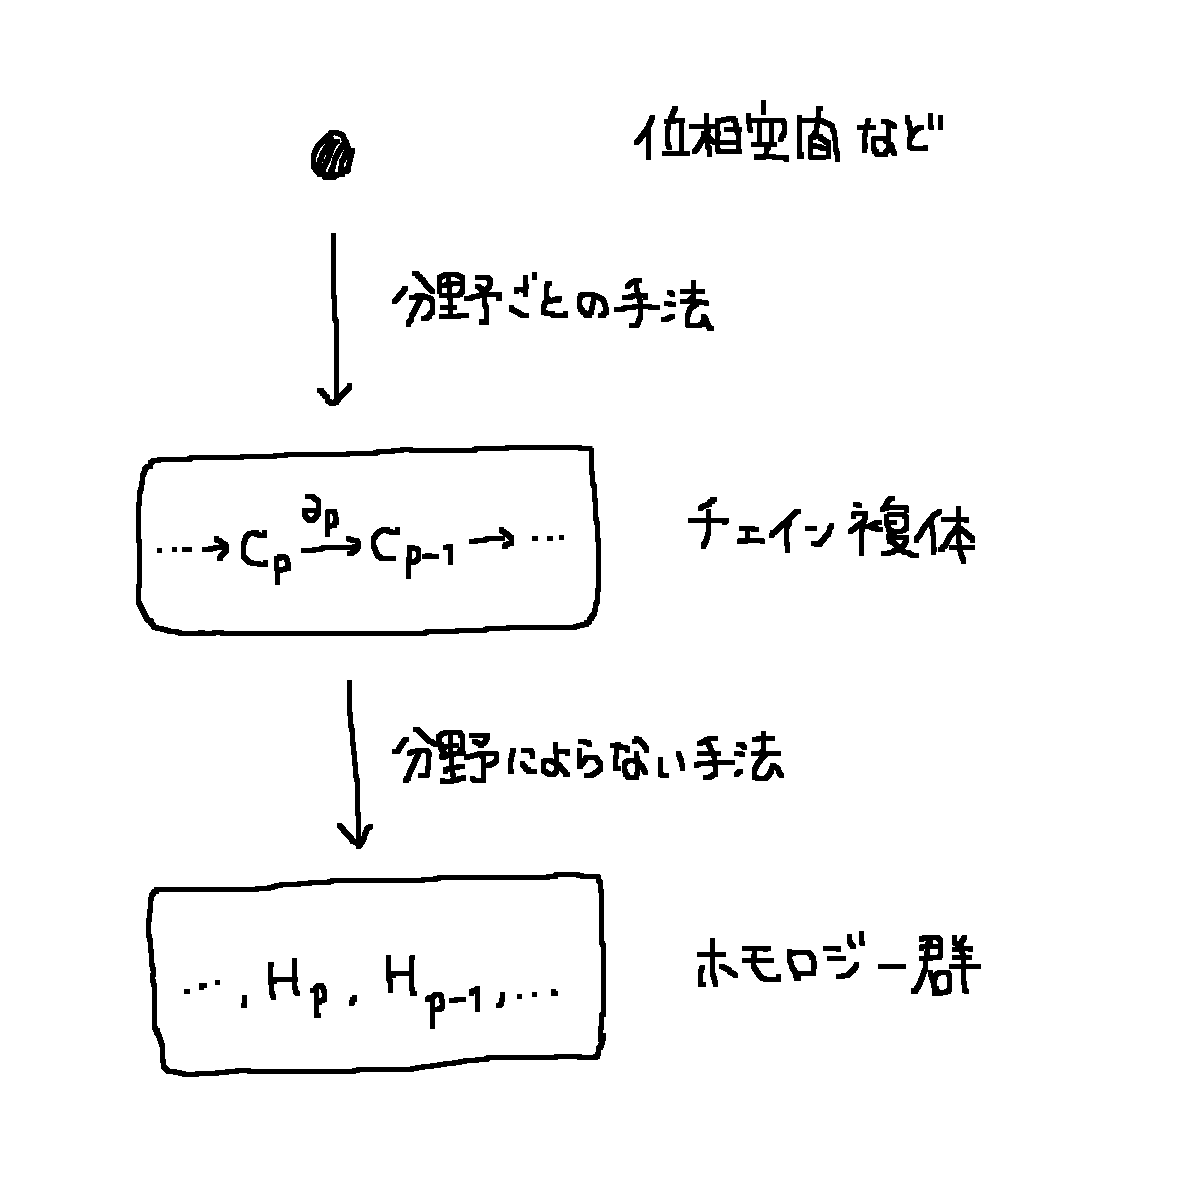
\includegraphics[width=8cm]{\assetspath assets/homology-overview.png}
%    \caption{チェイン複体とホモロジー群}
%    \label[figure]{fig:homology-overview}
%\end{figure}

ホモロジーとは、大まかには位相空間などの対象に
ホモロジー群と呼ばれるアーベル群を対応させる手続きのことである。
ホモロジー群の構成方法は大きく分けて2ステップに分けられる:
\begin{enumerate}
    \item 位相空間などの対象から、チェイン複体と呼ばれる代数的対象を構成し、
    \item チェイン複体からホモロジー群を構成する。
\end{enumerate}
1つ目のステップには分野ごとの手法が用いられるが、
2つ目のステップは純粋に代数的な操作である。
この2つ目のステップを切り出し、位相空間などの具体的対象から切り離して研究する分野はホモロジー代数学と呼ばれる。

ホモロジー群が基本群より優れている点として、
基本群は一般に非アーベルである一方、ホモロジー群はアーベルなので、
非アーベル性に起因する計算上の困難を回避できるという点がある。
また、ホモロジー群では基本群のように基点を選ぶ必要がないため、
位相空間のすべての弧状連結成分の情報を持っているという利点もある。


% ----------------------------------------------------------------------------
%
% ----------------------------------------------------------------------------
\section{アーベル群のチェイン複体}

ここで位相空間から一旦離れて、アーベル群のチェイン複体という代数的対象を定義する。
チェイン複体とは、境界作用素と呼ばれる特別な準同型で繋がれたアーベル群の列のことである。
チェイン複体はCW複体や単体的複体と名前が似ているが、\highlight{全く別物}である。

\subsection{チェイン複体}

チェイン複体を定義する。

\begin{definition}[チェイン複体]
    \idxsym{homologue}{$z \sim z'$}{ホモローグなサイクル}
    アーベル群と準同型の列
    \begin{equation}
        \begin{tikzcd}
            \cdots \ar{r}
            & C_{p+1} \ar{r}{\partial_{p+1}}
            & C_p \ar{r}{\partial_{p}}
            & C_{p-1} \ar{r}
            & \cdots
        \end{tikzcd}
    \end{equation}
    が\term{チェイン複体}[chain complex]{チェイン複体}[ちぇいんふくたい]であるとは、
    すべての$p \in \Z$に対し$\partial_{p} \circ \partial_{p+1} = 0$が成り立つことをいう。
    $\partial_p$らを\term{境界作用素}[boundary operator]{境界作用素}[きょうかいさようそ]といい、
    単に$\partial$と書くこともある。
    チェイン複体を$(C_*, \partial_*)$や$C_*$で表す。
    また、
    \begin{itemize}
        \item $C_p$を\term{第$p$チェイン群}[$p$-th chain group]{チェイン群}[ちぇいんぐん]という。
        \item $C_p$の元を\term{$p$-チェイン}[$p$-chain]{チェイン}[ちぇいん]という。
        \item $\Ker(\partial_{p})$の元を\term{$p$-サイクル}[$p$-cycle]{サイクル}[さいくる]という。
        \item $\Im(\partial_{p+1})$の元を\term{$p$-バウンダリ}[$p$-boundary]{バウンダリ}[ばうんだり]という。
    \end{itemize}
    また、$p$-サイクル$z, z'$の差$z - z'$が$p$-バウンダリであるとき、
    $z \sim z'$と書き、$z, z'$は
    \term{ホモローグ}[homologue]{ホモローグ}であるという。
\end{definition}

\begin{definition}[チェイン写像]\index{チェイン写像}
    $C_*, D_*$をチェイン複体とする。
    準同型の族$F = \{F_p\}_{p \in \Z},\; F_p \colon C_p \to D_p$
    が\emph{チェイン写像 (chain map)}であるとは、図式
    \begin{equation}
        \begin{tikzcd}
            \cdots \ar{r}
            & C_p \ar{r}{\partial_{p}} \ar{d}{F_{p}}
            & C_{p-1} \ar{r} \ar{d}{F_{p-1}}
            & \cdots \\
            \cdots \ar{r}
            & D_p \ar{r}{\partial_{p}}
            & D_{p-1} \ar{r}
            & \cdots
        \end{tikzcd}
    \end{equation}
    が可換であることをいう。
\end{definition}

\begin{definition}[分裂]
    $C = (C_p, \del_p)$をチェイン複体とする。
    $C$が次の条件をみたすとき、
    $C$は\term{分裂}[split]{分裂}[ぶんれつ]するという:
    \begin{itemize}
        \item 準同型の族$\{ s_p \colon C_p \to C_{p + 1} \}$が存在し、
            $\del_{p + 1} \circ s_p \circ \del_{p + 1} = \del_{p + 1}$
            をみたす。
    \end{itemize}
\end{definition}

次の補題は整係数ホモロジー群の計算に役立つ。

\begin{lemma}
    \label[lemma]{lemma:integer-right-exact-lemma}
    アーベル群の完全列
    \begin{equation}
        \begin{tikzcd}
            A \ar{r}{f}
                & \Z \oplus \Z \ar{r}{g}
                & \Z \ar{r}
                & 0
                & (\text{exact})
        \end{tikzcd}
    \end{equation}
    に対し$\Im f \cong \Z$が成り立つ。
\end{lemma}

\begin{proof}
    まず
    \begin{equation}
        \begin{tikzcd}
            0 \ar{r}
                & \Im g \ar[hook]{r}
                & \Z \ar{r}
                & 0
                & (\text{exact})
        \end{tikzcd}
    \end{equation}
    より$\Im g \cong \Z$だから、
    \begin{equation}
        \begin{tikzcd}
            0 \ar{r}
                & \Ker g \ar[hook]{r}
                & \Z \oplus \Z \ar{r}{g}
                & \underbrace{\Im g}_{\cong \Z} \ar{r}
                & 0
                & (\text{exact})
        \end{tikzcd}
    \end{equation}
    が分裂することとあわせて
    $\Z \oplus \Z \cong \Ker g \oplus \Z$である。
    有限生成アーベル群の構造定理より\TODO{とは?}
    $\Z \cong \Ker g \; (= \Im f)$である。
\end{proof}

\subsection{代数的構成}

\begin{definition}[部分複体]
    $C, D$をチェイン複体とする。
    $C$が$D$の\term{部分複体}[subcomplex]{部分複体}[ぶぶんふくたい]であるとは、
    \begin{itemize}
        \item 各$C_p$は$D_p$の部分群
        \item 包含写像の族$\{ C_p \hookrightarrow D_p \}_p$はチェイン写像
    \end{itemize}
    が成り立つことをいう。
\end{definition}

\begin{definition}[商複体]
    \TODO{$\wb{\del}$が誘導される場合しか定義できない?}
\end{definition}

\begin{definition}[和複体]
    \TODO{アーベル群の和とは?}
\end{definition}

\begin{definition}[チェイン複体の柱と錐]
    \idxsym{mapping cylinder}{$Z_f$}{チェイン写像$f$の写像柱}
    \idxsym{mapping cone}{$C_f$}{チェイン写像$f$の写像錐}
    \idxsym{cylinder}{$ZA$}{チェイン複体$A$の柱}
    \idxsym{cone}{$CA$}{チェイン複体$A$の錐}
    $A = (A_p, \del_p), \; B = (B_p, \del_p)$をチェイン複体とし、
    $f \colon A \to B$をチェイン写像とする。
    \begin{itemize}
        \item 次で定義されるチェイン複体$Z_f$を
            $f$の\term{写像柱}[mapping cylinder]{写像柱}[しゃぞうちゅう]という:
            \begin{equation}
                Z_f \coloneqq \left(
                    A_p \oplus A_{p - 1} \oplus B_p,
                    \begin{bmatrix}
                        \del & \id & 0 \\
                        0 & -\del & 0 \\
                        0 & -f & \del
                    \end{bmatrix}
                \right)
            \end{equation}
            ただし、行列の意味は
            \begin{equation}
                \del_p(a, a', b) = (
                    \del_p a + a', \; - \del_{p - 1} a', \; \del_p b - f(a')
                )
            \end{equation}
            ということである。
        \item 次で定義されるチェイン複体$C_f$を
            $f$の\term{写像錐}[mapping cone]{写像錐}[しゃぞうすい]という:
            \begin{equation}
                C_f \coloneqq \left(
                    A_{p - 1} \oplus B_p,
                    \begin{bmatrix}
                        -\del & 0 \\
                        -f & \del
                    \end{bmatrix}
                \right)
            \end{equation}
        \item 恒等写像$\id_A$の写像柱$Z_\id$を$ZA$と書き、
            $A$の\term{柱}[cylinder]{柱}[ちゅう]という。
        \item 恒等写像$\id_A$の写像錐$C_\id$を$CA$と書き、
            $A$の\term{錐}[cone]{錐}[すい]という。
    \end{itemize}
\end{definition}

\subsection{チェインホモトピー}

\begin{definition}[チェインホモトピー]
    $C, D$をチェイン複体とし、
    $f, g \colon C \to D$をチェイン写像とする。
    \begin{itemize}
        \item $f$と$g$が
            \term{チェインホモトピック}[chain homotopic]{チェインホモトピック}
            であるとは、ある\highlight{写像}の族
            $\{ s_n \colon C_n \to D_{n + 1} \}_n$が存在して
            \begin{equation}
                f - g = s \circ \del + \del \circ s
            \end{equation}
            が成り立つことをいう\TODO{準同型ではないか?}。
            この写像族$\{ s_n \}$を$f$から$g$への
            \term{チェインホモトピー}[chain homotopy]{チェインホモトピー}
            という。
            \begin{equation}
                \begin{tikzcd}[column sep=large, row sep=large]
                    & C_n
                        \ar{r}{\del}
                        \ar{d}{f - g}
                        \ar{ld}[swap]{s}
                        & C_{n - 1} \ar{ld}{s} \\
                    D_{n + 1} \ar{r}[swap]{\del}
                        & D_n
                \end{tikzcd}
            \end{equation}
        \item $f$が
            \term{チェインホモトピー同値写像}[chain homotopy equivalence]
            {チェインホモトピー同値写像}[ちぇいんほもとぴーどうちしゃぞう]
            であるとは、
            あるチェイン写像$h \colon D \to C$が存在して、
            $h \circ f$が$\id_C$と、$f \circ h$が$\id_D$と
            それぞれチェインホモトピックであることをいう。
    \end{itemize}
\end{definition}

\subsection{ホモロジー群}

チェイン複体に対しホモロジー群を定義する。
ホモロジー群は、チェイン複体が完全からどれほどずれているかを測る指標である。

\begin{definition}[ホモロジー群]
    $C_*$をチェイン複体とする。各$p \in \Z$に対し、
    \begin{equation}
        H_p(C_*) \coloneqq \Ker(\partial_{p}) / \Im(\partial_{p+1})
    \end{equation}
    を$C_*$の\term{第$p$ホモロジー群}[$p$-th homology group]{ホモロジー群!チェイン複体の---}という。
\end{definition}

\begin{definition}[チェイン写像から誘導される群準同型]
    \TODO{チェイン写像はホモロジー群の間の準同型を誘導する}
\end{definition}

\begin{definition}[擬同型]
    $f \colon C \to D$をチェイン写像とする。
    $f$の誘導する群準同型$f_* \colon H_p(C) \to H_p(D)$が
    すべての$p \in \Z$に対し同型であるとき、
    $f$は\term{擬同型}[quisi-isomorphism; quism]{擬同型}[ぎどうけい]であるという。
\end{definition}

\begin{theorem}[チェインホモトピーと誘導される群準同型]
    \TODO{}
\end{theorem}

\begin{proof}
    \TODO{}
\end{proof}

次の定理は後々
\cref{subsection:betti-number-and-euler-characteristic}
で導入する Betti 数や Euler 標数と深く関係している。

\begin{theorem}[Euler-Poincar\'e の原理]
    \label[theorem]{thm:euler-poincare-theorem}
    $C = (C_p, \del_p)$を有限生成アーベル群からなる有界なチェイン複体とする。
    このとき
    \begin{equation}
        \sum_{p} (-1)^p \rk C_p
            = \sum_{p} (-1)^p \rk H_p(C)
    \end{equation}
    が成り立つ。
\end{theorem}

\begin{proof}
    ホモロジー代数学の基本的な結果により、
    有限生成アーベル群の短完全列
    \begin{equation}
        \begin{tikzcd}
            0
                \ar{r}
                & X
                    \ar{r}
                & Y
                    \ar{r}
                & Z
                    \ar{r}
                & 0
        \end{tikzcd}
    \end{equation}
    に対し
    $\rk Y = \rk X + \rk Z$が成り立つ。
    いまチェイン複体$C$に対し
    \begin{gather}
        \begin{tikzcd}[ampersand replacement=\&]
            0
                \ar{r}
                \& B_p(C)
                    \ar{r}
                \& Z_p(C)
                    \ar{r}
                \& H_p(C)
                    \ar{r}
                \& 0
                \& (\text{exact})
        \end{tikzcd} \\
        \begin{tikzcd}[ampersand replacement=\&]
            0
                \ar{r}
                \& Z_p(C)
                    \ar{r}
                \& C_p
                    \ar{r}
                \& B_{p - 1}(C)
                    \ar{r}
                \& 0
                \& (\text{exact})
        \end{tikzcd}
    \end{gather}
    が成り立つから
    \begin{alignat}{1}
        \sum_p (-1)^p \rk C_p
            &= \sum_p (-1)^p \rk Z_p(C)
                + \sum_p (-1)^p \rk B_{p - 1}(C) \\
            &= \sum_p (-1)^p \rk Z_p(C)
                - \sum_p (-1)^p \rk B_p(C) \\
            &= \sum_p (-1)^p \rk H_p(C)
    \end{alignat}
    を得る。
\end{proof}




% ----------------------------------------------------------------------------
%
% ----------------------------------------------------------------------------
\section{アファインホモロジー}

位相空間に戻り、アファインチェイン複体を定義する。
\TODO{アファインチェイン複体は特異ホモロジーの議論に使われる以上の役割はあるのだろうか?}

\begin{definition}[アファイン単体]
    \idxsym{standard simplex}{$\Delta^k$}{標準$k$-単体}
    \idxsym{convex polyhedron}{$|[v_0 \dots v_k]|$}{凸多面体}
    \idxsym{affine simplex}{$[v_0 \dots v_k]$}{アファイン$k$-単体}
    \idxsym{affine simplices}{$S_k^\aff(X)$}{$X$内のアファイン$k$-単体全体}
    \idxsym{free abelian group of $k$-chains}{$C_k^\aff(X)$}{$X$内のアファイン$k$-チェイン全体}
    $A \subset \R^n$を\highlight{凸部分集合}、
    $k \in \Z_{\ge 0}$、
    $v_0, \dots, v_k \in A$とする。
    \begin{itemize}
        \item $\R^{k + 1}$の標準基底$e_0, \dots, e_k$の凸包を
            $\Delta^{k}$と書き、
            \term{標準$k$-単体}[standard $k$-simplex]{標準単体}[ひょうじゅんたんたい]
            という。
        \item アファイン写像
            \begin{equation}
                [v_0 \dots v_k] \coloneqq \Delta^k \to A,
                \quad
                e_i \mapsto v_i \quad (i = 0, \dots, k)
            \end{equation}
            を$A$内の
            \term{アファイン$k$-単体}[affine $k$-simplex]{アファイン単体}[あふぁいんたんたい]
            という。
        \item 集合
            \begin{equation}
                |[v_0 \dots v_k]| \coloneqq \left\{
                    \sum_{i=0}^k t_i v_i
                    \; \bigg| \;
                    t_i \ge 0,\; \sum_{i=0}^k t_i = 1
                \right\}
            \end{equation}
            を$v_0, \dots, v_k$を頂点とする
            \term{凸多面体}[convex polyhedron]{凸多面体}[とつためんたい]という。
        \item $A$内のアファイン$k$-単体の全体を
            \begin{alignat}{1}
                S_k^\aff(A)
                    &\coloneqq \{
                        \text{$A$内のアファイン$k$-単体}
                    \} \\
                    &= \{
                        \sigma \colon \Delta^k \to A
                        \mid
                        \sigma \text{ はアファイン写像}
                    \}
            \end{alignat}
            で表す。
        \item $S_p^\aff(A)$により生成される自由アーベル群を
            $C_p^\aff(A)$と書き、
            $C_p^\aff(A)$の元を$A$内の\term{アファイン$p$-チェイン}[affine $p$-chain]
            {アファインチェイン}[あふぁいんちぇいん]
            という。
        \item 各$i \in \{0, \dots, k\}$に対し、
            アファイン写像$F_i \colon \Delta^{k - 1} \to \Delta^{k}$を
            \begin{equation}
                F_i(e_j) \coloneqq \begin{cases}
                    e_j & (j < i) \\
                    e_{j + 1} & (j \ge i)
                \end{cases}
            \end{equation}
            で定め、これを
            \term{面写像}[face map]{面写像}[めんしゃぞう]
            という。
            $F_i$による引き戻しで
            写像$F_i^* \colon C_k^\aff(A) \to C_{k - 1}^\aff(A)$が
            \begin{equation}
                F_i^* [v_0 \dots v_k]
                    = [
                        v_0
                        \dots
                        \what{v}_i
                        \dots
                        v_k
                    ]
            \end{equation}
            と定まる。
            \begin{equation}
                \begin{tikzcd}[column sep=large]
                    \Delta^k
                        \ar{r}{[v_0 \dots v_k]}
                        & A \\
                    \Delta^{k - 1}
                        \ar{u}{F_i}
                        \ar{ru}[swap]{F_i^* [v_0 \dots v_k]}
                \end{tikzcd}
            \end{equation}
        \item 写像$\del_k \colon C_k^\aff(A) \to C_{k - 1}^\aff(A)$を
            次のように定める:
            各$[v_0 \dots v_k] \in S_k^\aff(A)$に対し
            \begin{equation}
                \del_k [v_0 \dots v_k]
                    \coloneqq \sum_{i = 0}^k (-1)^i F_i^* [v_0 \dots v_k]
            \end{equation}
            と定め、$C_k^\aff(A)$上まで$\Z$-線型に拡張する。
            $\del_k$を
            \term{境界作用素}[boundary operator]{境界作用素}[きょうかいさようそ]
            という。
    \end{itemize}
\end{definition}

\begin{proposition}
    任意の$k \in \Z$に対し
    $\del_k \circ \del_{k + 1} = 0$
    が成り立つ。
\end{proposition}

\begin{remark}
    この命題により
    \begin{equation}
        \begin{tikzcd}
            \cdots \ar{r}
            & C^\aff_{k + 1}(A) \ar{r}{\partial_{k + 1}}
            & C^\aff_k(A) \ar{r}{\partial_{k}}
            & C^\aff_{k - 1}(A) \ar{r}
            & \cdots
        \end{tikzcd}
    \end{equation}
    はアーベル群のチェイン複体となる。
\end{remark}

\begin{proof}
    \TODO{}
\end{proof}

\begin{example}[{$[ab]$と$-[ba]$はホモローグ}]
    $A \subset \R^n$を凸部分集合とし、$a, b \in A$とする。
    \begin{equation}
        [ab] \sim -[ba]
        \quad \text{すなわち} \quad
        [ab] + [ba] \in \Im \del_2
    \end{equation}
    が成り立つことを示す。
    そこで$2$-単体$[aba], [aaa]$をそれぞれ$\del_2$で写すと
    \begin{alignat}{1}
        \del_2 [aba] &= [ba] - [aa] + [ab] \\
        \del_2 [aaa] &= [aa] - [aa] + [aa] = [aa]
    \end{alignat}
    となるから
    \begin{alignat}{1}
        [ab] + [ba]
            &= \del_2 [aba] + \del_2 [aaa] \\
            &= \del_2 ([aba] + [aaa]) \\
            &\in \Im \del_2
    \end{alignat}
    より$[ab] \sim -[ba]$が従う。
\end{example}

\subsection{プリズム構成}

プリズム構成は、
$k$-チェインから$(k + 1)$-チェインを構成する方法であり、
特異ホモロジーのホモトピー不変性の証明に用いられる。

\begin{definition}[プリズム構成]
    $A \subset \R^n$を凸部分集合とする。
    写像$i_k \; (k = 0, 1)$を
    \begin{equation}
        i_k \colon A \to A \times I,
        \quad
        x \mapsto (x, k)
    \end{equation}
    と定める。
    各$\alpha = [v_0 \dots v_p] \in S_p^\aff(A)$に対し
    $v_{ij} \coloneqq (v_i, j) \in A \times I$と書くことにする。
    このとき
    \begin{alignat}{1}
        i_{0*} \alpha &= [v_{00} \dots v_{p0}] \\
        i_{1*} \alpha &= [v_{01} \dots v_{p1}]
    \end{alignat}
    である。
    ここで$\alpha \in S_p^\aff(A)$の
    \term{プリズム}[prism]{プリズム}[ぷりずむ]
    $\Pi_p \alpha$を
    \begin{equation}
        \Pi_p \alpha \coloneqq
            \sum_{i = 0}^p (-1)^i [
                v_{00}
                \dots
                \underbrace{v_{i0} v_{i1}}_{\mathclap{i \text{ 番目で上にあがる}}}
                \dots
                v_{p1}
            ]
            \in C_{p + 1}^\aff(A \times I)
    \end{equation}
    と定め、
    $C_p^\aff(A)$上まで$\Z$-線型に拡張して
    群準同型
    $\Pi_p \colon C_p^\aff(A) \to C_{p + 1}^\aff(A \times I)$を定義する。
\end{definition}

\begin{proposition}[プリズム構成の公式]
    \TODO{}
\end{proposition}

\begin{remark}
    この命題より、
    $\Pi_p \colon C_p^\aff(A) \to C_{p + 1}^\aff(A \times I)$
    はチェイン写像
    $i_{0*}, i_{1*} \colon C_p^\aff(A) \to C_p^\aff(A \times I)$
    をつなぐチェインホモトピーであることがわかる。
\end{remark}

\begin{proof}
    \TODO{}
\end{proof}

\subsection{重心細分}

\TODO{切除定理のところでしか使わないので、そこで述べるべき?}

% ----------------------------------------------------------------------------
%
% ----------------------------------------------------------------------------
\section{特異ホモロジー}

一般の空間に対し特異ホモロジー群を定義する。
特異ホモロジー群は直接計算するには適さないが、
理論的には重要な役割を果たす。

\subsection{定義と基本性質}

\begin{definition}[特異単体]
    \idxsym{singular simplices}{$S_p^\sing(X)$}{$X$内の特異$p$-単体全体}
    \idxsym{free abelian group of $p$-chains}{$C_p^\sing(X)$}
        {$X$内の特異$p$-チェイン全体}
    $X$を位相空間、$p \in \Z$とする。
    \begin{itemize}
        \item 連続写像$\Delta^p \to X$を
            $X$内の
            \term{特異$p$-単体}[singular $p$-simplex]{特異単体}[とくいたんたい]
            という。
        \item $X$内の特異$p$-単体の全体を
            \begin{alignat}{1}
                S_p^\sing(X)
                    &\coloneqq \{
                        \text{$X$内の特異$p$-単体}
                    \} \\
                    &= \{
                        \sigma \colon \Delta^p \to X
                        \mid
                        \sigma \text{ は連続写像}
                    \}
            \end{alignat}
            で表す。
        \item $S_p^\sing(X)$により生成される自由アーベル群を
            $C_p^\sing(X)$と書き、
            $C_p^\sing(X)$の元を$X$内の\term{特異$p$-チェイン}[singular $p$-chain]
            {特異チェイン}[とくいちぇいん]
            という。
        \item \term{境界作用素}[boundary operator]{境界作用素}[きょうかいさようそ]
            と呼ばれる
            写像$\del_p \colon C_p^\sing(X) \to C_{p - 1}^\sing(X)$を
            次のように定める:
            各$\sigma \in S_p^\sing(X)$に対し
            \begin{equation}
                \del_p \sigma
                    \coloneqq
                    \sum_{i = 0}^p (-1)^i F_i^* \sigma
            \end{equation}
            と定め、$C_p^\sing(X)$上まで$\Z$-線型に拡張する。
    \end{itemize}
\end{definition}

\begin{proposition}
    任意の$p \in \Z$に対し
    $\del_p \circ \del_{p + 1} = 0$
    が成り立つ。
\end{proposition}

\begin{remark}
    この命題により
    \begin{equation}
        \begin{tikzcd}
            \cdots \ar{r}
            & C^\sing_{p + 1}(X) \ar{r}{\partial_{p + 1}}
            & C^\sing_p(X) \ar{r}{\partial_{p}}
            & C^\sing_{p - 1}(X) \ar{r}
            & \cdots
        \end{tikzcd}
    \end{equation}
    はアーベル群のチェイン複体となる。
\end{remark}

\begin{proof}
    \TODO{}
\end{proof}

\begin{definition}[連続写像から誘導されるチェイン写像]
    \TODO{$f_\sharp$}
\end{definition}

\begin{definition}[特異ホモロジー群]
    \TODO{}
\end{definition}

\begin{definition}[$\Z$-加群を係数にもつ特異ホモロジー群]
    $X$を位相空間、$p \in \Z$、
    $A$を$\Z$-加群とする。
    テンソル積関手$C_p(X) \otimes_\Z \Box$により
    \begin{alignat}{1}
        C_p(X) &\mapsto C_p(X; A) \coloneqq C_p(X) \otimes_\Z A \\
        \del_p &\mapsto \del^A_p \coloneqq \del_p \otimes \id_A
    \end{alignat}
    と写したチェイン複体$C(X; A) \coloneqq (C_p(X; A), \del^A_p)$から得られる
    ホモロジー群$H_p(X; A) \coloneqq H_p(C(X; A))$を
    \term{$A$-係数特異ホモロジー群}{$\Z$-加群を係数にもつ特異ホモロジー群}
    [Zかぐんをけいすうにもつとくいほもろじーぐん]
    という。
\end{definition}

\begin{remark}
    上の定義で得られたホモロジー群$H_p(X; A)$は、
    一般には$H_p(X) \otimes_\Z A$とは異なることに注意。
    定義のようにチェイン群の段階でテンソル積をとる必要がある。

    \TODO{普遍係数定理?}
\end{remark}

\begin{definition}[特異チェインのプリズム]
    $X$を位相空間、$p \in \Z$とする。
    $\sigma \in S_p^\sing(X)$に対し、
    $\sigma$の
    \term{プリズム}[prism]{プリズム}[ぷりずむ]
    $\Pi_p \sigma$を次のように定める:
    $[v_0 \dots v_p] \coloneqq \id_{\Delta^p} \in S_p^\aff(\Delta^p)$とおき、
    \begin{equation}
        \Pi_p \sigma \coloneqq
            \sum_{i = 0}^p (-1)^i
            (\sigma \times \id_I) \circ
            [
                v_{00}
                \dots
                \underbrace{v_{i0} v_{i1}}_{\mathclap{i \text{ 番目で上にあがる}}}
                \dots
                v_{p1}
            ]
            \in C_{p + 1}^\sing(X \times I)
    \end{equation}
    と定め、
    $C_p^\sing(X)$上まで$\Z$-線型に拡張して
    群準同型
    $\Pi_p \colon C_p^\sing(X) \to C_{p + 1}^\sing(X \times I)$を定義する。
    \TODO{もっとアファインチェインのプリズムの定義をそのまま利用する定義にできないか?}
\end{definition}

\begin{example}[$0$次ホモロジー]
    \TODO{}
    $X$が弧状連結なら
    \begin{equation}
        H_0(X) \cong \Z
    \end{equation}
    である。
\end{example}

\subsection{ホモトピー不変性}

\begin{theorem}[特異ホモロジー群のホモトピー不変性]
    $X, Y$を位相空間とする。
    $X, Y$がホモトピー同値ならば、
    $H_p(X), H_p(Y)$は同型である ($p \in \Z$)。
    とくに特異ホモロジー群は位相不変量である。
\end{theorem}

\begin{proof}
    \TODO{}
\end{proof}

プリズム分解を用いて次が示される\footnote{
    [河澄] では acyclic model theorem を用いて証明している。
}。

\begin{theorem}[誘導準同型のホモトピー不変性]
    $f, g \colon X \to Y$を互いにホモトピックな連続写像とする。
    このとき、各$p \in \Z$に対し
    $f_*, g_* \colon H_p(X) \to H_p(Y)$は互いに一致する。
\end{theorem}

\begin{proof}
    $f \simeq g$より
    ある連続写像$H \colon X \times I \to Y$が存在して図式
    \begin{equation}
        \begin{tikzcd}
            X \ar{d}[swap]{x \mapsto H(x, 1)} \ar{rd}{g} \\
            X \times I \ar{r}{H}
                & Y \\
            X \ar{u}{x \mapsto H(x, 0)} \ar{ru}[swap]{f}
        \end{tikzcd}
    \end{equation}
    が可換となる。
    \TODO{}
\end{proof}

\cref{def:retraction}で空間のレトラクトを定義した。
レトラクトは一般にホモトピー同値ではないから
包含写像から誘導される準同型は同型とは限らないが、
もう少し弱い主張なら成り立つ。

\begin{proposition}[レトラクトの包含準同型は単射]
    \TODO{}
\end{proposition}

\begin{proof}
    \TODO{}
\end{proof}

レトラクトの概念を用いて次が示せる。

\begin{theorem}[Brouwer の不動点定理]
    \termhidden{Brouwer の不動点定理}[Brouwer のふどうてんていり]
    連続写像$f \colon D^n \to D^n$は
    固定点を持つ。
\end{theorem}

\begin{proof}
    \cref{problem:geometry2-ex-42}を参照。
\end{proof}

\subsection{1点空間のホモロジー}

\begin{example}[1点空間のホモロジー]
    \label[example]{example:homology-of-a-point}
    \TODO{}
    $\mathrm{Pt}$を1点空間として
    \begin{equation}
        H_p(\mathrm{Pt}) = \begin{cases}
            \Z & p = 0 \\
            0 & p \ge 1
        \end{cases}
    \end{equation}
    である。
    したがって$X = \{ x_1, \dots, x_k \}$のとき
    \begin{equation}
        H_p(X) = \begin{cases}
            \Z^k & p = 0 \\
            0 & p \ge 1
        \end{cases}
    \end{equation}
    となる。
\end{example}

\subsection{加法性}

特異ホモロジーは次の意味での加法性をみたす。

\begin{proposition}[特異ホモロジーの加法性]
    \label[proposition]{prop:additivity-of-singular-homology}
    $X$を位相空間、
    $X = \coprod_{\lambda \in \Lambda} X_\lambda$を弧状連結成分への分解とする。
    このとき各$\sigma \colon \Delta^p \to X$の像は
    ただひとつの$\lambda \in \Lambda$に対し
    $\sigma(\Delta^p) \subset X_\lambda$をみたす。
    したがって
    \begin{equation}
        S_p(X) = \coprod_{\lambda \in \Lambda} S_p(X_\lambda),
        \quad
        C_p(X) = \bigoplus_{\lambda \in \Lambda} C_p(X_\lambda),
        \quad
        H_p(X) = \bigoplus_{\lambda \in \Lambda} H_p(X_\lambda)
    \end{equation}
    が成り立つ。
\end{proposition}

\begin{proof}
    \TODO{}
\end{proof}

\subsection{Mayer-Vietoris の定理}

このあと導入する Mayer-Vietoris の定理を用いると、
位相空間の開被覆を用いてホモロジーを計算することができる。
まずジグザグ補題とよばれる定理を示す。
これはチェイン複体の短完全列からホモロジーの長完全列が導かれることを示すものである。

\begin{lemma}[ジグザグ補題]
    \termhidden{ジグザグ補題}[じぐざぐほだい]
    $A, B, C$をアーベル群のチェイン複体とし、
    \begin{equation}
        \begin{tikzcd}
            0 \ar{r}
                & A \ar{r}
                & B \ar{r}
                & C \ar{r}
                & 0
                & (\text{exact})
        \end{tikzcd}
    \end{equation}
    は完全系列であるとする。
    このとき次が成り立つ:
    \begin{enumerate}
        \item 各$p \in \Z$に対し系列
            \begin{equation}
                \begin{tikzcd}
                    H_p(A) \ar{r}
                        & H_p(B) \ar{r}
                        & H_p(C)
                \end{tikzcd}
            \end{equation}
            は完全である。
        \item 各$p \in \Z$に対し
            \term{連結準同型}[connecting homomorphism]
            {連結準同型}[れんけつじゅんどうけい]
            と呼ばれる群準同型
            $\del_* \colon H_p(C) \to H_{p-1}(A)$
            を構成できる。
        \item 各$p \in \Z$に対し系列
            \begin{equation}
                \begin{tikzcd}
                    H_p(A) \ar{r}
                        & H_p(C) \ar{r}{\del_*}
                        & H_{p-1}(A) \ar{r}
                        & H_{p-1}(B)
                \end{tikzcd}
            \end{equation}
            は完全である。
    \end{enumerate}
\end{lemma}

\begin{remark}
    上の補題の状況は補助的な図で
    \begin{equation}
        \begin{tikzcd}
            H(A) \ar{rr}
                && H(B) \ar{ld} \\
            & H(C) \ar{lu}{\del_*}
        \end{tikzcd}
    \end{equation}
    と表される。
    したがって上の補題は
    \term{Exact Triangle}{Exact Triangle}
    とも呼ばれる。
\end{remark}

\begin{proof}
    \TODO{}
\end{proof}

\begin{lemma}
    $X$を位相空間、
    $U, V \subset X, \; X = \Int U \cup \Int V$
    とする。
    チェイン複体の包含写像
    $i \colon C(U) + C(V) \to C(X)$
    は、各$p \in \Z$に対し群の同型
    $H_p(C(U) + C(V)) \to H_p(C(X)) = H_p(X)$
    を誘導する。
\end{lemma}

\begin{proof}
    $p \in \Z$とし、
    $i_* \colon H_p(C(U) + C(V)) \to H_p(C(X))$
    が全単射であることを示す。
    まず$i_*$は全射である。
    \begin{innerproof}
        $[c] \in H_p(X), \; c \in Z_p(X)$とする。
        \TODO{}
    \end{innerproof}
\end{proof}

\begin{theorem}[Mayer-Vietoris]
    $X$を位相空間、
    $X_0, X_1 \subset X, \; X = \Int X_0 \cup \Int X_1$
    とする。
    包含写像を次のようにおく:
    \begin{equation}
        \begin{tikzcd}
            & X_0 \ar[end anchor=north west]{dr}{j_0} \\
            X_0 \cap X_1
                \ar[start anchor=north east]{ur}{i_0}
                \ar[start anchor=south east]{dr}[swap]{i_1}
                & & X_0 \cup X_1 = X \\
            & X_1 \ar[end anchor=south west]{ur}[swap]{j_1}
        \end{tikzcd}
    \end{equation}
    このとき次の系列は完全である:
    \begin{equation}
        \begin{tikzcd}[column sep=large, row sep=large]
            && \cdots
                \ar{r} \ar[phantom]{d}[name=X1, anchor=center]{}
                & H_{p+1}(X)
                    \ar[rounded corners,
                        to path={
                            -- ([xshift=2ex]\tikztostart.east)
                            |- (X1.center) \tikztonodes
                            -| ([xshift=-2ex]\tikztotarget.west)
                            -- (\tikztotarget)
                        }]{dll}[at end, swap]{\partial_*} \\
            & H_p(X_0 \cap X_1)
                \ar{r}{(i_{0*}, -i_{1*})}
                & H_p(X_0) \oplus H_p(X_1)
                    \ar{r}{j_{0*} + j_{1*}}
                    \ar[phantom]{d}[name=X2, anchor=center]{}
                & H_p(X)
                    \ar[rounded corners,
                        to path={
                            -- ([xshift=2ex]\tikztostart.east)
                            |- (X2.center) \tikztonodes
                            -| ([xshift=-2ex]\tikztotarget.west)
                            -- (\tikztotarget)
                        }]{dll}[at end, swap]{\partial_*} \\
            & H_{p-1}(X_0 \cap X_1)
                \ar{r}
                & \cdots
        \end{tikzcd}
    \end{equation}
    この系列を$(X, X_0, X_1)$の
    \term{Mayer-Vietoris 完全系列}[Mayer-Vietoris sequence]
    {Mayer-Vietoris 完全系列}[Mayer-Vietorisかんぜんけいれつ]
    という。
\end{theorem}

\begin{proof}
    \TODO{}
\end{proof}

Mayer-Vietoris の定理を用いた計算の例として
$S^n$の特異ホモロジー群を求めてみる。
この結果は単にホモロジーの計算例のひとつというばかりでなく、
後で導入する写像度や胞体的ホモロジーなどの発展的概念の基礎となる。

\begin{theorem}[$S^n$の特異ホモロジー群]
    \label[theorem]{thm:sphere-singular-homology}
    球面$S^n$の特異ホモロジー群$H_p(S^n)$は次の表のとおりである:
    \begin{center}
        \begin{tabular}{|c|c|c|c|c|}
            \hline
            \diagbox{$p$}{$n$} & 0 & 1 & 2 & $\cdots$ \\
            \hline
            0 & $\Z \oplus \Z$ & $\Z$ & $\Z$ & $\cdots$ \\
            \hline
            1 & $0$ & $\Z$ & $0$ & $\cdots$ \\
            \hline
            2 & $0$ & $0$ & $\Z$ & $\cdots$ \\
            \hline
            $\vdots$ & $\vdots$ & $\vdots$ & $\vdots$ & $\ddots$ \\
            \hline
        \end{tabular}
    \end{center}
\end{theorem}

\begin{proof}
    $S^n$の北極を$N$、南極を$S$とおき、
    \begin{equation}
        U_+ \coloneqq S^n \setminus \{ S \} \opensubset S^n,
        \quad
        U_- \coloneqq S^n \setminus \{ N \} \opensubset S^n
    \end{equation}
    とおく。
    $\mathrm{Pt}$を1点空間として
    \begin{equation}
        U_+ \cap U_- \simeqhe S^{n - 1},
        \quad
        U_+ \simeqhe N = \mathrm{Pt},
        \quad
        U_- \simeqhe S = \mathrm{Pt}
    \end{equation}
    が成り立つから、$(S^n, U_+, U_-)$の Mayer-Vietoris 完全系列は
    \begin{equation}
        \begin{tikzcd}[column sep=large, row sep=large]
            && \cdots \ar{r} \ar[phantom]{d}[name=X1, anchor=center]{}
                & H_{p+1}(S^n) \ar[rounded corners,
                        to path={
                            -- ([xshift=2ex]\tikztostart.east)
                            |- (X1.center) \tikztonodes
                            -| ([xshift=-2ex]\tikztotarget.west)
                            -- (\tikztotarget)
                        }]{dll} \\
            & H_p(S^{n - 1}) \ar{r}
                & H_p(\mathrm{Pt}) \oplus H_p(\mathrm{Pt})
                    \ar{r} \ar[phantom]{d}[name=X2, anchor=center]{}
                & H_p(S^n) \ar[rounded corners,
                        to path={
                            -- ([xshift=2ex]\tikztostart.east)
                            |- (X2.center) \tikztonodes
                            -| ([xshift=-2ex]\tikztotarget.west)
                            -- (\tikztotarget)
                        }]{dll} \\
            & H_{p-1}(S^{n - 1}) \ar{r}
                & \cdots
        \end{tikzcd}
    \end{equation}
    となる。
    \cref{example:homology-of-a-point}より
    \begin{equation}
        H_p(\mathrm{Pt}) \cong \begin{cases}
            0 & (p \ge 1) \\
            \Z & (p = 0)
        \end{cases}
    \end{equation}
    であったから、次を得る:
    \begin{enumerate}
        \item $p \ge 2$のとき
            \begin{equation}
                \begin{tikzcd}
                    0 \ar{r}
                        & H_p(S^n) \ar{r}
                        & H_p(S^{n - 1}) \ar{r}
                        & 0
                        & (\text{exact})
                \end{tikzcd}
            \end{equation}
            が完全であることより
            $H_p(S^n) \cong H_{p - 1}(S^{n - 1})$となる。
        \item $p = 1$のとき
            \begin{equation}
                \begin{tikzcd}
                    0 \ar{r}
                        & H_1(S^n) \ar{r}
                        & H_0(S^{n - 1}) \ar{r}
                        & \Z \oplus \Z \ar{r}
                        & H_0(S^n) \ar{r}
                        & 0
                        & (\text{exact})
                \end{tikzcd}
            \end{equation}
            は完全である。
            \begin{enumerate}[label=(\arabic{enumi}-\alph*)]
                \item $n = 1$のとき、
                    $S^0 = \{ \pm 1 \}$であることと
                    $S^1$が弧状連結であることより
                    \begin{equation}
                        \begin{tikzcd}
                            0 \ar{r}
                                & H_1(S^1) \ar{r}
                                & \underbrace{H_0(S^0)}_{\Z \oplus \Z} \ar{r}
                                & \Z \oplus \Z \ar{r}
                                & \underbrace{H_0(S^1)}_{\Z} \ar{r}
                                & 0
                                & (\text{exact})
                        \end{tikzcd}
                    \end{equation}
                    を得る。
                    したがって$H_1(S^1) \cong \Z$である (このあと示す)。
                \item $n \ge 2$のとき、
                    $S^{n - 1}, S^n$が弧状連結であることより
                    \begin{equation}
                        \begin{tikzcd}
                            0 \ar{r}
                                & H_1(S^n) \ar{r}
                                & \underbrace{H_0(S^{n - 1})}_{\Z} \ar{r}
                                & \Z \oplus \Z \ar{r}
                                & \underbrace{H_0(S^n)}_{\Z} \ar{r}
                                & 0
                                & (\text{exact})
                        \end{tikzcd}
                    \end{equation}
                    を得る。
                    したがって$H_1(S^n) \cong 0$である (このあと示す)。
            \end{enumerate}
    \end{enumerate}
    (2-a), (2-b) の結論を証明する。
    (2-a) の完全系列の各射に名前をつけて
    \begin{equation}
        \begin{tikzcd}
            0 \ar{r}{f_1}
                & H_1(S^1) \ar{r}{f_2}
                & \Z \oplus \Z \ar{r}{f_3}
                & \Z \oplus \Z \ar{r}{f_4}
                & \Z \ar{r}{f_5}
                & 0
                & (\text{exact})
        \end{tikzcd}
    \end{equation}
    とおく。
    有限ランク自由$\Z$-加群の Rank-Nullity Theorem を
    右側から順次適用して
    \begin{alignat}{1}
        \rk\Im f_4 &= \rk\Ker f_5 = \rk\Z - \rk\Im f_5 = 1 - 0 = 1 \\
        \rk\Im f_3 &= \rk\Ker f_4 = \rk(\Z \oplus \Z) - \rk\Im f_4 = 2 - 1 = 1 \\
        \rk\Im f_2 &= \rk\Ker f_3 = \rk(\Z \oplus \Z) - \rk\Im f_3 = 2 - 1 = 1
    \end{alignat}
    を得る。
    \TODO{本当か?}
    したがって$\Im f_2 \cong \Z$だから、完全系列
    \begin{equation}
        \begin{tikzcd}
            0 \ar{r}
                & H_1(S^1) \ar{r}
                & \Z \ar{r}
                & 0
                & (\text{exact})
        \end{tikzcd}
    \end{equation}
    を得る。よって (2-a) の結論$H_1(S^1) \cong \Z$がたしかに成り立つ。
    同様にして (2-b) の結論$H_1(S^n) \cong 0$も成り立つ。
    以上をまとめて定理の表を得る。
\end{proof}

\begin{corollary}
    $m, n \in \Z_{\ge 1}$が
    $m \neq n$ならば
    $\R^m \not\approx \R^n$である。
\end{corollary}

\begin{proof}
    対偶を示す。
    $\R^m \approx \R^n$とすると
    \begin{equation}
        S^{m - 1}
            \approx \R^m \setminus \{ * \}
            \approx \R^n \setminus \{ * \}
            \approx S^{n - 1}
    \end{equation}
    だから
    \begin{equation}
        H_p(S^{m - 1}) \cong H_p(S^{n - 1})
            \quad (\forall p \in \Z_{\ge 0})
    \end{equation}
    よって$m = n$である。
\end{proof}

\begin{example}[Mayer-Vietoris 完全列の計算例]
    $S^n$の例は、目的の空間$X = S^n$が
    $X = U \cup V$の形の場合であった。
    目的の空間が$X = U \cap V$の形の場合にも
    Mayer-Vietoris 完全列を使うことができる。

    \TODO{$D^n \setminus \{ p, q \}$の例}
\end{example}

\subsection{Hurewicz の定理}

1次ホモロジーと基本群を結びつける
Hurewicz の定理について述べる。

\begin{lemma}
    $X$は弧状連結な位相空間、$x_0 \in X$とする。
    このとき、$x_0$を基点とする$X$内のループ
    $\gamma \colon I \to X$は
    $I = \Delta^1$の同一視のもとで
    $X$の$1$-サイクルである。
\end{lemma}

\begin{proof}
    $\gamma \in \mathrm{Loop}(X, x_0)$とする。
    $I = \Delta^1$の同一視のもとで
    $\gamma$は$1$-単体となる。
    さらに
    \begin{alignat}{1}
        \del \gamma = F_0^* \gamma - F_1^* \gamma
    \end{alignat}
    であるが、
    $\R$の標準基底$1$および
    $\R^2$の標準基底$e_0, e_1$に対し
    \begin{alignat}{1}
        F_0^* \gamma(1) &= \gamma \circ F_0(1) = \gamma(e_1) = x_0 \\
        F_1^* \gamma(1) &= \gamma \circ F_1(1) = \gamma(e_0) = x_0
    \end{alignat}
    だから$\del \gamma = 0$が従う。
    よって$\gamma$は$1$-サイクルである。
\end{proof}

\begin{lemma}
    上の補題により得られる写像
    $\mathrm{Loop}(X, x_0) \to Z_1(X), \; \gamma \mapsto \gamma$は
    次の図式を可換にする
    群準同型$\widetilde{h}$を誘導する:
    \begin{equation}
        \begin{tikzcd}
            \mathrm{Loop}(X, x_0) \ar{d} \ar{r}
                & Z_1(X) \ar{d} \\
            \pi_1(X, x_0) \ar{r}[swap]{\widetilde{h}}
                & H_1(X)
        \end{tikzcd}
    \end{equation}
\end{lemma}

\begin{proof}
    主張を少し一般化して、$x_0, x_1 \in X$とし、
    $\gamma, \beta \in \mathrm{Path}(X)(x_0, x_1)$が
    端点を固定してホモトピック、すなわち
    \begin{equation}
        \gamma \simeq \beta \quad \rel \quad \{ 0, 1 \}
    \end{equation}
    であるとき、
    $1$-単体としての$\gamma, \beta$がホモローグであることをいえばよい。
    \TODO{}
\end{proof}

\begin{theorem}[Hurewicz]
    上の補題の$\widetilde{h}$は
    群$\pi_1(X, x_0)$からアーベル群$H_1(X)$への群準同型だから、
    アーベル化の普遍性より
    \begin{equation}
        \begin{tikzcd}
            \pi_1(X, x_0) \ar{d} \ar{rd}{\widetilde{h}} \\
            \pi_1(X, x_0)^{\mathrm{ab}}
                \ar[dashed]{r}[swap]{h}
                & H_1(X)
        \end{tikzcd}
    \end{equation}
    を可換にする群準同型$h$が一意に存在する。
    このとき$h$は群の同型を与える。
\end{theorem}

\begin{proof}
    \TODO{}
\end{proof}


\subsection{Wedge 和のホモロジー}

\begin{proposition}[wedge 和のホモロジーとホモロジーの直和]
    $(X, x_0), (Y, y_0)$を点付き空間、
    $i_0 \colon X \to X \vee Y, \; x \mapsto (x, y_0), \;
        i_1 \colon Y \to X \vee Y, \; y \mapsto (x_0, y)$
    とする。
    各$p \ge 1$に対し準同型
    $i_{0*} + i_{1*} \colon H_p(X) \oplus H_p(Y) \to H_p(X \vee Y)$
    は同型である。
\end{proposition}

\begin{proof}
    \TODO{}
\end{proof}



\subsection{Betti 数と Euler 標数}
\label[subsection]{subsection:betti-number-and-euler-characteristic}

Betti 数と Euler 標数を定義する。

\begin{definition}[Betti 数と Euler 標数]
    \idxsym{Euler characteristic}{$\chi(X)$}{$X$の Euler 標数}
    $X$を位相空間とする。
    各$p \ge 0$に対し、$H_p(X)$の階数を
    \term{第$n$ Betti 数}[$n$-th Betti number]{Betti 数}[Bettiすう]という。
    Betti 数の交代和
    \begin{equation}
        \chi(X) \coloneqq \sum_{p=0}^\infty (-1)^p \rk H_p(X)
    \end{equation}
    を$X$の
    \term{Euler 標数}[Euler characteristic]{Euler 標数}[Eulerひょうすう]という。
\end{definition}

特異ホモロジーが位相不変量であることから次がわかる。

\begin{proposition}
    Betti 数および Euler 標数は位相不変量である。
    \qed
\end{proposition}


% ----------------------------------------------------------------------------
%
% ----------------------------------------------------------------------------
\section{被約ホモロジー}

\TODO{特異ホモロジーに限らない一般的なものか?}

すでにみたように、1点空間の0次ホモロジー群は$\Z$であった。
1点空間の0次ホモロジー群が$0$となってほしいという動機により
被約ホモロジーが導入される。

\begin{definition}[添加複体]
    \idxsym{argumented complex}{$(\widetilde{C}_p(X), \del)$}
        {$X$の添加特異複体}
    $X$を位相空間とする。
    アーベル群$\widetilde{C}_i(X)$を
    \begin{equation}
        \widetilde{C}_p(X) \coloneqq \begin{cases}
            C_p(X) & (p \ge 0) \\
            \Z & (p = -1) \\
            0 & (\text{otherwise})
        \end{cases}
    \end{equation}
    で定め、群準同型$\eps$を
    \begin{equation}
         \widetilde{C}_0(X) \to \widetilde{C}_{-1}(X),
         \quad
         \sum_{i = 0}^k n_i x_i
         \mapsto
         \sum_{i = 0}^k n_i
    \end{equation}
    で定める。
    このとき、系列
    \begin{equation}
        \begin{tikzcd}
            \cdots \ar{r}{\del}
                & \widetilde{C}_1(X) \ar{r}{\del}
                & \widetilde{C}_0(X) \ar{r}{\eps}
                & \widetilde{C}_{-1}(X) \ar{r}
                & 0 \ar{r}
                & \cdots
        \end{tikzcd}
    \end{equation}
    はチェイン複体となり、これを
    \term{添加特異複体}[argumented singular complex]{添加特異複体}[てんかとくいふくたい]
    あるいは単に
    \term{添加複体}{添加複体}[てんかふくたい]
    という。
\end{definition}

\begin{definition}[被約ホモロジー]
    \idxsym{reduced homology group}{$H_p(X)$}
        {$X$の$p$次被約ホモロジー群}
    添加複体のホモロジー群を$\widetilde{H}_p(X)$と書き、
    $X$の\term{$p$次被約ホモロジー群}[reduced homology group]
    {被約ホモロジー群}[ひやくホモロジーぐん]
    という。
\end{definition}

被約ホモロジーを導入した動機は、1点空間の0次ホモロジーが$0$となってほしいというものであった。
それが確かに成り立つことを述べたのが次の命題である。

\begin{proposition}
    $X$を位相空間とする。
    次が成り立つ:
    \begin{enumerate}
        \item 各$p \ge 1$に対し$\widetilde{H}_p(X) = H_p(X)$である。
        \item $X = \emptyset$のとき、
            \begin{equation}
                \widetilde{H}_0(X) = 0,
                \quad
                \widetilde{H}_{-1}(X) \cong \Z
            \end{equation}
        \item $X \neq \emptyset$のとき、
            \begin{equation}
                H_0(X) \cong \widetilde{H}_0(X) \oplus \Z,
                \quad
                \widetilde{H}_{-1} = 0
            \end{equation}
            が成り立つ。
            とくに$X$が弧状連結ならば
            $\widetilde{H}_0(X) = 0$である。
    \end{enumerate}
\end{proposition}

\begin{remark}
    この命題からわかるように、0次ホモロジーに対しては
    \cref{prop:additivity-of-singular-homology} のような加法性は成り立たない。
    \TODO{被約ホモロジーはむしろ点付き空間からの関手と考えるべき?
        そうすれば余積である wedge 和を保つ}
\end{remark}

\begin{proof}
    まず(2)を示す。
    $X = \emptyset$ならば、
    $\eps \colon \widetilde{C}_0(X) \to \widetilde{C}_{-1}(X)$
    の定義より
    \begin{equation}
        \widetilde{Z}_p(X) \cong \begin{cases}
            0 & (p \neq -1) \\
            \Z & (p = -1)
        \end{cases},
        \qquad
        \widetilde{B}_p(X) \cong \begin{cases}
            0 & (p \neq -1) \\
            0 & (p = -1)
        \end{cases}
    \end{equation}
    だから(2)の主張が成り立つ。

    以後$X \neq \emptyset$とする。
    アーベル群の系列
    \begin{equation}
        \begin{tikzcd}
            \cdots \ar{r}
                & \underbrace{0}_{\text{第$1$項}} \ar{r}
                & \underbrace{\Z}_{\text{第$0$項}} \ar{r}
                & 0 \ar{r}
                & \cdots
        \end{tikzcd}
    \end{equation}
    を記号の濫用で$\Z$と書くことにし、
    チェイン写像
    \begin{equation}
        \begin{tikzcd}
            \cdots \ar{r}
                & C_1(X) \ar{r} \ar{d}
                & C_0(X) \ar{r} \ar{d}{\eps}
                & 0 \ar{r} \ar{d}
                & \cdots \\
            \cdots \ar{r}
                & 0 \ar{r}
                & \Z \ar{r}
                & 0 \ar{r}
                & \cdots
        \end{tikzcd}
    \end{equation}
    を記号の濫用で$\eps$と書くことにする。
    このとき、アーベル群のチェイン複体の系列
    \begin{equation}
        \begin{tikzcd}
            0 \ar{r}
                & \widetilde{C}(X) \ar{r}
                & C(X) \ar{r}{\eps}
                & \Z \ar{r}
                & 0
        \end{tikzcd}
    \end{equation}
    は完全である。
    ジグザグ補題よりホモロジー群の完全列
    \begin{equation}
        \begin{tikzcd}[column sep=large, row sep=large]
            && \cdots
                \ar{r} \ar[phantom]{d}[name=X1, anchor=center]{}
                & 0 \ar[rounded corners,
                        to path={
                            -- ([xshift=2ex]\tikztostart.east)
                            |- (X1.center) \tikztonodes
                            -| ([xshift=-2ex]\tikztotarget.west)
                            -- (\tikztotarget)
                        }]{dll} \\
            & \widetilde{H}_p(X)
                \ar{r}
                & H_p(X)
                    \ar{r} \ar[phantom]{d}[name=X2, anchor=center]{}
                & 0 \ar[rounded corners,
                        to path={
                            -- ([xshift=2ex]\tikztostart.east)
                            |- (X2.center) \tikztonodes
                            -| ([xshift=-2ex]\tikztotarget.west)
                            -- (\tikztotarget)
                        }]{dll} \\
            & \widetilde{H}_{p-1}(X)
                \ar{r}
                & \cdots \ar{r}
                    \ar[phantom]{d}[name=X3, anchor=center]{}
                & 0 \ar[rounded corners,
                        to path={
                            -- ([xshift=2ex]\tikztostart.east)
                            |- (X3.center) \tikztonodes
                            -| ([xshift=-2ex]\tikztotarget.west)
                            -- (\tikztotarget)
                        }]{dll} \\
            & \widetilde{H}_0(X)
                \ar{r}
                & H_0(X)
                    \ar{r} \ar[phantom]{d}[name=X4, anchor=center]{}
                & \Z
                    \ar[rounded corners,
                        to path={
                            -- ([xshift=2ex]\tikztostart.east)
                            |- (X4.center) \tikztonodes
                            -| ([xshift=-2ex]\tikztotarget.west)
                            -- (\tikztotarget)
                        }]{dll} \\
            & \widetilde{H}_{-1}(X) \ar{r}
                & 0
        \end{tikzcd}
    \end{equation}
    を得る。よって(1)が成り立つ。
    添加複体の定義より$\widetilde{H}_{-1}(X) = 0$であり、
    さらに$\Z$が射影的であることより短完全列
    \begin{equation}
        \begin{tikzcd}
            0 \ar{r}
                & \widetilde{H}_0(X) \ar{r}
                & H_0(X) \ar{r}
                & \Z \ar{r}
                & 0
        \end{tikzcd}
    \end{equation}
    は分裂する。したがって(3)が成り立つ。
\end{proof}

% ----------------------------------------------------------------------------
%
% ----------------------------------------------------------------------------
\section{写像度}

\cref{thm:sphere-singular-homology}の結果を利用し、
連続写像の写像度の概念を導入する。
写像度は回転数の一般化であり、
連続写像の像が値域を向きを込めて何重に被覆するかを表す量である。
写像度はホモロジーの具体的な計算においてしばしば用いられる。

\begin{definition}[写像度]
    \idxsym{mapping degree}{$\deg f$}{$f$の写像度}
    連続写像$f \colon S^n \to S^n, \; n \in \Z_{\ge 1}$に対し、
    $f_* \colon H_n(S^n) \to H_n(S^n)$を同型$H_n(S^n) \cong \Z$により
    $\Z \to \Z$なる写像とみなしたとき、
    値$f_*(1)$を$\deg f$で表し、
    $f$の\term{写像度}[mapping degree]{写像度}[しゃぞうど]という。
\end{definition}

ホモロジー$H_n$の性質から
写像度の基本的な性質が導かれる。

\begin{proposition}[写像度の基本性質]
    \TODO{}
\end{proposition}

鏡映は写像度の計算において重要な役割を果たす。

\begin{proposition}[鏡映の写像度]
    \label[proposition]{prop:mapping-degree-of-reflection}
    第$r$成分の鏡映$S^n \to S^n, \;
        (x_0, \dots, x_r, \dots, x_n) \mapsto (x_0, \dots, -x_r, \dots, x_n)$
    の写像度は$-1$である。
\end{proposition}

\begin{proof}
    \TODO{}
\end{proof}

鏡映の合成により
\term{対蹠写像}[antipodal map]{対蹠写像}[たいせきしゃぞう]
の写像度が求まる。

\begin{corollary}[対蹠写像の写像度]
    \label[corollary]{cor:mapping-degree-of-antipodal-map}
    対蹠写像$S^n \to S^n, \; x \to -x$
    の写像度は$(-1)^{n + 1}$である。
\end{corollary}

\begin{proof}
    対蹠写像は$n + 1$個の鏡映の合成だから明らか。
\end{proof}

対蹠写像は不動点を持たないが、
逆に不動点を持たない写像$S^n \to S^n$は対蹠写像にホモトピックである。
たとえば$S^1$の回転は不動点を持たない写像の例である。

\begin{lemma}
    \label[lemma]{lemma:non-antipodal-maps-are-homotopic}
    $f, g \colon S^n \to S^n$を連続写像とする。
    任意の$x \in S^n$に対し$f(x) \neq -g(x)$が成り立つならば、
    $f, g$は互いにホモトピックである。
\end{lemma}

\begin{proof}
    写像
    \begin{equation}
        H \colon S^n \times I \to S^n,
        \quad
        (x, t) \mapsto \frac{(1 - t) f(x) + t g(x)}{\| (1 - t) f(x) + t g(x) \|}
    \end{equation}
    を考える。
    $f(x) \neq -g(x) \; (\forall x \in S^n)$の仮定より
    $H$は well-defined な連続写像である。
    $H(x, 0) = f(x), \; H(x, 1) = g(x)$だから
    $H$により$f, g$はホモトピックとなる。
\end{proof}

\begin{proposition}[不動点を持たない写像の写像度]
    $f \colon S^n \to S^n$が不動点を持たないならば
    $f$は対蹠写像にホモトピックである。
    とくに$\deg f = (-1)^{n + 1}$である。
\end{proposition}

\begin{proof}
    $\alpha$を対蹠写像とする。
    $f$が不動点を持たないならば
    任意の$x \in S^n$に対し$f(x) \neq x = - \alpha(x)$が成り立つ。
    したがって上の補題より$f$は$\alpha$にホモトピックである。
\end{proof}



\begin{theorem}[Hairy Ball Theorem]
    \TODO{}
\end{theorem}

\begin{proof}
    \TODO{}
\end{proof}


% ----------------------------------------------------------------------------
%
% ----------------------------------------------------------------------------
\section{空間対のホモロジー}

位相空間のホモロジーの概念を一般化し、
空間対のホモロジーの概念を導入する。
あとで導入する切除定理の有用性は、
空間対のホモロジーを導入する利点のひとつである。

\subsection{定義と基本性質}

\begin{definition}[相対ホモロジー]
    \idxsym{singular chain complex of pairs}{$C(X, A)$}{空間対$(X, A)$の特異チェイン複体}
    \idxsym{relative homology of paris}{$H_p(X, A)$}{空間対$(X, A)$の相対ホモロジー群}
    $(X, A)$を空間対とする。
    \begin{itemize}
        \item アーベル群$C_n(X, A)$を
            \begin{equation}
                C_n(X, A) \coloneqq C_n(X) / C_n(A)
                    \quad (n \in \Z)
            \end{equation}
            で定め、
            境界写像$\del \colon C_n(X) \to C_{n - 1}(X)$により
            誘導される準同型$C_n(X, A) \to C_{n - 1}(X, A)$を
            同じ記号で$\del$と書くことにする。
            このとき
            $C(X, A) \coloneqq (C_n(X, A), \del)$はチェイン複体となり、
            これを空間対$(X, A)$の
            \term{特異チェイン複体}[singular chain complex]{特異チェイン複体}[とくいちぇいんふくたい]
            という。
        \item $Z_n(X, A) \coloneqq Z_n(C(X, A)), \;
            B_n(X, A) \coloneqq B_n(C(X, A))$の元をそれぞれ
            \term{相対サイクル}[relative cycle]{相対サイクル}[そうたいさいくる]、
            \term{相対バウンダリ}[relative boundary]{相対バウンダリ}[そうたいばうんだり]
            という。
        \item $H_n(X, A)$を
            $n$次の
            \term{相対ホモロジー群}[relative homology group]{相対ホモロジー群}[そうたいほもろじーぐん]
            という。
    \end{itemize}
\end{definition}

\begin{proposition}
    $(X, A)$を空間対とし、次の図式のように写像に名前をつける:
    \begin{equation}
        \begin{tikzcd}
            C_n(X) \ar{r}{\del} \ar{d}{\pi_n}
                & C_{n - 1}(X) \ar{d} \\
            C_n(X, A) \ar{r}
                & C_{n - 1}(X, A)
        \end{tikzcd}
    \end{equation}
    このとき
    \begin{equation}
        Z_n(X, A) \cong \pi_n(\del^{-1} (C_{n - 1}(A))),
        \quad
        B_n(X, A) \cong \pi_n(\del C_{n + 1}(X))
    \end{equation}
    が成り立つ。
\end{proposition}

\begin{proof}
    \TODO{}
\end{proof}

\begin{definition}[空間対の射から誘導されるチェイン写像]
    \TODO{$f_\sharp$}
\end{definition}

\subsection{ホモトピー不変性}

\begin{theorem}[相対ホモロジー群のホモトピー不変性]
    ~
    \begin{enumerate}
        \item 空間対$(X, A), (Y, B)$がホモトピー同値ならば、
            $H_p(X, A), H_p(Y, B)$は同型である ($p \in \Z$)。
        \item 包含写像$A \hookrightarrow X$がホモトピー同値射ならば
            $i_* \colon H_p(A) \to H_p(X)$は同型となる。
        \item 包含写像$B \hookrightarrow X$がホモトピー同値射ならば
            $i_* \colon H_p(X, B) \to H_p(X, A)$は同型となる。
    \end{enumerate}
\end{theorem}

\begin{proof}
    \TODO{}
\end{proof}

\subsection{加法性}

特異ホモロジーの加法性 (\cref{prop:additivity-of-singular-homology})
と同様に、相対ホモロジーに対し次が成り立つ。

\begin{proposition}[相対ホモロジー群の加法性]
    \label[proposition]{prop:additivity-of-relative-homology}
    $(X, A)$を空間対、
    $X = \coprod_{\lambda \in \Lambda} X_\lambda$を
    弧状連結成分への分解とする。
    このとき包含写像
    $i_\lambda \colon (X_\lambda, A \cap X_\lambda) \hookrightarrow (X, A)$
    は直和分解
    \begin{equation}
        H_p(X, A) = \bigoplus_{\lambda \in \Lambda} H_p(X_\lambda, A \cap X_\lambda)
    \end{equation}
    を誘導する。
\end{proposition}

\begin{proof}
    \TODO{cf. [河澄] p.167}
\end{proof}

\subsection{完全性}

ひとつの空間対から次のようなホモロジー完全列が得られる。

\begin{proposition}[空間対のホモロジー完全列]
    $(X, A)$を空間対、
    $i \colon A \to X$および
    $\pi \colon C(X) \to C(X, A)$を標準的な射とする。
    このとき、次の長完全列が得られる:
    \begin{equation}
        \begin{tikzcd}[column sep=large, row sep=large]
            && \cdots
                \ar{r} \ar[phantom]{d}[name=X1, anchor=center]{}
                & H_{p+1}(X, A)
                    \ar[rounded corners,
                        to path={
                            -- ([xshift=2ex]\tikztostart.east)
                            |- (X1.center) \tikztonodes
                            -| ([xshift=-2ex]\tikztotarget.west)
                            -- (\tikztotarget)
                        }]{dll} \\
            & H_p(A)
                \ar{r}{i_*}
                & H_p(X)
                    \ar{r}{\pi_*}
                    \ar[phantom]{d}[name=X2, anchor=center]{}
                & H_p(X, A)
                    \ar[rounded corners,
                        to path={
                            -- ([xshift=2ex]\tikztostart.east)
                            |- (X2.center) \tikztonodes
                            -| ([xshift=-2ex]\tikztotarget.west)
                            -- (\tikztotarget)
                        }]{dll} \\
            & H_{p-1}(A)
                \ar{r}
                & \cdots
        \end{tikzcd}
    \end{equation}
\end{proposition}

\begin{proof}
    $C(X, A)$の定義より、$\CatComp(\CatAb)$の短完全列
    \begin{equation}
        \begin{tikzcd}
            0 \ar{r}
                & C(A) \ar{r}{i_\sharp}
                & C(X) \ar{r}{\pi}
                & C(X, A) \ar{r}
                & 0
                & (\text{exact})
        \end{tikzcd}
    \end{equation}
    が得られる。ジグザグ補題を適用して
    命題の主張を得る。
\end{proof}

\begin{example}[円板と境界の空間対のホモロジー]
    \label[example]{example:homology-of-disk-and-boundary}
    空間対のホモロジー完全列の応用例として
    円板とその境界の空間対を考える。
    円板とその境界の空間対は、後で導入する胞体的ホモロジーにとって
    非常に基本的なパーツであるから、
    そのホモロジーを調べておくことには価値がある。
    具体的には次が成り立つ:
    \begin{equation}
        H_p(D^n, \del D^n)
            = H_p(D^n, S^{n - 1})
            \cong \begin{cases}
                \Z & (p = n) \\
                0 & (\text{otherwise})
            \end{cases}
    \end{equation}
\end{example}

\begin{proposition}[被約ホモロジーと相対ホモロジー]
    \label[proposition]{prop:reduced-homology-and-relative-homology}
    $X \neq \emptyset$のとき、
    各$x_0 \in X$に対し
    $\widetilde{H}_p(X) \cong H_p(X, x_0)$が成り立つ。
    \TODO{}
\end{proposition}

\begin{remark}
    この命題は一見すると後の
    \cref{corollary:homology-of-space-with-its-subspace-collapsed}
    の系として得られそうだが、独立な主張である。
\end{remark}

\begin{proof}
    \TODO{}
\end{proof}

3対$(X, A, B)$から得られる3つの空間対$(X, A), (X, B), (A, B)$に
空間対のホモロジー完全列の定理を適用して次が得られる。
\TODO{本当に?}

\begin{proposition}[3対のホモロジー完全列]
    $X$を位相空間、
    $B \subset A \subset X$を部分空間とする。
    このとき$\CatComp(\CatAb)$の系列
    \begin{equation}
        \begin{tikzcd}
            0 \ar{r}
                & C(A, B) \ar{r}
                & C(X, B) \ar{r}
                & C(X, A) \ar{r}
                & 0
        \end{tikzcd}
    \end{equation}
    は完全である。
\end{proposition}

\begin{proof}
    \TODO{}
\end{proof}

\subsection{切除}

\begin{theorem}[切除定理]
    $(X, A)$を空間対、
    $B \subset A$、
    $\Cl B \subset \Int A$とする。
    このとき、包含写像$X \setminus B \to X$は
    ホモロジー群の同型
    $H_p(X \setminus B, A \setminus B) \cong H_p(X, A) \; (\forall p \in \Z)$
    を誘導する。
\end{theorem}

\begin{proof}
    \TODO{}
\end{proof}

切除定理の応用として次の定理が示される。

\begin{theorem}[部分空間を1点につぶした空間のホモロジー]
    空間対$(X, A)$が次をみたすとする\footnote{
        定理の仮定をみたす空間対$(X, A)$に名前があると都合が良さそうである。
        実際\cite{Hat02}では、このような$(X, A)$であって
        $A \neq \emptyset$なるものを
        \term{good pair}{good pair} と呼んでいる。
    }:
    \begin{enumerate}
        \item $A$は閉である。
        \item $A$はある近傍の変形レトラクトである。
    \end{enumerate}
    このとき、標準射$\pi \colon X \to X / A$は
    ホモロジー群の同型$H_p(X, A) \cong H_p(X / A, A / A) \; (\forall p \in \Z)$
    を誘導する。
\end{theorem}

\begin{proof}
    \TODO{cf. \cite[p.124]{Hat02}}
\end{proof}

\begin{corollary}
    \label[corollary]{corollary:homology-of-space-with-its-subspace-collapsed}
    上の定理の状況でさらに$A \neq \emptyset$ならば
    $H_p(X, A) \cong \widetilde{H}_p(X / A)$が成り立つ。
\end{corollary}

\begin{proof}
    定理と\cref{prop:reduced-homology-and-relative-homology}より明らか。
\end{proof}



% ----------------------------------------------------------------------------
%
% ----------------------------------------------------------------------------
\section{普遍係数定理}

\begin{definition}[$\Tor$関手と$\Ext$関手]
    \TODO{}
\end{definition}

\begin{theorem}[普遍係数定理]
    \termhidden{普遍係数定理}[ふへんけいすうていり]
    分裂完全列
    \begin{equation}
        \begin{tikzcd}
            0
                \ar{r}
                & H_p(X) \otimes M
                    \ar{r}
                & H_p(X; M)
                    \ar{r}
                & \Tor(H_{p - 1}(X), M)
                    \ar{r}
                & 0
        \end{tikzcd}
    \end{equation}
    が存在する (ただし分裂では一意でない)。
    したがって
    \begin{equation}
        H_p(X; M) \cong (H_p(X) \otimes M) \oplus \Tor(H_{p - 1}(X), M)
    \end{equation}
    が成り立つ。
\end{theorem}

\begin{proof}
    \TODO{}
\end{proof}

\begin{definition}[自由分解]
    \TODO{}
\end{definition}

直積空間のホモロジーは$\Tor$を用いて計算できる。

\begin{theorem}[K\"unneth の公式]
    \begin{equation}
        H_p(X \times Y)
            = \bigoplus_{k + l = p} H_k(X) \otimes H_l(Y)
            \oplus \bigoplus_{k + l = p - 1} \Tor(H_k(X), H_l(Y))
    \end{equation}
    \TODO{}
\end{theorem}

\begin{proof}
    \TODO{}
\end{proof}



% ----------------------------------------------------------------------------
%
% ----------------------------------------------------------------------------
\section{演習問題}

\subsection{問題セット 5}

\begin{problem}[幾何学II 演習問題5.1]
    鎖複体$A$の錐$CA$は分裂する完全列であることを示せ。
\end{problem}

\begin{remark}
    一般のチェイン複体に関する「split exact $\iff$ $\id$が null-homotopic」
    という事実を念頭に置いた答案が解法1である。 
\end{remark}

\begin{answer}[解法 1.]
    写像族$\{ s_p \colon (CA)_p \to (CA)_{p + 1} \}_p$を
    \begin{equation}
        s_p (a, a') \coloneqq (-a', 0)
    \end{equation}
    で定めると
    \begin{alignat}{1}
        (\del \circ s + s \circ \del)(a, a')
            &= \del (-a', 0) + s(- \del a, - a + \del a') \\
            &= (\del a', a') + (a - \del a', 0) \\
            &= (a, a')
    \end{alignat}
    が成り立つから$\id_{CA} = \del \circ s + s \circ \del$である。
    よって
    \begin{equation}
        \del
            = \del \circ s \circ \del + s \circ \underbrace{\del \circ \del}_{0}
            = \del \circ s \circ \del
    \end{equation}
    が成り立ち、$CA$は分裂する。
    また、サイクル$(a, a') \in Z_p(CA)$に対し
    \begin{alignat}{1}
        \del \circ s(a, a')
            &= (a, a') - s \circ \underbrace{\del (a, a')}_{0}
    \end{alignat}
    より$(a, a')$はバウンダリでもある。
    したがって$CA$は完全列である。
\end{answer}

\begin{answer}[解法 2.]
    分裂することを示す。
    ある写像族$\{ s_p \colon (CA)_p \to (CA)_{p + 1} \}_p$であって
    $\del = \del \circ s \circ \del$をみたすものを構成する。
    次数を考えると$s_p$の形としては
    \begin{equation}
        s_p(a, a') = (n_p a', 0) \quad (n_p \in \Z)
    \end{equation}
    くらいしかない ($n_p$は$p$ごとに異なりうることに注意)。そこで
    \begin{equation}
        s_p(a, a') \coloneqq (-a', 0)
    \end{equation}
    とおいてみる。実はこれが求めるものになっている。
    実際、
    \begin{alignat}{1}
        \del_p \circ s_{p - 1} \circ \del_p (a, a')
            &= \del_p \circ s_{p - 1} (-\del a, -a + \del a') \\
            &= \del_p (a - \del a', 0) \\
            &= (-\del(a - \del a'), -a + \del a' + \del 0) \\
            &= (-\del a, -a + \del a') \\
            &= \del_p (a, a')
    \end{alignat}
    だからである。
    つぎに完全列であることを示す。
    $(a, a') \in Z_p(CA)$とし、
    $(a, a')$がバウンダリでもあることをいえばよい。
    $(a, a')$がサイクルであることより
    \begin{equation}
        0 = \del_p (a, a') = (-\del a, -a + \del a')
    \end{equation}
    すなわち
    \begin{equation}
        \begin{cases}
            \del a &= 0 \\
            -a + \del a' &= 0
        \end{cases}
    \end{equation}
    が成り立つ。
    よって
    \begin{alignat}{1}
        \del_{p + 1} (-a', 0)
            &= (-\del (- a'), a' + \del 0) \\
            &= (a, a')
    \end{alignat}
    となる。
    したがって$(a, a')$はバウンダリである。
    よって$CA$は完全列である。
\end{answer}

\begin{problem}[幾何学II 演習問題5.2]
    2つの鎖写像$f, f' \colon A \to B$が鎖ホモトピックであるためには、
    複体$A$の柱$ZA$からの鎖写像$F \colon ZA \to B$であって
    $F|_{(A_p, 0, 0)} = f, \; F|_{(0, 0, A_p)} = f'$となるものが
    存在することが必要十分であることを示せ。
\end{problem}

\begin{answer}
    ($\Leftarrow$) \quad
    鎖写像$F \colon ZA \to B$であって
    $F|_{(A_p, 0, 0)} = f, \; F|_{(0, 0, A_p)} = f'$となるものが存在するとし、
    $f$と$f'$の間の鎖ホモトピーを構成する。
    ここで$f$と$f'$の間の鎖ホモトピーとは
    $A_{p}$から$B_{p + 1}$へと次数を上げる写像であることに着目し、
    写像族$\{ t_p \colon A_{p} \to B_{p + 1} \}_p$を
    \begin{equation}
        t_p (a') \coloneqq F_{p + 1}(0, a', 0)
        \quad (a' \in A_{p})
    \end{equation}
    で定めてみる。
    このとき、$t$は$f$から$f'$への鎖ホモトピーになっている。
    実際、$f - f' = \del \circ t + t \circ \del$が成り立つ。
    \begin{innerproof}
        \begin{alignat}{1}
            (\del \circ t_p + t_{p - 1} \circ \del) (a')
                &= \del \circ F_{p + 1} (0, a', 0)
                    + t_{p - 1} \circ \del (a') \\
                &= F_p \circ \del (0, a', 0)
                    + t_{p - 1} \circ \del (a') \\
                &= F_p (a', - \del a', - a')
                    + t_{p - 1} \circ \del (a') \\
                &= f_p (a') + \cancel{t_{p - 1} (- \del a')} + f'_p (- a')
                    + \cancel{t_{p - 1} \circ \del (a')} \\
                &= (f_p - f'_p) (a')
        \end{alignat}
    \end{innerproof}
    よって$f, f'$は鎖ホモトピックである。

    ($\Rightarrow$) \quad
    $f, f'$が鎖ホモトピックであるとする。
    $f$から$f'$への鎖ホモトピー$\{ s_p \colon A_{p} \to B_{p + 1} \}_{p}$
    がとれる。
    そこで、($\Leftarrow$) の証明で用いた鎖ホモトピーの構成法を思い出して、
    写像族$\{ F_p \colon ZA_p \to B_p \}_p$を
    \begin{equation}
        F_p (a, a', a'') \coloneqq
            f_p(a) + s_{p - 1}(a') + f'_p(a'')
    \end{equation}
    で定めてみる。
    各$F_p$は明らかに群準同型であり、
    $F|_{(A_p, 0, 0)} = f, \; F|_{(0, 0, A_p)} = f'$が成り立つ。
    さらに、$F$は鎖写像である。
    \begin{innerproof}
        図式
        \begin{equation}
            \begin{tikzcd}
                ZA_p \ar{d}[swap]{F_p} \ar{r}{\del}
                    & ZA_{p - 1} \ar{d}{F_{p - 1}} \\
                B_p \ar{r}{\del}
                    & B_{p - 1}
            \end{tikzcd}
        \end{equation}
        が可換となることを示せばよいが、
        \begin{alignat}{1}
            F_{p - 1} \circ \del (a, a', a'')
                &= F_{p - 1} (\del a + a', - \del a', \del a'' - a') \\
                &= f_{p - 1} (\del a + a')
                    + s_{p - 2} (- \del a')
                    + f'_{p - 1} (\del a'' - a') \\
                &= f_{p - 1} \circ \del (a) + f_{p - 1} (a') \\
                &\qquad - s_{p - 2} \circ \del (a') \\
                &\qquad + f'_{p - 1} \circ \del (a'') - f'_{p - 1} (a') \\
                &= \del \circ f_{p} (a)
                    + \cancel{f_{p - 1} (a')} \\
                &\qquad - \cancel{f'_{p - 1} (a')}
                    + \cancel{f_{p - 1} (a')}
                    + \del \circ s_{p - 1} (a') \\
                &\qquad + \del \circ f'_{p} (a'')
                    - \cancel{f'_{p - 1} (a')} \\
                &= \del \circ F_p (a, a', a'')
        \end{alignat}
        よりたしかに成り立つ。
    \end{innerproof}
    よってこの$F$が求めるものである。
\end{answer}

\begin{problem}[幾何学II 演習問題5.3]
    \label[problem]{problem:geometry2-5-3}
    鎖写像$f \colon A \to B$がホモロジー群の同型
    $H_p(A) \cong H_p(B)$を誘導するためには
    $C_f$が完全列となることが必要十分であることを示せ。
\end{problem}

\begin{remark}
    この命題により、
    同型を示すために必要だった2ステップ
    「単射を示す」
    「全射を示す」
    が
    「サイクルがバウンダリになる」
    という1ステップにまとまり、考えやすくなるかもしれない。
    擬同型の問題が完全列の問題に帰着されるということでもある。
\end{remark}

\begin{answer}
    ($\Rightarrow$) \quad
    $f$により誘導される群準同型
    $(f_{p})_* \colon H_p(A) \to H_p(B)$が
    すべての$p \in \Z$に対し同型であるとする。
    写像錐$C_f$が完全列であることを示すには、
    $p \in \Z, \;
    (a, b) \in Z_p(C_f) \; (\subset A_{p - 1} \oplus B_p)$として
    $(a, b)$がバウンダリであることを示せばよい。
    まず$(a, b)$がサイクルであることより
    \begin{equation}
        0 = \del_{p} (a, b)
            = (- \del_{p - 1} a, - f_{p - 1}(a) + \del_{p} b)
    \end{equation}
    すなわち関係式
    \begin{equation}
        \begin{cases}
            \del_{p - 1} a &= 0 \\
            f_{p - 1}(a) &= \del_{p} b
        \end{cases}
        \label[equation]{eq:geometry2-5-3}
    \end{equation}
    が成り立つ。
    1つ目の関係式より$a$はサイクルだから
    $[a] \in H_{p - 1}(A)$が定まる。
    また、2つ目の関係式より
    $f_{p - 1}(a)$はバウンダリだから
    $[f_{p - 1}(a)] \in H_{p - 1}(B)$が定まり
    $[f_{p - 1}(a)] \; (= (f_{p - 1})_* [a]) = 0_{H_{p - 1}(B)}$となる。
    いま$(f_{p - 1})_*$が同型、とくに単射であるという仮定から
    $[a] = 0_{H_{p - 1}(A)}$が従う。
    よって$a$はバウンダリなので
    \begin{equation}
        a = \del_{p} a' \quad (\exists a' \in A_{p})
    \end{equation}
    と表せる。
    したがって\cref{eq:geometry2-5-3}の2つ目の関係式から
    \begin{align}
        &\del_p b
            = f_{p - 1}(a)
            = f_{p - 1} \circ \del_{p} (a')
            = \del_{p} \circ f_{p}(a') \\
        \therefore
            &\del_p (b - f_{p}(a'))
            = 0
    \end{align}
    が成り立つ。
    よって$b - f_{p}(a')$はサイクルだから
    $[b - f_{p}(a')] \in H_p(B)$が定まる。
    そこで、いま$(f_{p})_*$が同型、とくに全射であるという仮定から
    \begin{equation}
        [b - f_{p}(a')] = (f_{p})_* [a''] \; (= [f_{p}(a'')])
        \quad (\exists a'' \in Z_p(A))
    \end{equation}
    と表せる。
    したがって
    \begin{align}
        &b - f_{p}(a') = f_{p}(a'') + \del_{p + 1} b'
            \quad (\exists b' \in B_{p + 1}) \\
        \therefore &f_{p}(a' + a'') = b - \del_{p + 1} b'
    \end{align}
    が成り立つ。
    さて、$(a, b)$がバウンダリであることを示す。
    \begin{alignat}{1}
        \del_{p + 1}(- a' - a'', b')
            &= (
                - \del_{p}(- a' - a''), \;
                - f_{p}(- a' - a'') + \del_{p + 1} b'
            ) \\
            &= (
                \underbrace{\del_{p} a'}_{a}
                    + \underbrace{\del_{p} a''}_{0}, \;
                b - \del_{p + 1} b' + \del_{p + 1} b'
            ) \\
            &= (a, b)
    \end{alignat}
    より$(a, b)$はバウンダリである。
    これで$C_f$が完全列であることがいえた。

    ($\Leftarrow$) \quad
    $C_f$が完全列であるとする。
    各$p \in \Z$に対し
    $(f_p)_*$が同型であることを示すには、
    $(f_p)_*$が単射かつ全射であることをいえばよい。
    まず$(f_p)_*$は単射である。
    \begin{innerproof}
        $(f_p)_*$は群準同型だから、
        $[a] \in H_p(A), \; a \in Z_p(A)$が
        $(f_p)_* [a] \; (= [f_{p}(a)]) = 0$をみたすとして
        $[a] = 0$を示せばよい。
        まず$[f_{p}(a)] = 0$の仮定より
        $f_{p}(a)$はバウンダリだから
        \begin{equation}
            f_{p}(a) = \del_{p + 1} b
                \quad (\exists b \in B_{p + 1})
        \end{equation}
        と表せる。すると
        \begin{equation}
            \del_{p + 1}(a, b)
                = (- \del_{p} a, - f_{p}(a) + \del_{p + 1} b)
                = (0, 0)
        \end{equation}
        が成り立つから
        $(a, b)$は$C_f$のサイクルであるが、
        いま$C_f$が完全列であるという仮定から
        $(a, b)$はバウンダリでもある。
        よって
        \begin{equation}
            (a, b) = \del_{p + 2} (a', b')
                \quad (\exists (a', b') \in (C_f)_{p + 2} = A_{p + 1} \oplus B_{p + 2})
        \end{equation}
        と表せる。右辺の$\del$の定義よりとくに
        \begin{equation}
            a = - \del_{p + 1} a'
        \end{equation}
        が成り立つから$a$はバウンダリである。
        よって$[a] = 0$がいえた。
        したがって$(f_p)_*$は単射である。
    \end{innerproof}
    さらに$(f_p)_*$は全射である。
    \begin{innerproof}
        $[b] \in H_p(B), \; b \in Z_p(B)$とし、
        $(f_p)_* \xi = [b]$なる$\xi \in H_p(A)$の存在を示せばよい。
        まず$b$がサイクルであることから
        \begin{equation}
            \del_{p} (0, b)
                = (- \del_{p - 1} 0, \; - f_{p - 1}(0) + \del_{p} b)
                = (0, 0)
        \end{equation}
        が成り立つ。
        よって$(0, b)$は$C_f$のサイクルであるが、
        いま$C_f$が完全列であるという仮定から
        $(0, b)$はバウンダリでもある。
        よって
        \begin{equation}
            (0, b) = \del_{p + 1} (a'', b'')
                \quad (\exists (a'', b'') \in (C_f)_{p + 1} = A_{p} \oplus B_{p + 1})
        \end{equation}
        と表せる。右辺の$\del$の定義より
        \begin{equation}
            \begin{cases}
                0 = - \del_{p} a'' \\
                b = - f_{p}(a'') + \del_{p + 1} b''
            \end{cases}
        \end{equation}
        が成り立つ。
        1つ目の関係式より$- a''$はサイクルだから
        $[- a''] \in H_p(A)$が定まる。
        また、2つ目の関係式より
        \begin{alignat}{1}
            [b]
                &= [f_{p}(- a'')] \\
                &= (f_p)_* [- a'']
        \end{alignat}
        が成り立つ。
        よって$\xi \coloneqq [- a'']$とおけば
        これが求めるものである。
        したがって$(f_p)_*$は全射である。
    \end{innerproof}
    以上より$(f_p)_*$は同型である。
\end{answer}

\begin{problem}[幾何学II 演習問題5.4]
    鎖写像$f \colon A \to B$に対して、
    複体$B$を写像錐$Z_f$の$(0, 0, b)$の形の元からなる部分複体に埋め込む写像は
    ホモロジーの同型を誘導することを示せ。
\end{problem}

\begin{remark}
    つまり包含写像$B \to Z_f$が
    擬同型になるということである。
\end{remark}

\begin{answer}[解法 1.]
    \cref{problem:geometry2-5-5}の議論より
    問題の埋め込み写像は$B$から$Z_f$への鎖ホモトピー同値写像であるから、
    とくに擬同型である。
\end{answer}

\begin{answer}[解法 2.]
    問題の埋め込み写像を$i \colon B \to Z_f$とおく。
    すなわち、写像族$\{ i_p \colon B_p \to (Z_f)_p \}_p$を
    \begin{equation}
        i_p(b) \coloneqq (0, 0, b)
            \quad (b \in B_p)
    \end{equation}
    で定める。
    これは
    \begin{alignat}{1}
        \del \circ i_p (b)
            &= \del (0, 0, b) \\
            &= (0, 0, \del b) \\
            &= i_{p - 1} \circ \del (b)
    \end{alignat}
    をみたすから鎖写像になっている。
    したがって群準同型
    $(i_p)_* \colon H_p(B) \to H_p(Z_f)$が誘導される。
    $(i_p)_*$が同型を与えることを示す。
    そのためには$i$の写像錐$C_i$が完全列となることをいえばよい
    (\cref{problem:geometry2-5-3})。
    そこで$p \in \Z, \; c = (b, (a, a', b')) \in Z_p(C_i) \;
    (\subset B_{p - 1} \oplus (A_p \oplus A_{p - 1} \oplus B_p))$として
    $c$がバウンダリであることを示す。
    まず$c = (b, (a, a', b'))$がサイクルであることから
    \begin{alignat}{1}
        0
            &= \del (b, (a, a', b')) \\
            &= (- \del b, \; - i(b) + \del (a, a', b')) \\
            &= (
                - \del b, \;
                - (0, 0, b) + (\del a + a', - \del a', - f(a') + \del b')
            ) \\
            &= (
                - \del b, \;
                (\del a + a', - \del a', - f(a') + \del b' - b)
            )
    \end{alignat}
    すなわち
    \begin{equation}
        \begin{cases}
            \del b &= 0 \\
            \del a + a' &= 0 \\
            \del a' &= 0 \\
            - f(a') + \del b' - b &= 0
        \end{cases}
        \label[equation]{eq:geometry2-5-4-1}
    \end{equation}
    が成り立つ。
    4つ目と2つ目の関係式より
    \begin{alignat}{1}
        b
            &= - f(a') + \del b' \\
            &= f \circ \del (a) + \del b' \\
            &= \del \circ f (a) + \del b' \\
            &= - \del (- f(a) - b')
            \label[equation]{eq:geometry2-5-4-2}
    \end{alignat}
    が成り立つ。
    さて、$\del$に関する$c$の逆像をひとつ構成したい。
    そこで、次数にも注意して
    $c' \coloneqq (- f(a) - b', (0, a, 0))
    \in (C_i)_{p + 1} \; (\subset B_p \oplus (A_{p + 1} \oplus A_p \oplus B_{p + 1}))$
    とおいてみると
    \begin{alignat}{1}
        \del c'
            &= \del (- f(a) - b', (0, a, 0)) \\
            &= (- \del (- f(a) - b'), \; - i(- f(a) - b') + \del (0, a, 0)) \\
            &= (b, \; - (0, 0, - f(a) - b') + (\del 0 + a, - \del a, - f(a) + \del 0))
                \quad (\because \text{ \cref{eq:geometry2-5-4-2}}) \\
            &= (b, (a, - \del a, b')) \\
            &= (b, (a, a', b'))
                \quad (\because \text{ \cref{eq:geometry2-5-4-1}の第2式})
    \end{alignat}
    が成り立つ。
    よって$c = (b, (a, a', b'))$はバウンダリである。
    したがって$C_f$は完全列であり、
    \cref{problem:geometry2-5-3}より
    $(i_p)_*$は同型写像である。
\end{answer}

\begin{problem}[幾何学II 演習問題5.5]
    \label[problem]{problem:geometry2-5-5}
    鎖写像$f \colon A \to B$に対して
    $B$と$Z_f$の間の鎖ホモトピー同値を構成せよ。
\end{problem}

\begin{answer}
    $(Z_f)_p = A_{p} \oplus A_{p - 1} \oplus B_{p}$
    であることに注意する。
    ホモトピー同値写像$i \colon B \to Z_f$および
    $j \colon Z_f \to B$を構成する。
    そこでアーベル群の準同型の族
    $\{ i_p \colon B_p \to (Z_f)_p \}_p$および
    $\{ j_p \colon (Z_f)_p \to B_p \}_p$を
    構成したいが、
    次数を考えると$i_p$および$j_p$の形は
    \begin{alignat}{1}
        i_{p}(b) &\coloneqq (0, 0, m_p b)
            \quad (m_p \in \Z) \\
        j_{p}(a, a', b) &\coloneqq n_p f_{p}(a) + k_p b
            \quad (n_p, k_p \in \Z)
    \end{alignat}
    くらいしかない。そこで
    \begin{alignat}{1}
        i_{p}(b) &\coloneqq (0, 0, b) \\
        j_{p}(a, a', b) &\coloneqq f_{p}(a) + b
    \end{alignat}
    と定めてみる。
    明らかに各$i_p, j_p$は群準同型である。
    さらに$i, j$は鎖写像である。
    \begin{innerproof}
        $i$について
        \begin{alignat}{1}
            \del \circ i(b)
                &= \del (0, 0, b) \\
                &= (0, 0, \del b) \\
                &= i \circ \del (b)
        \end{alignat}
        $j$について
        \begin{alignat}{1}
            j \del (a, a', b)
                &= j (\del a + a', - \del a', - f(a') + \del b) \\
                &= f(\del a + a') - f(a') + \del b \\
                &= f \circ \del (a) + \del b \\
                &= \del \circ f(a) + \del b \\
                &= \del (f(a) + b) \\
                &= \del \circ j (a, a', b)
        \end{alignat}
        が成り立つ。
    \end{innerproof}
    定義より明らかに$j \circ i = \id_B$だから、
    とくに$j \circ i$と$\id_B$は鎖ホモトピックである。
    あとは$i \circ j$と$\id_{Z_f}$が鎖ホモトピックであることをいえばよい。
    そのために$i \circ j$と$\id_{Z_f}$の間の鎖ホモトピー
    $s = \{ s_p \colon (Z_f)_p \to (Z_f)_{p + 1} \}_p$を構成したい。
    次数を考えると$s_p$の形は
    \begin{equation}
        s_p(a, a', b) = (0, n_p a, 0)
            \quad (n_p \in \Z)
    \end{equation}
    くらいしかない。そこで
    \begin{equation}
        s_p(a, a', b) \coloneqq (0, -a, 0)
    \end{equation}
    と定めてみる。
    実はこれが$i \circ j$から$\id_{Z_f}$への鎖ホモトピーとなっている。
    \begin{innerproof}
        \begin{alignat}{1}
            (\del \circ s + s \circ \del)(a, a', b)
                &= \del (0, -a, 0)
                    + s(\del a + a', - \del a', - f(a') + \del b) \\
                &= (-a, \del a, - f(-a)) + (0, - \del a - a', 0) \\
                &= (-a, -a', f(a)) \\
        \end{alignat}
        一方
        \begin{alignat}{1}
            (i \circ j - \id_{Z_f})(a, a', b)
                &= (0, 0, f(a) + b) - (a, a', b) \\
                &= (-a, -a', f(a))
        \end{alignat}
        だから$i \circ j - \id_{Z_f} = \del \circ s + s \circ \del$
        が成り立つ。
    \end{innerproof}
    よって$i \circ j$と$\id_{Z_f}$は鎖ホモトピックである。
    したがって
    $i$ (と$j$) は$B$と$Z_f$の間の鎖ホモトピー同値である。
\end{answer}

\begin{problem}[幾何学II 演習問題5.6]
    鎖複体$A = (A_p, \del_p)$に対して
    $\Sigma A = (A_{p - 1}, \del_{p - 1})$とおくと鎖複体になる。
    鎖写像$f \colon A \to B$に対して、
    埋め込み$i \colon B \to C_f$の写像錐$C_i$は
    $\Sigma A$と鎖ホモトピー同値であることを示せ。
\end{problem}

\begin{answer}
    まず計算規則を整理しておくと、
    $(b, (a, b')) \in (C_i)_p = B_{p - 1} \oplus (A_{p - 1} \oplus B_{p})$
    に対し
    \begin{alignat}{1}
        \del (b, (a, b')) = (- \del b, (- \del a, - f(a) + \del b' - b))
    \end{alignat}
    となる。
    さて、鎖ホモトピー同値写像$g \colon \Sigma A \to C_i$
    および$h \colon C_i \to \Sigma A$を構成する。
    天下り的に
    \begin{alignat}{1}
        g_{p}(a) &\coloneqq ((-1)^{p + 1} f(a), ((-1)^{p} a, 0)) \\
        h_{p}(b, (a, b')) &\coloneqq (-1)^{p} a
    \end{alignat}
    と定めてみる。
    \begin{innerproof}
        \uline{(考察)} \quad
        次数を考えると$g_p$の形は
        \begin{equation}
            g_{p}(a) = (m_p f(a), (n_p a, 0))
                \quad (m_p, n_p \in \Z)
        \end{equation}
        くらいしかなく、$h_p$の形は
        \begin{equation}
            h_{p}(b, (a, b')) = k_p a
                \quad (k_p \in \Z)
        \end{equation}
        くらいしかない。
        $g, h$が鎖写像となるための係数$m_p, n_p, k_p$の条件を考える。
        まず
        \begin{alignat}{1}
            \del \circ g_p (a)
                &= \del (m_p f(a), (n_p a, 0)) \\
                &= (- \del (m_p f(a)), (- \del (n_p a), - f(n_p a) + \del 0 - m_p f(a))) \\
                &= (- m_p f (\del (a)), (- n_p \del a, - (n_p + m_p) f(a))) \\
            g_{p - 1} \circ \del (a)
                &= (m_{p - 1} f(\del (a)), (n_{p - 1} \del a, 0)) \\
            \del \circ h_p (b, (a, b'))
                &= \del (k_p a) \\
                &= k_p \del a \\
            h_{p - 1} \circ \del (b, (a, b'))
                &= h_{p - 1} (- \del b, (- \del a, - f(a) + \del b' - b)) \\
                &= k_{p - 1} (- \del b) \\
                &= - k_{p - 1} b
        \end{alignat}
        より
        \begin{equation}
            \begin{cases}
                n_p + m_p = 0 \\
                m_p = - m_{p - 1} \\
                n_p = - n_{p - 1} \\
                k_p = - k_{p - 1}
            \end{cases}
        \end{equation}
        が必要である。
        また、
        鎖ホモトピー$\{ s_{p} \colon (\Sigma A)_p \to (\Sigma A)_{p + 1} \}$の形は
        次数を考えると$s_{p}(a) = 0$くらいしかないから、
        $h \circ g$と$\id_{\Sigma A}$が鎖ホモトピックであるためには
        $h \circ g = \id_{\Sigma A}$でなければならない。
        そこで、いま$h, g$の形から
        \begin{equation}
            h_p \circ g_p (a) = k_p n_p a
        \end{equation}
        だから、
        \begin{equation}
            k_p n_p = 1
        \end{equation}
        が必要である。
    \end{innerproof}
    係数の定め方から$\del \circ g = g \circ \del, \;
    \del \circ h = h \circ \del$であり、
    また各$g_p, h_p$は明らかに群準同型だから、
    $g, h$は鎖写像になっている。
    さらに$h \circ g = \id_{\Sigma A}$も成り立つから、
    とくに$h \circ g$と$\id_{\Sigma A}$は鎖ホモトピックである。
    したがって、あとは
    $g \circ h$と$\id_{C_i}$が鎖ホモトピックであることを示せばよい。
    そのための鎖ホモトピー
    $\{ t_p \colon (C_i)_p \to (C_i)_{p + 1} \}$の形は
    次数を考えると
    \begin{equation}
        t_{p}(b, (a, b')) = (l_p b', (0, 0))
            \quad (l_p \in \Z)
    \end{equation}
    くらいしかない。
    そこで
    \begin{equation}
        t_{p}(b, (a, b')) \coloneqq (b', (0, 0))
    \end{equation}
    と定めてみると、
    \begin{alignat}{1}
        (\del \circ t + t \circ \del)(b, (a, b'))
            &= \del (b', (0, 0))
                + t(- \del b, (- \del a, - f(a) + \del b' - b)) \\
            &= (- \del b', (0, - b'))
                + (- f(a) + \del b' - b, (0, 0)) \\
            &= (- f(a) - b, (0, - b'))
    \end{alignat}
    だから
    \begin{alignat}{1}
        (\del \circ t + t \circ \del + \id_{C_i})(b, (a, b'))
            &= (- f(a), (a, 0)) \\
            &= g_p \circ h_p (b, (a, b'))
    \end{alignat}
    が成り立つ。
    よって$t$は
    $g \circ h$から$\id_{C_i}$への鎖ホモトピーである。
    したがって、
    $g, h$を鎖ホモトピー同値写像として
    $C_i$と$\Sigma A$は鎖ホモトピー同値である。
\end{answer}

\subsection{問題セット 6}

\begin{problem}[幾何学II 演習問題6.1]
    2次元トーラス$T^2 = S^1 \times S^1$の
    整係数ホモロジー群を求めよ。
\end{problem}

\begin{answer}
    $I \times I$上の同値関係$\sim$を
    $(x, 0) \sim (x, 1), \; (0, y) \sim (1, y)$
    により生成されるものと定め、
   標準射影$I \times I \to (I \times I) / \sim$を
    $\pi$とおき、$T^2 = S^1 \times S^1$を同相写像
    \begin{equation}
        (I \times I) / \sim \; \to T^2,
        \quad
        \pi(x, y) \mapsto (e^{2\pi ix}, e^{2\pi iy})
    \end{equation}
    により$(I \times I) / \sim$と同一視する。
    $\eps > 0$を十分小さく (たとえば$\eps = 1/10$などと) とり、
    $X_0, X_1 \subset T^2$を
    \begin{alignat}{1}
        X_0 &\coloneqq \pi(I \times ([0, 1/2 + \eps] \cup [1 - \eps, 1])) \\
        X_1 &\coloneqq \pi(I \times ([0, \eps] \cup [1/2 - \eps, 1]))
    \end{alignat}
    とおく。
    包含写像に名前をつけて
    \begin{equation}
        \begin{tikzcd}
            & X_0
                \ar[end anchor=north west]{rd}{j_0} \\
            X_0 \cap X_1
                \ar[start anchor=north east]{ru}{i_0}
                \ar[start anchor=south east]{rd}[swap]{i_1}
                && X_0 \cup X_1 = T^2 \\
            & X_1
                \ar[end anchor=south west]{ru}[swap]{j_1}
        \end{tikzcd}
    \end{equation}
    とおくと、
    $T^2 = \Int X_0 \cup \Int X_1$が成り立つことから
    Mayer-Vietoris 完全列
    \begin{equation}
        \begin{tikzcd}[column sep=large, row sep=large]
            && \cdots
                \ar{r} \ar[phantom]{d}[name=X1, anchor=center]{}
                & H_{p+1}(T^2)
                    \ar[rounded corners,
                        to path={
                            -- ([xshift=2ex]\tikztostart.east)
                            |- (X1.center) \tikztonodes
                            -| ([xshift=-2ex]\tikztotarget.west)
                            -- (\tikztotarget)
                        }]{dll} \\
            & H_p(X_0 \cap X_1)
                \ar{r}{(i_{0*}, -i_{1*})}
                & H_p(X_0) \oplus H_p(X_1)
                    \ar{r}{j_{0*} + j_{1*}}
                    \ar[phantom]{d}[name=X2, anchor=center]{}
                & H_p(T^2)
                    \ar[rounded corners,
                        to path={
                            -- ([xshift=2ex]\tikztostart.east)
                            |- (X2.center) \tikztonodes
                            -| ([xshift=-2ex]\tikztotarget.west)
                            -- (\tikztotarget)
                        }]{dll} \\
            & H_{p-1}(X_0 \cap X_1)
                \ar{r}
                & \cdots
        \end{tikzcd}
    \end{equation}
    を得る。

    $p = 0$の場合、$T^2$の弧状連結性より$H_p(T^2) \cong \Z$である。

    $p \ge 3$の場合を考える。
    $X_0 \cap X_1$は弧状連結成分
    \begin{equation}
        W_0 \coloneqq \pi(I \times ([0, \eps] \cup [1 - \eps, 1])),
        \quad
        W_1 \coloneqq \pi(I \times [1/2 - \eps, 1/2 + \eps])
    \end{equation}
    への直和分解$X_0 \cap X_1 = W_0 \sqcup W_1$を持つから
    $H_q(X_0 \cap X_1) \cong H_q(W_0) \oplus H_q(W_1) \; (\forall q \in \Z)$
    が成り立つ。
    よって
    $H_q(X_0 \cap X_1) \cong H_q(S^1) \oplus H_q(S^1) \; (\forall q \in \Z)$
    が成り立つ。
    \begin{innerproof}
        $W_0$は写像
        $S^1 \approx \pi(I \times \{ 0 \}) \hookrightarrow W_0$
        をホモトピー同値写像として$S^1 \simeqhe W_0$だから
        $H_q(S^1) \cong H_q(W_0) \; (\forall q \in \Z)$が成り立つ。
        ただし、$\pi(I \times \{0\}) \hookrightarrow W_0$が
        ホモトピー同値写像であることは
        J. H. C. Whitehead の補題を用いて
        具体的にホモトピーを構成すればわかる。
        同様に
        $H_q(S^1) \cong H_q(W_1) \; (\forall q \in \Z)$も成り立つ。
    \end{innerproof}
    したがって、$S^1$のホモロジー群を既知として完全列
    \begin{equation}
        \begin{tikzcd}
            \underbrace{H_p(X_0) \oplus H_p(X_1)}_{\cong 0} \ar{r}
                & H_p(T^2) \ar{r}
                & \underbrace{H_{p - 1}(X_0 \cap X_1)}_{\cong 0}
        \end{tikzcd}
    \end{equation}
    を得る。
    よって$p \ge 3$のとき$H_p(T^2) \cong 0$である。

    $p = 2$の場合を考える。
    いま
    \begin{equation}
        \begin{tikzcd}
            \underbrace{H_2(X_0) \oplus H_2(X_1)}_{\cong 0} \ar{r}
                & H_2(T^2) \ar{r}
                & H_1(X_0 \cap X_1)
                    \ar{r}{(i_{0*}, -i_{1*})}
                & H_1(X_0) \oplus H_1(X_1)
        \end{tikzcd}
    \end{equation}
    が完全列、したがって
    \begin{equation}
        \begin{tikzcd}
            0 \ar{r}
                & H_2(T^2) \ar{r}
                & \Ker (i_{0*}, -i_{1*}) \ar{r}
                & 0
        \end{tikzcd}
    \end{equation}
    が完全列だから$H_2(T^2) \cong \Ker \, (i_{0*}, -i_{1*})$である。
    そこで$\Ker \, (i_{0*}, -i_{1*})$を具体的に求める。
    そのために$H_1(X_0 \cap X_1)$および
    $H_1(X_0) \oplus H_1(X_1)$の$\Z$上の基底を考える。
    ループ$\sigma_0, \sigma_1 \colon I \to X_0 \cap X_1$を
    \begin{equation}
        \sigma_0(t) \coloneqq \pi(t, 0),
        \quad
        \sigma_1(t) \coloneqq \pi(t, 1/2)
    \end{equation}
    で定めると、
    ループをサイクルとみなして
    $[\sigma_0], [\sigma_1]$は
    $H_1(X_0 \cap X_1) = H_1(W_0 \sqcup H_1)$の$\Z$上の基底となる。
    \begin{innerproof}
        包含写像$k_i \colon W_i \hookrightarrow W_0 \sqcup W_1 \; (i = 0, 1)$
        により同型
        $k_{0*} + k_{1*}
            \colon H_1(W_0) \oplus H_1(W_1) \xrightarrow{\sim} H_1(W_0 \sqcup W_1)$
        が誘導されるから、
        $[\sigma_0], [\sigma_1]$が
        $H_1(W_0 \sqcup W_1)$の基底であることを示すには、
        $\sigma_0, \sigma_1$をそれぞれ$W_0, W_1$内のループとみなして
        $[\sigma_0], [\sigma_1]$がそれぞれ
        $H_1(W_0), H_1(W_1)$の基底であることを示せばよい。
        いまホモトピー同値写像
        $S^1 \approx \pi(I \times \{ 0 \}) \hookrightarrow W_0$
        により同型
        $H_1(S^1) \cong H_1(W_0)$が誘導されるが、
        この同型により$[\sigma_0]$は
        $[\sigma] \in H_1(S^1), \; \sigma(t) \coloneqq e^{2\pi it}$
        に対応する。
        そこで$[\sigma]$が$H_1(S^1)$の$\Z$上の基底であることをいえばよいが、
        Hurewicz 準同型による同型対応により
        $[\sigma]$を基本群$\pi_1(S^1, 1)$の元とみなして考えれば
        基底であることがわかる。
        よって$[\sigma_0]$は$H_1(W_0)$の基底である。
        同様に$[\sigma_1]$は$H_1(W_1)$の基底である。
    \end{innerproof}
    この基底を$i_{0*}$で送ると
    $[i_0 \circ \sigma_0], [i_0 \circ \sigma_1] \in H_1(X_0)$を得るが、
    これらは互いに一致し、
    $H_1(X_0)$の基底となる。
    \begin{innerproof}
        まず$[i_0 \circ \sigma_0]$が$H_1(X_0)$の$\Z$上の基底となることを示す。
        いまホモトピー同値写像
        $S^1 \approx \pi(I \times \{ 0 \}) \hookrightarrow X_0$
        により同型$H_1(S^1) \cong H_1(X_0)$が誘導されるが、
        この同型により$[i_0 \circ \sigma_0]$は
        $[\sigma] \in H_1(S^1), \sigma(t) \coloneqq e^{2\pi it}$に対応する。
        そこで$[\sigma]$が$H_1(S^1)$の$\Z$上の基底であることをいえばよいが、
        Hurewicz 準同型による同型対応により
        $[\sigma]$を基本群$\pi_1(S^1, 1)$の元とみなして考えれば
        基底であることがわかる。
        よって$[i_0 \circ \sigma_0]$は$H_1(X_0)$の基底である。

        つぎに$[i_0 \circ \sigma_0] = [i_0 \circ \sigma_1]$を示す。
        そこで$X_0$内の$2$-単体$\alpha, \beta \colon \Delta^2 \to X_0$を
        \begin{itemize}[label=\bullet]
            \item $\alpha' \colon \Delta^2 \to I \times I$を
                \begin{equation}
                    e_0 \mapsto (0, 0), \quad
                    e_1 \mapsto (1, 0), \quad
                    e_2 \mapsto (1, 1/2)
                \end{equation}
                なるアファイン写像として$\alpha \coloneqq \pi \circ \alpha'$
            \item $\beta' \colon \Delta^2 \to I \times I$を
                \begin{equation}
                    e_0 \mapsto (0, 0), \quad
                    e_1 \mapsto (1, 1/2), \quad
                    e_2 \mapsto (0, 1)
                \end{equation}
                なるアファイン写像として$\beta \coloneqq \pi \circ \beta'$
        \end{itemize}
        と定めれば、直接計算により
        $\del(\alpha + \beta)$は
        $i_0 \circ \sigma_0 - i_0 \circ \sigma_1$とホモローグである。
        よって$[i_0 \circ \sigma_0] = [i_0 \circ \sigma_1]$である。
    \end{innerproof}
    同様に$i_{1*}$で送ると
    $[i_1 \circ \sigma_0] = [i_1 \circ \sigma_1] \in H_1(X_1)$は
    $H_1(X_1)$の基底となる。
    さて、
    $H_1(X_0 \cap X_1)$の基底$[\sigma_0], [\sigma_1]$と
    $H_1(X_0) \oplus H_1(X_1)$の基底$[i_0 \circ \sigma_0], [i_1 \circ \sigma_0]$
    に関する$(i_{0*}, -i_{1*})$の行列表示は
    $\begin{bmatrix}
        1 & 1 \\
        -1 & -1
    \end{bmatrix}$となる。
    したがって
    $\Ker \, (i_{0*}, -i_{1*})
        = \langle [\sigma_0] - [\sigma_1] \rangle
        \cong \Z, \;
    \Im \, (i_{0*}, -i_{1*})
        = \langle [i_0 \circ \sigma_0] - [i_1 \circ \sigma_0] \rangle
        \cong \Z$
    である。
    よって$H_2(T^2) \cong \Z$を得る。

    $p = 1$の場合を考える。
    いま
    \begin{equation}
        \begin{tikzcd}
            H_1(X_0) \oplus H_1(X_1) \ar{r}{j_{0*} + j_{1*}}
                & H_1(T^2) \ar{r}
                & H_0(X_0 \cap X_1) \ar{r}{(i_{0*}, -i_{1*})}
                & H_0(X_0) \oplus H_0(X_1)
        \end{tikzcd}
    \end{equation}
    が完全列、したがって
    \begin{equation}
        \begin{tikzcd}
            0 \ar{r}
                & \Im \, (j_{0*} + j_{1*}) \ar{r}
                & H_1(T^2) \ar{r}
                & \Ker \, (i_{0*}, -i_{1*}) \ar{r}
                & 0
        \end{tikzcd}
    \end{equation}
    が完全列である。
    ただし準同型定理より
    \begin{alignat}{1}
        \Im \, (j_{0*} + j_{1*})
            &\cong (H_1(X_0) \oplus H_1(X_1)) / \Ker \, (j_{0*} + j_{1*}) \\
            &= (H_1(X_0) \oplus H_1(X_1)) / \Im \, (i_{0*}, -i_{1*}) \\
            &= (H_1(X_0) \oplus H_1(X_1))
                / \langle [i_0 \circ \sigma_0] - [i_1 \circ \sigma_0] \rangle
    \end{alignat}
    である。この右辺は$\Z$と同型である。実際、群準同型
    $H_1(X_0) \oplus H_1(X_1) \to \Z, \;
    [i_0 \circ \sigma_0] \mapsto 1, \; [i_1 \circ \sigma_0] \mapsto 1$
    に準同型定理を用いて同型が誘導される。
    したがって完全列
    \begin{equation}
        \begin{tikzcd}
            0 \ar{r}
                & \Z \ar{r}
                & H_1(T^2) \ar{r}
                & \Ker \, (i_{0*}, -i_{1*}) \ar{r}
                & 0
        \end{tikzcd}
    \end{equation}
    を得る。
    ここで完全列
    \begin{equation}
        \begin{tikzcd}
            H_1(T^2)
                \ar{r}
                & \underbrace{H_0(X_0 \cap X_1)}_{\substack{
                    \cong \Z \oplus \Z
                }}
                    \ar{r}{(i_{0*}, -i_{1*})}
                & \underbrace{H_0(X_0) \oplus H_0(X_1)}_{\substack{
                    \cong \Z \oplus \Z
                }}
                    \ar{r}
                & \underbrace{H_0(T^2)}_{\substack{
                    \cong \Z
                }}
                    \ar{r}
                & 0
        \end{tikzcd}
    \end{equation}
    より$\Ker \, (i_{0*}, -i_{1*}) \cong \Z$である
    (\cref{lemma:integer-right-exact-lemma} を2回用いる)。
    したがって完全列
    \begin{equation}
        \begin{tikzcd}
            0 \ar{r}
                & \Z \ar{r}
                & H_1(T^2) \ar{r}
                & \Z \ar{r}
                & 0
        \end{tikzcd}
    \end{equation}
    を得る。$\Z$は$\Z$加群として射影的だから
    この完全列は分裂し、
    $H_1(T^2) \cong \Z \oplus \Z$を得る。

    以上をまとめて
    \begin{equation}
        H_p(T^2) \cong \begin{cases}
            \Z & (p = 0) \\
            \Z \oplus \Z & (p = 1) \\
            \Z & (p = 2) \\
            0 & (\text{otherwise})
        \end{cases}
    \end{equation}
    を得る。
\end{answer}

\begin{problem}[幾何学II 演習問題6.2]
    Klein の壺$K$の
    整係数ホモロジー群を求めよ。
\end{problem}

\begin{answer}
   標準射影$I \times I \to K$を$\pi$とおく。
    $\eps > 0$を十分小さく (たとえば$\eps = 1/10$などと) とり、
    $X_0, X_1 \subset K$を
    \begin{alignat}{1}
        X_0 &\coloneqq \pi([1/4 - \eps, 3/4 + \eps], \times I) \\
        X_1 &\coloneqq \pi(([0, 1/4 + \eps] \cup [3/4 + \eps, 1]) \times I)
    \end{alignat}
    とおく。
    包含写像に名前をつけて
    \begin{equation}
        \begin{tikzcd}
            & X_0
                \ar[end anchor=north west]{rd}{j_0} \\
            X_0 \cap X_1
                \ar[start anchor=north east]{ru}{i_0}
                \ar[start anchor=south east]{rd}[swap]{i_1}
                && X_0 \cup X_1 = K \\
            & X_1
                \ar[end anchor=south west]{ru}[swap]{j_1}
        \end{tikzcd}
    \end{equation}
    とおくと、
    $K = \Int X_0 \cup \Int X_1, \; X_0 \cap X_1 \neq \emptyset$
    が成り立つことから
    被約ホモロジーの Mayer-Vietoris 完全列
    \begin{equation}
        \begin{tikzcd}[column sep=large, row sep=large]
            && \cdots
                \ar{r} \ar[phantom]{d}[name=X1, anchor=center]{}
                & \widetilde{H}_{p+1}(K)
                    \ar[rounded corners,
                        to path={
                            -- ([xshift=2ex]\tikztostart.east)
                            |- (X1.center) \tikztonodes
                            -| ([xshift=-2ex]\tikztotarget.west)
                            -- (\tikztotarget)
                        }]{dll} \\
            & \widetilde{H}_p(X_0 \cap X_1)
                \ar{r}{(i_{0*}, -i_{1*})}
                & \widetilde{H}_p(X_0) \oplus \widetilde{H}_p(X_1)
                    \ar{r}{j_{0*} + j_{1*}}
                    \ar[phantom]{d}[name=X2, anchor=center]{}
                & \widetilde{H}_p(K)
                    \ar[rounded corners,
                        to path={
                            -- ([xshift=2ex]\tikztostart.east)
                            |- (X2.center) \tikztonodes
                            -| ([xshift=-2ex]\tikztotarget.west)
                            -- (\tikztotarget)
                        }]{dll} \\
            & \widetilde{H}_{p-1}(X_0 \cap X_1)
                \ar{r}
                & \cdots
        \end{tikzcd}
    \end{equation}
    を得る。

    非被約ホモロジーについて状況を整理しておく。
    $X_0 \cap X_1$は弧状連結成分
    \begin{equation}
        W_0 \coloneqq \pi([1/4 - \eps, 1/4 + \eps] \times I),
        \quad
        W_1 \coloneqq \pi([3/4 - \eps, 3/4 + \eps] \times I)
    \end{equation}
    への直和分解$X_0 \cap X_1 = W_0 \sqcup W_1$を持つから
    $H_q(X_0 \cap X_1) = H_q(W_0) \oplus H_q(W_1) \; (\forall q \in \Z)$
    が成り立つ。
    さらに$W_0, W_1$はそれぞれ$S^1$とホモトピー同値だから
    $H_q(W_0) \cong H_q(S^1), \;
        H_q(W_1) \cong H_q(S^1) \;
        (\forall q \in \Z)$
    であり、これらの同型により
    $S^1$内のループ$\sigma \colon I \to S^1, \; t \mapsto e^{2\pi it}$の
    ホモロジー類$[\sigma] \in H_1(S^1)$は
    $W_0, W_1$内のループ
    \begin{equation}
        \sigma_0 \colon I \to W_0, \; t \mapsto \pi(1/4, t),
        \quad
        \sigma_1 \colon I \to W_1, \; t \mapsto \pi(3/4, 1 - t)
    \end{equation}
    のホモロジー類$[\sigma_0] \in H_1(W_0), \; [\sigma_1] \in H_1(W_1)$
    にそれぞれ対応するとしてよい。
    一方、$X_0, X_1$もそれぞれ$S^1$とホモトピー同値だから
    $H_q(X_0) \cong H_q(S^1), \;
        H_q(X_1) \cong H_q(S^1) \;
        (\forall q \in \Z)$
    であり、これらの同型により
    $[\sigma] \in H_1(S^1)$は
    $[i_0 \circ \sigma_0] \in H_1(X_0), \; [i_1 \circ \sigma_1] \in H_1(X_1)$
    にそれぞれ対応するとしてよい。

    $p = 0$の場合、
    $K$の弧状連結性より$H_0(K) \cong \Z$である。

    $p \ge 3$の場合を考える。
    系列
    \begin{equation}
        \begin{tikzcd}
            \underbrace{\widetilde{H}_p(X_0) \oplus \widetilde{H}_p(X_1)}_{
                \substack{
                    = H_p(X_0) \oplus H_p(X_1) \\
                    \cong H_p(S^1) \oplus H_p(S^1) \\
                    = 0
                }
            } \ar{r}
                & H_p(K) \ar{r}
                & \underbrace{\widetilde{H}_p(X_0 \cap X_1)}_{
                    \substack{
                        = H_p(X_0 \cap X_1) \\
                        = H_p(W_0) \oplus H_p(W_1) \\
                        \cong H_p(S^1) \oplus H_p(S^1) \\
                        = 0
                    }
                }
        \end{tikzcd}
    \end{equation}
    は完全列である。
    したがって$H_p(K) = 0$である。

    $p = 2$の場合を考える。
    いま系列
    \begin{equation}
        \begin{tikzcd}
            0 \ar{r}
                & \underbrace{\widetilde{H}_2(K)}_{= H_2(K)} \ar{r}
                & \underbrace{\widetilde{H}_1(X_0 \cap X_1)}_{
                    \substack{
                        = H_1(X_0 \cap X_1) \\
                        = H_1(W_0) \oplus H_1(W_1) \\
                        \cong H_1(S^1) \oplus H_1(S^1) \\
                        \cong \Z \oplus \Z
                    }
                } \ar{r}{(i_{0*}, -i_{1*})}
                & \underbrace{\widetilde{H}_1(X_0) \oplus \widetilde{H}_1(X_1)}_{
                    \substack{
                        = H_1(X_0) \oplus H_1(X_1) \\
                        \cong H_1(S^1) \oplus H_1(S^1) \\
                        \cong \Z \oplus \Z
                    }
                }
        \end{tikzcd}
    \end{equation}
    は完全列である。
    ただし同型$\Z \cong H_1(S^1)$は
    $1 \in \Z$を$[\sigma] \in H_1(S^1)$に対応させるものとする。
    $(i_{0*}, -i_{1*})$を$\Z \oplus \Z \to \Z \oplus \Z$なる写像とみなして
    完全列
    \begin{equation}
        \begin{tikzcd}
            0 \ar{r}
                & H_2(K) \ar{r}
                & \Ker \, (i_{0*}, -i_{1*}) \ar{r}
                & 0
        \end{tikzcd}
    \end{equation}
    を得る。
    ここで$(i_{0*}, -i_{1*})$は
    \begin{alignat}{1}
        \phantom{\mapsto}
            &\quad
            (a, b) \in \Z \oplus \Z \\
        \overset{\sim}{\mapsto}
            &\quad
            (a[\sigma], b[\sigma]) \in H_1(S^1) \oplus H_1(S^1) \\
        \overset{\sim}{\mapsto}
            &\quad
            a[\sigma_0] + b[\sigma_1] \in H_1(W_0) \oplus H_1(W_1) \\
        \overset{\mathclap{(i_{0*}, -i_{1*})}}{\mapsto}
            &\quad
            (
                a[i_0 \circ \sigma_0] + b[i_0 \circ \sigma_1],
                - a[i_1 \circ \sigma_0] - b[i_1 \circ \sigma_1]
            ) \\
        \qquad
            &= (
                (a - b)[i_0 \circ \sigma_0],
                (- a - b)[i_1 \circ \sigma_1]
            ) \in H_1(X_0) \oplus H_1(X_1)
            \label[equation]{eq:geometry2-6-2-1} \\
        \overset{\sim}{\mapsto}
            &\quad
            ((a - b)[\sigma], (- a - b)[\sigma]) \in H_1(S^1) \oplus H_1(S^1) \\
        \overset{\sim}{\mapsto}
            &\quad
            (a - b, - a - b) \in \Z \oplus \Z
    \end{alignat}
    なる写像である。
    ただし\cref{eq:geometry2-6-2-1}の変形では
    $[i_0 \circ \sigma_0] = - [i_0 \circ \sigma_1], \;
        [i_1 \circ \sigma_0] = [i_1 \circ \sigma_1]$であることを用いた。
    よって$\Ker \, (i_{0*}, -i_{1*}) = 0$、
    したがって$H_2(K) = 0$である。

    $p = 1$の場合を考える。
    いま系列
    \begin{equation}
        \begin{tikzcd}
            \underbrace{\widetilde{H}_1(X_0 \cap X_1)}_{
                \substack{
                    = H_1(X_0 \cap X_1) \\
                    = H_1(W_0) \oplus H_1(W_1) \\
                    \cong H_1(S^1) \oplus H_1(S^1) \\
                    \cong \Z \oplus \Z
                }
            } \ar{r}{(i_{0*}, -i_{1*})}
                & \underbrace{\widetilde{H}_2(X_0) \oplus \widetilde{H}_2(X_1)}_{
                    \substack{
                        = H_1(X_0) \oplus H_1(X_1) \\
                        \cong H_1(S^1) \oplus H_1(S^1) \\
                        \cong \Z \oplus \Z
                    }
                } \ar{r}{j_{0*} + j_{1*}}
                & \underbrace{\widetilde{H}_1(K)}_{
                    = H_1(K)
                } \ar{r}{\del_*}
                & \underbrace{\widetilde{H}_0(X_0 \cap X_1)}_{
                    \substack{
                        \cong \Z
                    }
                } \ar{r}
                & \underbrace{\widetilde{H}_0{X_0} \oplus \widetilde{H}_0{X_1}}_{
                    \substack{
                        = 0
                    }
                }
        \end{tikzcd}
    \end{equation}
    は完全列である ($\del_*$は連結準同型)。
    よって完全列
    \begin{equation}
        \begin{tikzcd}
            0 \ar{r}
                & \Im (j_{0*} + j_{1*}) = \Ker \del_* \ar{r}
                & H_1(K) \ar{r}
                & \Z \ar{r}
                & 0
        \end{tikzcd}
    \end{equation}
    を得る。
    そこで$\Im (j_{0*} + j_{1*})$を求める。
    まず準同型定理より
    \begin{alignat}{1}
        \Im (j_{0*} + j_{1*})
            &\cong (H_1(X_0) \oplus H_1(X_1)) / \Ker (j_{0*} + j_{1*}) \\
            &\cong (H_1(X_0) \oplus H_1(X_1)) / \Im (i_{0*}, -i_{1*}) \\
            &\cong (\Z \oplus \Z) / \Im (i_{0*}, -i_{1*})
    \end{alignat}
    である。
    ただし最後の同型は
    $(i_{0*}, -i_{1*})$を$\Z \oplus \Z \to \Z \oplus \Z$なる写像とみなしている。
    ここで前段落の結果より
    $\Im (i_{0*}, -i_{1*}) = \{ (a - b, - a - b) \mid a, b \in \Z \}$
    であり、これは
    $x + y$が偶数であるような元$(x, y) \in \Z \oplus \Z$全体の集合に他ならない。
    したがって群準同型$\Z \oplus \Z \to \Z / 2\Z, \;
    (x, y) \mapsto (x + y) + 2\Z$に対し
    準同型定理を用いて
    $(\Z \oplus \Z) / \Im (i_{0*}, -i_{1*}) \cong \Z / 2\Z$を得る。
    したがって完全列
    \begin{equation}
        \begin{tikzcd}
            0 \ar{r}
                & \Z / 2\Z \ar{r}
                & H_1(K) \ar{r}
                & \Z \ar{r}
                & 0
        \end{tikzcd}
    \end{equation}
    を得る。よって
    $H_1(K) \cong \Z \oplus (\Z / 2\Z)$となる。

    以上をまとめて
    \begin{equation}
        H_p(K) \cong \begin{cases}
            \Z & (p = 0) \\
            \Z \oplus (\Z / 2\Z) & (p = 1) \\
            0 & (\text{otherwise})
        \end{cases}
    \end{equation}
    を得る。
\end{answer}

\begin{problem}[幾何学II 演習問題6.3]
    実射影平面$\R P^2$の
    整係数ホモロジー群を求めよ。
\end{problem}

\begin{answer}
    $\C$内の単位開円板を$B^2$、単位閉円板を$D^2$とおき、
    $\R P^2$を$S^1 \subset D^2$上の対蹠点を同一視して得られる
    $D^2$の商空間とみなし、
    標準射影$D^2 \to \R P^2$を$\pi$とおく。
    さらに$X_0 \coloneqq \pi(D^2 \setminus \{ 0 \}), \;
        X_1 \coloneqq \pi(B^2)$
    とおく。
    $B^2$は$\pi$に関し saturated だから
    $X_0 \cap X_1 = \pi(B^2 \setminus \{ 0 \})$であり、
    また$B^2$および$B^2 \setminus \{ 0 \}$は
    $\pi$に関し saturated な$D^2$の開部分集合だから
    それぞれ恒等写像により同相
    $X_1 \approx B^2$および$X_0 \cap X_1 \approx B^2 \setminus \{ 0 \}$が
    誘導される。

    ここで$X_0$は写像
    \begin{alignat}{1}
        f \colon X_0 \to S^1,
            \quad
            &\pi(re^{2\pi it}) \mapsto e^{4\pi it}
            \quad (r > 0, \; t \in \R) \\
        g \colon S^1 \to X_0,
            \quad
            &e^{2\pi it} \mapsto \pi(e^{\pi it})
            \quad (t \in \R)
    \end{alignat}
    を互いに逆なホモトピー同値写像として
    $S^1$とホモトピー同値となることを示す。
    $f, g$が連続写像として well-defined であることは$\pi$の定義から従う。
    $f \circ g(e^{2\pi it}) = f(\pi(e^{\pi it})) = e^{2\pi it}$
    より$f \circ g = \id_{S^1}$である。
    また$g \circ f(\pi(re^{2\pi it}))
        = g(e^{4\pi it})
        = \pi(e^{2\pi it})$
    だから、
    $D^2 \setminus \{ 0 \}$の点を長さ$1$に規格化するホモトピーを
    J. H. C. Whitehead の補題により$X_0$に誘導すれば
    $g \circ f \sim \id_{X_0}$である。
    よって$f, g$がホモトピー同値写像となることが示せた。

    ホモロジーを計算する。
    $X_0 \cup X_1 = \R P^2, \;
        X_0 \cap X_1 \neq \emptyset$だから
    被約ホモロジーの Mayer-Vietoris 完全列を得て、
    $X_0 \cap X_1 \simeqhe S^1, \; X_0 \simeqhe S^1, \; X_1 \simeqhe *$
    および
    $\R P^2$が弧状連結であることとあわせて
    \begin{center}
        \begin{tabular}{c|ccc}
            $p$
                & $\wt{H}_p(X_0 \cap X_1)$
                & $\wt{H}_p(X_0) \oplus \wt{H}_p(X_1)$
                & $\wt{H}_p(\R P^2)$ \\
            \hline
            $p$ & 0 & 0 & $H_{p}(\R P^2)$ \\
            $p - 1$ & 0 & 0 & $H_{p - 1}(\R P^2)$ \\
            \vdots \\
            2 & 0 & 0 & $H_2(\R P^2)$ \\
            1 & $\Z$ & $\Z$ & $H_1(\R P^2)$ \\
            0 & 0 & 0 & 0
        \end{tabular}
    \end{center}
    を得る。
    標準包含$i \colon X_0 \cap X_1 \to X_0$により誘導される準同型
    $i_* \colon \wt{H}_1(X_0 \cap X_1) \to \wt{H}_1(X_0)$を計算する。
    冒頭で定めたホモトピー同値写像$f$と
    ホモトピー同値写像
    \begin{equation}
        h \colon S^1 \to X_0 \cap X_1,
            \quad
            e^{2\pi it} \mapsto \pi\left(\frac{1}{2} e^{2\pi it}\right)
            \quad (t \in \R)
    \end{equation}
    を考え、連続写像$f \circ i \circ h \colon S^1 \to S^1$の写像度を求める。
    それぞれの写像の定義より
    \begin{equation}
        f \circ i \circ h(e^{2\pi it})
            = f \circ \pi\left(\frac{1}{2} e^{2\pi it}\right)
            = e^{4\pi it}
    \end{equation}
    だから$\deg (f \circ i \circ h) = 2$である。
    したがって$\Ker i_* = 0, \; \Im i_* = 2\Z$を得る。
    よって
    \begin{equation}
        H_p(\R P^2) \cong \begin{cases}
            \Z & (p = 0) \\
            \Z / 2\Z & (p = 1) \\
            0 & (p \ge 2)
        \end{cases}
    \end{equation}
    を得る。
\end{answer}

\begin{problem}[幾何学II 演習問題6.4]
    複素射影平面$\C P^2$の
    整係数ホモロジー群を求めよ。
\end{problem}

\begin{remark}
    この問題では Mayer-Vietoris 完全列を構成する準同型の
    具体的な形を知る必要がない。
\end{remark}

\begin{answer}
    各$k \in \Z_{\ge 0}$に対し
    \begin{equation}
        H_p(\C P^k) = \begin{cases}
            \Z & (p = 0, 2, \dots, 2k) \\
            0 & (\text{otherwise})
        \end{cases}
    \end{equation}
    が成り立つことを数学的帰納法により示す。

    $k = 0$の場合は$\C P^0 = (\C \setminus \{ 0 \}) / \C^\times = *$より明らか。

    $k \in \Z_{\ge 1}$とし、$k - 1$での成立を仮定して$k$での成立を示す。
    $P \coloneqq [0 : \dots : 0 : 1] \in \C P^k$、
    $X_0 \coloneqq \C P^k \setminus \{ P \}$、
    $X_1 \coloneqq \C P^k \setminus \C P^{k - 1}$とおく。
    ただし$\C P^{k - 1}$は埋め込み
    $[z_0 : \dots : z_{k - 1}] \mapsto [z_0 : \dots : z_{k - 1} : 0]$により
    $\C P^k$の部分空間とみなしている。
    このとき$X_0 \cap X_1 \neq \emptyset$である。
    また$\C P^k = \Int X_0 \cup \Int X_1$が成り立つ。
    \begin{innerproof}
        明らかに$\C P^k = X_0 \cup X_1$だから
        $X_0, X_1$が open in $\C P^k$であることをいえば十分。
        まず$\C P^k$は Hausdorff だから$X_0 = \C P^k \setminus \{ P \}$は
        open in $\C P^k$である。
        一方、埋め込み$\C P^{k - 1} \to \C P^k$を$\iota$、
        商写像$\C^{k + 1} \setminus \{ 0 \} \to \C P^k$を$\pi$とおくと
        $\iota(\C P^{k - 1})
            = \pi((\C^k \times \{ 0 \}) \cap ( \C^{k + 1} \setminus \{ 0 \} ))$
        であるが、
        $(\C^k \times \{ 0 \}) \cap ( \C^{k + 1} \setminus \{ 0 \} )$は
        closed in $\C^{k + 1} \setminus \{ 0 \}$であり、
        $\pi$は位相群の作用に関する商写像ゆえに閉写像なので
        $\iota(\C P^{k - 1})$は closed in $\C P^k$、
        したがって$X_1 = \C P^k \setminus \C P^{k - 1}$は
        open in $\C P^k$である。
    \end{innerproof}
    一般に$\C P^k$から1点を除いた空間は$\C P^{k - 1}$とホモトピー同値だから
    $X_0 \simeqhe \C P^{k - 1}$である。
    また、写像$[z_0 : \dots : z_k] \mapsto (z_0 / z_k, \dots, z_{k - 1} / z_k)$
    により同相$X_1 \approx \C^k$が成り立つ。
    さらにこの同相写像を$X_0 \cap X_1$上に制限して
    $X_0 \cap X_1 \approx \C^k \setminus \{ 0 \} \simeqhe S^{2k - 1}$となる。
    したがって被約ホモロジーの Mayer-Vietoris 完全列
    \begin{equation}
        \begin{tikzcd}[column sep=large, row sep=large]
            && \cdots
                \ar{r} \ar[phantom]{d}[name=X1, anchor=center]{}
                & \widetilde{H}_{p+1}(\C P^k)
                    \ar[rounded corners,
                        to path={
                            -- ([xshift=2ex]\tikztostart.east)
                            |- (X1.center) \tikztonodes
                            -| ([xshift=-2ex]\tikztotarget.west)
                            -- (\tikztotarget)
                        }]{dll} \\
            & \widetilde{H}_p(S^{2k - 1})
                \ar{r}
                & \widetilde{H}_p(\C P^{k - 1}) \oplus \widetilde{H}_p(\C^k)
                    \ar{r}
                    \ar[phantom]{d}[name=X2, anchor=center]{}
                & \widetilde{H}_p(\C P^k)
                    \ar[rounded corners,
                        to path={
                            -- ([xshift=2ex]\tikztostart.east)
                            |- (X2.center) \tikztonodes
                            -| ([xshift=-2ex]\tikztotarget.west)
                            -- (\tikztotarget)
                        }]{dll} \\
            & \widetilde{H}_{p-1}(S^{2k - 1})
                \ar{r}
                & \cdots
        \end{tikzcd}
    \end{equation}
    を得る。

    $p = 0$の場合、$\C P^k$の弧状連結性より
    $H_0(\C P^k) \cong \Z$である。

    $p \ge 1$かつ$p \neq 2k - 1$かつ$p \neq 2k$の場合、
    完全列
    \begin{equation}
        \begin{tikzcd}
            \underbrace{
                \widetilde{H}_p(S^{2k - 1})
            }_{= 0}
                \ar{r}
                & \underbrace{
                    \widetilde{H}_p(\C P^{k - 1}) \oplus \widetilde{H}_p(\C^k)
                }_{\substack{
                    \cong \widetilde{H}_p(\C P^{k - 1}) \\
                    = H_p(\C P^{k - 1})
                }}
                    \ar{r}
                & \underbrace{
                    \widetilde{H}_p(\C P^k)
                }_{= H_p(\C P^k)}
                    \ar{r}
                & \underbrace{
                    \widetilde{H}_{p-1}(S^{2k - 1})
                }_{= 0}
        \end{tikzcd}
    \end{equation}
    より$H_p(\C P^k) \cong H_p(\C P^{k - 1})$が成り立つ。

    $p \ge 1$かつ$p = 2k - 1$の場合、
    完全列
    \begin{equation}
        \begin{tikzcd}
            \underbrace{
                \widetilde{H}_p(\C P^{k - 1}) \oplus \widetilde{H}_p(\C^k)
            }_{\substack{
                \cong \widetilde{H}_p(\C P^{k - 1}) \\
                = H_p(\C P^{k - 1}) \\
                = 0
            }}
                \ar{r}
                & \underbrace{
                    \widetilde{H}_p(\C P^k)
                }_{= H_p(\C P^k)}
                    \ar{r}
                & \underbrace{
                    \widetilde{H}_{p-1}(S^{2k - 1})
                }_{= 0}
        \end{tikzcd}
    \end{equation}
    より$H_p(\C P^k) = 0$が成り立つ。

    $p \ge 1$かつ$p = 2k$の場合、
    完全列
    \begin{equation}
        \begin{tikzcd}
            \underbrace{
                \widetilde{H}_p(\C P^{k - 1}) \oplus \widetilde{H}_p(\C^k)
            }_{\substack{
                \cong \widetilde{H}_p(\C P^{k - 1}) \\
                = H_p(\C P^{k - 1}) \\
                = 0
            }}
                \ar{r}
                & \underbrace{
                    \widetilde{H}_p(\C P^k)
                }_{= H_p(\C P^k)}
                    \ar{r}
                & \underbrace{
                    \widetilde{H}_{p-1}(S^{2k - 1})
                }_{\cong \Z}
                    \ar{r}
                & \underbrace{
                    \widetilde{H}_{p-1}(\C P^{k - 1}) \oplus \widetilde{H}_{p-1}(\C^k)
                }_{\substack{
                    \cong \widetilde{H}_{p-1}(\C P^{k - 1}) \\
                    = H_{p-1}(\C P^{k - 1}) \\
                    = 0
                }}
        \end{tikzcd}
    \end{equation}
    より$H_p(\C P^k) \cong \Z$が成り立つ。
    これで帰納法が完成した。
\end{answer}

\begin{problem}[幾何学II 演習問題6.5]
    球面$S^n$において、赤道$S^{n - 1}$を
    1点に縮めて得られる位相空間の
    整係数ホモロジー群を求めよ。
\end{problem}

\begin{answer}
    $n \ge 1$で考える。
    $\R^{n + 1}$における
    中心$(0, \dots, 0, \pm 1)$、半径$1$の球面をそれぞれ$A_{\pm}$とおき、
    $X \coloneqq A_+ \cup A_-$とおく。
    $S^n / S^{n - 1}$は$X$と同相である。
    \begin{innerproof}
        \TODO{}
    \end{innerproof}
    したがって$X$のホモロジー群を求めればよい。そこで
    \begin{equation}
        X_0 \coloneqq X \setminus \{ (0, \dots, 0, -2) \},
        \quad
        X_1 \coloneqq X \setminus \{ (0, \dots, 0, 2) \}
    \end{equation}
    とおく。
    $X = \Int X_0 \cup \Int X_1$かつ$X_0 \cap X_1 \neq \emptyset$であり、
    $X_0 \simeqhe A_+ \approx S^n, \;
        X_1 \simeqhe A_- \approx S^n, \;
        X_0 \cap X_1 \simeqhe *$
    である。
    したがって被約ホモロジーの Mayer-Vietoris 完全列
    \begin{equation}
        \begin{tikzcd}[column sep=large, row sep=large]
            && \cdots
                \ar{r} \ar[phantom]{d}[name=X1, anchor=center]{}
                & \widetilde{H}_{p+1}(X)
                    \ar[rounded corners,
                        to path={
                            -- ([xshift=2ex]\tikztostart.east)
                            |- (X1.center) \tikztonodes
                            -| ([xshift=-2ex]\tikztotarget.west)
                            -- (\tikztotarget)
                        }]{dll} \\
            & 0
                \ar{r}
                & \widetilde{H}_p(S^n) \oplus \widetilde{H}_p(S^n)
                    \ar{r}
                    \ar[phantom]{d}[name=X2, anchor=center]{}
                & \widetilde{H}_p(X)
                    \ar[rounded corners,
                        to path={
                            -- ([xshift=2ex]\tikztostart.east)
                            |- (X2.center) \tikztonodes
                            -| ([xshift=-2ex]\tikztotarget.west)
                            -- (\tikztotarget)
                        }]{dll} \\
            & 0
                \ar{r}
                & \cdots
        \end{tikzcd}
    \end{equation}
    を得る。

    $p = 0$の場合、
    $X$の弧状連結性より$H_p(X) \cong \Z$である。

    $p \ge 1$かつ$p = n$の場合、完全列
    \begin{equation}
        \begin{tikzcd}
            0
                \ar{r}
                & \underbrace{
                    \widetilde{H}_p(S^n) \oplus \widetilde{H}_p(S^n)
                }_{\substack{
                    \cong \Z \oplus \Z
                }}
                    \ar{r}
                & \underbrace{
                    \widetilde{H}_p(X)
                }_{= H_p(X)}
                    \ar{r}
                & 0
        \end{tikzcd}
    \end{equation}
    より$H_p(X) \cong \Z \oplus \Z$が成り立つ。

    $p \ge 1$かつ$p \neq n$の場合、完全列
    \begin{equation}
        \begin{tikzcd}
            \underbrace{
                \widetilde{H}_p(S^n) \oplus \widetilde{H}_p(S^n)
            }_{\substack{
                = 0
            }}
                \ar{r}
                & \underbrace{
                    \widetilde{H}_p(X)
                }_{= H_p(X)}
                    \ar{r}
                & 0
        \end{tikzcd}
    \end{equation}
    より$H_p(X) = 0$が成り立つ。

    以上をまとめて
    \begin{equation}
        H_p(S^n / S^{n - 1}) \cong H_p(X) \cong \begin{cases}
            \Z & (p = 0) \\
            \Z \oplus \Z & (p = n) \\
            0 & (\text{otherwise})
        \end{cases}
    \end{equation}
    を得る。
\end{answer}

\begin{problem}[幾何学II 演習問題6.6]
    空間$X = \R^3 \setminus S^1$の整係数ホモロジー群を求めよ。
    ただし$\R^3$の適当な開集合$Y$に対して、
    開被覆$\R^3 = X \cup Y$に
    Mayer-Vietoris 完全列を適用すること。
\end{problem}

\begin{answer}
    $Y$は円周$S^1 \subset \R^3$をふくらませて得られる中身の詰まったトーラス、すなわち
    \begin{equation}
        Y \coloneqq \{
            (r \cos\theta, r \sin\theta, z)
            \mid
            (r - 1)^2 + z^2 < 1 / 4
        \}
    \end{equation}
    とおく。
    $Y \simeqhe S^1$である。
    \begin{innerproof}
        ホモトピー
        \begin{equation}
            H \colon Y \times I \to Y,
            \quad
            \left(
                \begin{bmatrix}
                    r \cos\theta \\
                    r \sin\theta \\
                    z
                \end{bmatrix},
                t
            \right)
            \mapsto
            \begin{bmatrix}
                (1 - t + tr) \cos\theta \\
                (1 - t + tr) \sin\theta \\
                tz
            \end{bmatrix}
        \end{equation}
        により$S^1$は$Y$の変形レトラクトとなる。
    \end{innerproof}
    また$X \cap Y = Y \setminus S^1 \simeqhe T^2$である。
    \begin{innerproof}
        \TODO{}
    \end{innerproof}
    さらに$\R^3$は可縮だから$\R^3 \simeqhe *$である。
    したがって被約ホモロジーの Mayer-Vietoris 完全列
    \begin{equation}
        \begin{tikzcd}[column sep=large, row sep=large]
            && \cdots
                \ar{r} \ar[phantom]{d}[name=X1, anchor=center]{}
                & 0
                    \ar[rounded corners,
                        to path={
                            -- ([xshift=2ex]\tikztostart.east)
                            |- (X1.center) \tikztonodes
                            -| ([xshift=-2ex]\tikztotarget.west)
                            -- (\tikztotarget)
                        }]{dll} \\
            & \widetilde{H}_p(T^2)
                \ar{r}
                & \widetilde{H}_p(X) \oplus \widetilde{H}_p(S^1)
                    \ar{r}
                    \ar[phantom]{d}[name=X2, anchor=center]{}
                & 0
                    \ar[rounded corners,
                        to path={
                            -- ([xshift=2ex]\tikztostart.east)
                            |- (X2.center) \tikztonodes
                            -| ([xshift=-2ex]\tikztotarget.west)
                            -- (\tikztotarget)
                        }]{dll} \\
            & \widetilde{H}_{p - 1}(T^2)
                \ar{r}
                & \cdots
        \end{tikzcd}
    \end{equation}
    を得る。

    $p = 0$の場合、
    $X$の弧状連結性より$H_p(X) \cong \Z$である。

    $p = 1$の場合、完全列
    \begin{equation}
        \begin{tikzcd}
            0
                \ar{r}
                & \underbrace{\widetilde{H}_p(T^2)}_{\substack{
                    = H_p(T^2) \\
                    \cong \Z \oplus \Z
                }}
                    \ar{r}
                & \underbrace{\widetilde{H}_p(X) \oplus \widetilde{H}_p(S^1)}_{\substack{
                    \cong H_p(X) \oplus \Z
                }}
                    \ar{r}
                & 0
        \end{tikzcd}
    \end{equation}
    より$H_p(X) \oplus \Z \cong \Z \oplus \Z$を得る。
    有限生成アーベル群の構造定理より$H_p(X) \cong \Z$である。

    $p \ge 2$の場合、完全列
    \begin{equation}
        \begin{tikzcd}
            0
                \ar{r}
                & \underbrace{\widetilde{H}_p(T^2)}_{\substack{
                    = H_p(T^2)
                }}
                    \ar{r}
                & \underbrace{\widetilde{H}_p(X) \oplus \widetilde{H}_p(S^1)}_{\substack{
                    \cong H_p(X)
                }}
                    \ar{r}
                & 0
        \end{tikzcd}
    \end{equation}
    より
    \begin{equation}
        H_p(X) \cong H_p(T^2) \cong \begin{cases}
            \Z & (p = 2) \\
            0 & (p \ge 3)
        \end{cases}
    \end{equation}
    を得る。

    以上をまとめて
    \begin{equation}
        H_p(X) \cong \begin{cases}
            \Z & (p = 0, 1, 2) \\
            0 & (\text{otherwise})
        \end{cases}
    \end{equation}
    を得る。
\end{answer}

\begin{problem}[幾何学II 演習問題6.7]
    空間$\R^2$を$\C$と同一視して
    $P_k = e^{k \pi \sqrt{-1} / 4}$とおき、
    正八角形$P_0 P_1 \dots P_7$および
    $\R^2$におけるその内部を考える。
    この空間において、
    有向線分
    $P_0 P_1$と$P_3 P_2$、
    $P_2 P_1$と$P_7 P_0$、
    $P_3 P_4$と$P_6 P_5$、
    $P_4 P_5$と$P_7 P_6$
    を同一視して得られる位相空間$\Sigma_2$の
    整係数ホモロジー群を求めよ。
\end{problem}

\begin{answer}
    \TODO{}
\end{answer}

\begin{problem}[幾何学II 演習問題6.8]
    標準$q$単体$\Delta^q$から
    標準$(q - 1)$単体$\Delta^{q - 1}$への
    アファイン写像$e_i^* \; (i = 0, \dots, q - 1)$を、
    頂点を
    \begin{equation}
        e_i^* (P_k) \coloneqq \begin{cases}
            P_k & (0 \le k \le i) \\
            P_{k - 1} & (i + 1 \le k \le q)
        \end{cases}
    \end{equation}
    と対応させることにより定める。
    このとき、ある特異$(q - 1)$単体$\sigma$に対して
    $\sigma \circ e_i^* \; (i = 0, \dots, q - 1)$
    と書ける特異$q$単体で生成された$C_q(X)$の部分アーベル群を
    $D_q(X)$とおくと、
    これらは$C(X)$の部分複体をなし、
    商複体$\wb{C}(X) = C(X) / D(X)$は、
    標準的射影$C(X) \to \wb{C}(X)$によって
    $C(X)$と自然に鎖ホモトピー同値であることを示せ。
\end{problem}

\begin{answer}
    \TODO{}
\end{answer}

\subsection{幾何学II 練習問題}

\begin{problem}[幾何学II 練習問題42]
    \label[problem]{problem:geometry2-ex-42}
    連続写像$f \colon D^n \to D^n$は
    固定点を持つことを示せ。
\end{problem}

\begin{proof}
    \TODO{\cite[p. 36]{河澄}}
\end{proof}

\begin{problem}[幾何学II 練習問題45]
    $f, g \colon S^n \to S^n$を連続写像とする。
    任意の$x \in S^n$に対し$f(x) \neq -g(x)$が成り立つならば、
    $f, g$は互いにホモトピックであることを示せ。
\end{problem}

\begin{answer}
    \cref{lemma:non-antipodal-maps-are-homotopic}
\end{answer}

\begin{problem}[幾何学II 練習問題46]
    連続写像$f \colon S^n \to S^n$の写像度が$0$でないならば
    $f$は全射であることを示せ。
\end{problem}

\begin{answer}
    対偶を示す。$f$が全射でないとすると
    ある$q \in S^n$が存在して$\Im f \subset S^n \setminus \{q\}$である。
    そこで$f$の値域を制限した写像を
    $F \colon S^n \to S^n \setminus \{q\}$とおくと
    可換図式
    \begin{equation}
        \begin{tikzcd}
            S^n
                \ar{r}{f}
                \ar{rd}[swap]{F}
                & S^n \\
            & S^n \setminus \{q\} \simeqhe \R^n
                \ar[hook]{u}
        \end{tikzcd}
    \end{equation}
    を得る。よって
    \begin{equation}
        \begin{tikzcd}
            H_n(S^n)
                \ar{r}{f_*}
                \ar{rd}[swap]{F_*}
                & H_n(S^n) \\
            & H_n(\R^n) = 0
                \ar[hook]{u}
        \end{tikzcd}
    \end{equation}
    を得るから$f_*$は$[S^n]$を$0$に写す。
    よって$f$の写像度は$0$である。
    これで対偶が示せた。
\end{answer}


% ============================================================
%
% ============================================================
\chapter{その他のホモロジー}

% ----------------------------------------------------------------------------
%
% ----------------------------------------------------------------------------
\section{胞体的ホモロジー}

この節では胞体的ホモロジーを定義する。
胞体的ホモロジーは特異ホモロジーよりも具体的な計算に適している。
\TODO{why?}

\subsection{胞体複体}

胞体的ホモロジーでは、位相空間をセルと呼ばれる円板と同相なパーツに分割 (胞体分割) し、
ある意味でセルを単体とみなしてホモロジーを構成する。
胞体分割は常にできるとは限らないが、
球面やトーラスなどのよく見かける位相空間ではそれが可能である。

ここではまず胞体分割について述べる。

\begin{definition}[セル]
    $X$を位相空間、$e \subset X$、$n \in \Z_{\ge 0}$とする。
    $e$が$X$の\term{$n$-セル}[$n$-cell]{セル}[せる]であるとは、
    ある連続写像$\varphi \colon D^n \to X$が存在して
    $\varphi|_{\mathring{D}^n}$が
    $\mathring{D}^n$から$e$への同相写像であることをいう。
    このとき$\varphi$を
    $e$の\term{特性写像}[characteristic map]{特性写像}[とくせいしゃぞう]といい、
    $n$を$e$の\term{次元}[dimension]{次元!セルの---}[じげん]という。
\end{definition}

この節では基本的に Hausdorff 空間を考えることになる。
Hausdorff 空間において、特性写像は次の性質をもつ。

\begin{proposition}
    $X$を Hausdorff 位相空間、
    $e \subset X$を$X$のセルとする。
    このとき、$e$の特性写像は
    $\wb{e}$の上への商写像である。
\end{proposition}

\begin{proof}
    \TODO{}
\end{proof}

\begin{lemma}[セルの境界の存在]
    \label[lemma]{lemma:boundary-of-cell}
    $X$を Hausdorff 位相空間、
    $e$を$X$のセル、
    $\varphi$を$e$の特性写像とする。
    このとき$\dim e \ge 1$ならば
    $\del e \neq \emptyset$である。
\end{lemma}

\begin{proof}
    $\del e = \emptyset$とすると
    $\varphi(D^n) \subset \Int e$である。
    一方$\varphi$はセル$e$の特性写像だから
    $\varphi(D^n) \supset e \supset \Int e$である。
    したがって$\varphi(D^n) = \Int e = \varphi(\Int D^n)$である。
    いま$n \ge 1$だから左辺はコンパクトであり右辺はコンパクトでない。
    矛盾。
\end{proof}

胞体分割を定義する。

\begin{definition}[胞体分割]
    \label[definition]{def:cell-decomposition}
    \idxsym{skelton}{$X^n$}{$X$の$n$-スケルトン}
    $X$を Hausdorff 位相空間とする。
    各$n \in \Z_{\ge 0}$に対し、
    $X$の\term{$n$-スケルトン}[$n$-skelton]{スケルトン}[すけるとん]
    $X^n$を
    \begin{equation}
        X^n \coloneqq \bigcup_{\dim e_\lambda \le n} e_\lambda
    \end{equation}
    と定める。
    また、分割$X = \coprod_{\lambda \in \Lambda} e_\lambda$が
    $X$の\term{胞体分割}[cell decomposition]{胞体分割}[ほうたいぶんかつ]
    であるとは、
    \begin{enumerate}
        \item 各$e_\lambda$は$X$のセルである。
        \item $n$-セル$e_\lambda$の境界
            $\del e_\lambda$は$(n - 1)$-スケルトンに含まれる。
    \end{enumerate}
    が成り立つことをいう。
    胞体分割が与えられているとき
    $X$を\term{胞体複体}[cell complex]{胞体複体}[ほうたいふくたい]といい、
    さらに$\Lambda$が有限集合であるとき
    $X$を\term{有限胞体複体}[finite cell complex]{有限胞体複体}[ゆうげんほうたいふくたい]という。
\end{definition}

\begin{remark}
    胞体分割のスケルトンは低次から順に埋まっている必要はない。すなわち
    $n$-セルを持ったとしても$(n - 1)$-セルは持たなくてもよい。
    たとえば$S^2$を北極とそれ以外に分ける胞体分割は
    $0$-セルと$2$-セルを持つが$1$-セルは持たない。
    
    ただし、$X$が空集合でない限り
    $X$の胞体分割は必ず$0$-セルを持つ。
    これは\cref{lemma:boundary-of-cell}と胞体分割の条件(2)からわかる。
    したがって、とくに各スケルトンは空でない。
\end{remark}

\begin{proposition}[有限胞体複体の位相的性質]
    $X$を有限胞体複体とする。
    \begin{enumerate}
        \item $n$-スケルトン$X^n$は$X$の閉集合である。
        \item $n$-セル$e_\lambda$は$X^n$の開集合である。
        \item $n$-セル$e_\lambda$は$X^n \setminus X^{n - 1}$の開かつ閉集合である。
    \end{enumerate}
\end{proposition}

\begin{proof}
    \TODO{}
\end{proof}

\subsection{スケルトン対の性質}

胞体的ホモロジーを扱う際には
スケルトンの空間対$(X^p, X^{p - 1})$がしばしば現れる。
そこで、胞体的ホモロジーを定義する前に
この空間対の性質を調べておく。

簡単な観察により次のことがわかる。

\begin{lemma}
    \begin{equation}
        X^n / X^{n - 1} \approx \bigvee_{\dim e_\lambda = n} S^n
    \end{equation}
    \TODO{}
\end{lemma}

\begin{proof}
    \TODO{}
\end{proof}

これにより次がわかる。

\begin{lemma}[スケルトン対のホモロジーは自由]
    \label[lemma]{lemma:cellular-chain-groups-are-free}
    $n \ge 1$のとき
    \begin{equation}
        H_p(X^n, X^{n - 1}) \cong \begin{cases}
            \Z^{\sharp \{ \lambda \mid \dim e_\lambda = p \}} & (p = n) \\
            0 & (p \ne n)
        \end{cases}
    \end{equation}
    である。したがってとくに
    \begin{equation}
        C^\cell_p(X) \cong \Z^{\sharp \{ \lambda \mid \dim e_\lambda = p \}}
    \end{equation}
    である。
    \TODO{}
\end{lemma}

\begin{proof}
    \begin{alignat}{1}
        &H_p(X^n, X^{n - 1}) \\
        &\cong \widetilde{H}_p(X^n / X^{n - 1})
            \quad (\cref{corollary:homology-of-space-with-its-subspace-collapsed}) \\
        &\cong \widetilde{H}_p \left(\bigvee S^n\right)
            \quad (\text{上の補題}) \\
        &\cong H_p \left(\bigvee S^n, *\right)
            \quad (\cref{prop:reduced-homology-and-relative-homology}) \\
        &\cong H_p \left(
            \coprod S^n,
            \coprod \{ 1 \}
        \right)
            \quad (\cref{corollary:homology-of-space-with-its-subspace-collapsed}) \\
        &\cong \bigoplus H_p(S^n, 1)
            \quad (\cref{prop:additivity-of-relative-homology}) \\
        &\cong \bigoplus \widetilde{H}_p(S^n)
            \quad (\cref{prop:reduced-homology-and-relative-homology}) \\
        &\cong \begin{cases}
            \bigoplus \Z & (p = n) \\
            0 & (p \ne n)
        \end{cases}
    \end{alignat}
\end{proof}

より具体的には次がわかる。

\begin{lemma}[スケルトン対のホモロジーの基底]
    \label[lemma]{lemma:cellular-chain-groups-basis}
    $X$を有限胞体複体、
    $X = \coprod_{\lambda \in \Lambda} e_\lambda$をその胞体分割、
    $\varphi_\lambda \colon D^p \to X^p \subset X \; (p = \dim e_\lambda)$
    を$e_\lambda$の特性写像とする。
    各$p \ge 1$に対し、
    $H_p(D^p, \del D^p) \cong \Z$
    \; (\because \cref{example:homology-of-disk-and-boundary})
    の生成元$[D^p]$をひとつずつ選んでおく。
    このとき
    \begin{equation}
        H_p(X^p, X^{p - 1})
            = \bigoplus_{\dim e_\lambda = p} \Z \varphi_{\lambda *} [D^p]
    \end{equation}
    が成り立つ。
\end{lemma}

\begin{proof}
    \TODO{}
\end{proof}



\subsection{胞体的ホモロジー}

\cref{lemma:cellular-chain-groups-basis}により
有限胞体複体のホモロジーが定義できる。

\begin{definition}[胞体複体のホモロジー]
    \idxsym{boundary map of cellular chain complex}
        {$\del^\cell_p$}{胞体的チェイン複体の境界写像}
    \idxsym{cellular homology}
        {$H^\cell_p(X)$}{胞体的ホモロジー}
    \idxsym{basis of cellular chain group}
        {$e_\lambda$}{胞体的チェイン群の基底}
    $X$を有限胞体複体、
    $X = \coprod_{\lambda \in \Lambda} e_\lambda$をその胞体分割、
    $\varphi_\lambda \colon D^p \to X^p \subset X \; (p = \dim e_\lambda)$
    を$e_\lambda$の特性写像とする。
    各$p \ge 1$に対し、
    $H_p(D^p, \del D^p) \cong \Z$
    の生成元$[D^p]$をひとつずつ選んでおく\footnote{
        見慣れない記法かもしれないが今後よく使う。
    }。
    \begin{itemize}
        \item 自由アーベル群$C_p^\cell(X)$を
            \begin{equation}
                C^\cell_p(X) \coloneqq H_p(X^p, X^{p - 1})
            \end{equation}
            と定める。
            \cref{lemma:cellular-chain-groups-basis}より
            これは自由アーベル群である。
        \item $C^\cell_p(X)$の基底
            $\varphi_{\lambda *} [D^p]$を
            記号の濫用で
            $e_\lambda$と書く。
        \item \term{境界写像}[boundary map]{境界写像}[きょうかいしゃぞう]
            $\del^\cell_p \colon C^\cell_p(X) \to C^\cell_{p - 1}(X)$を
            3対$(X^n, X^{n - 1}, X^{n - 2})$のホモロジー長完全列の
            連結準同型で定める。
            これは$\del^\cell \circ \del^\cell = 0$をみたす (このあと示す)。
        \item チェイン複体$(C^\cell_p(X), \del^\cell_p)$の
            ホモロジーを$H^\cell_p(X)$と書き、
            \term{胞体的ホモロジー}[cellular homology]{胞体的ホモロジー}[ほうたいてきほもろじー]
            という。
    \end{itemize}
\end{definition}

\begin{proof}
    \TODO{}
\end{proof}

胞体的ホモロジーを求める際には
境界写像の具体的な計算がしばしば必要となる。
そのために重要となるのが結合係数である。

\begin{definition}[結合係数]
    \idxsym{incidence number}
        {$[e_\lambda, e_\mu]$}{結合係数}
    上の定義の状況で
    \begin{equation}
        \del_p e_\lambda
            = \sum_{\dim e_\mu = p - 1} [e_\lambda, e_\mu] e_\mu
            \quad
            ([e_\lambda, e_\mu] \in \Z)
    \end{equation}
    と書いたときの$[e_\lambda, e_\mu]$を
    \term{結合係数}[incidence number]{結合係数}[けつごうけいすう]という。
\end{definition}



\subsection{胞体的ホモロジーと特異ホモロジー}

実は胞体的ホモロジーは特異ホモロジーと同型となる。
まず定理の証明に用いる補題を示す。

\begin{lemma}
    $p \ge q \ge 0$とする。
    $n \le q$または$n > p$ならば
    $H_n(X^p, X^q) = 0$である。
    \TODO{}
\end{lemma}

\begin{proof}
    $p - q \ge 0$に関する帰納法で示す。
    $p - q = 0$の場合は任意の$n \in \Z_{\ge 0}$に対し
    $H_n(X^p, X^p) = \widetilde{H}_n(X^p / X^p) = \widetilde{H}_n(*) = 0$
    より成り立つ。

    $p - q > 0$とする。
    3対$(X^p, X^{q + 1}, X^q)$の長完全列
    \begin{equation}
        \begin{tikzcd}
            H_n(X^{q + 1}, X^q) \ar{r}
                & H_n(X^p, X^q) \ar{r}
                & H_n(X^p, X^{q + 1})
        \end{tikzcd}
    \end{equation}
    を考える。
    $n > p \; (\ge q + 1)$とすると
    $n \neq q + 1$だから
    \cref{lemma:cellular-chain-groups-are-free}
    より第1項は$0$であり、
    さらに第3項も帰納法の仮定から$0$となり
    $H_n(X^p, X^q) = 0$を得る。
    一方$n \le q$とすると
    $n \neq q + 1, \; n \le q + 1$だから
    それぞれ
    \cref{lemma:cellular-chain-groups-are-free}、帰納法の仮定から
    第1項、第3項は$0$となり
    $H_n(X^p, X^q) = 0$を得る。
    これで帰納法が完成した。
\end{proof}

これで次が示せる。

\begin{theorem}[特異ホモロジーと胞体的ホモロジーの同型]
    有限胞体複体$X$に対し
    $H^\cell_p(X) \cong H_p(X)$が成り立つ。
\end{theorem}

\begin{remark}
    この同一視により、以後$H^\cell_p(X)$も$H_p(X)$と書くことにする。
\end{remark}

\begin{proof}
    \TODO{}
\end{proof}

胞体分割があれば Euler 標数が求まる。

\begin{theorem}
    $X = \coprod_{\lambda \in \Lambda} e_\lambda$を有限胞体複体とする。
    このとき
    \begin{equation}
        \chi(X) = \sum_{p} (-1)^p \sharp \{
            \lambda \in \Lambda
            \mid
            \dim e_\lambda = p
        \}
    \end{equation}
    が成り立つ。
\end{theorem}

\begin{proof}
    Euler-Poincar\'e の定理
    (\cref{thm:euler-poincare-theorem}) より
    \begin{equation}
        \chi(X)
            = \sum_p (-1)^p \rk H_p(X)
            = \sum_{p} (-1)^p \sharp \{
                \lambda \in \Lambda
                \mid
                \dim e_\lambda = p
            \}
    \end{equation}
    である。
\end{proof}



\subsection{胞体的ホモロジーの計算}

胞体的ホモロジーの計算例を挙げる。

\begin{example}[複素射影空間]
    \TODO{}
\end{example}

上の例では胞体分割をしただけで、
境界写像を具体的に知ることなくすぐにホモロジーが得られた。
しかし一般にはそれほど簡単にはいかず、
境界写像を計算する必要がある。

\begin{lemma}[$\del_1$の計算]
    \label[lemma]{lemma:computing-del-1}
    1-セル$e_\lambda$に対し
    0-セル$\varphi_{\lambda, \pm 1} \colon D^0 \to X^0 \subset X$を
    \begin{equation}
        \begin{tikzcd}
            D^0 = \{ 1 \}
                \ar{r}{1 \mapsto \pm 1}
                & S^0
                    \ar{r}{\varphi_\lambda|_{S^0}}
                & X^0
        \end{tikzcd}
    \end{equation}
    で定める。
    このとき
    \begin{equation}
        \del_1 e_\lambda
            = \varphi_{\lambda, +1} - \varphi_{\lambda, -1}
            \in C_0(X)
    \end{equation}
    が成り立つ。
    \TODO{}
\end{lemma}

\begin{proof}
    \TODO{}
\end{proof}

$\del_p \; (p \ge 2)$の計算、すなわち
$e_\lambda$と$e_\mu$の結合係数$[e_\lambda : e_\mu]$
の計算には写像度が利用できる。

\begin{lemma}[$\del_p \; (p \ge 2)$の計算]
    \label[lemma]{lemma:computing-del-2}
    
    \begin{equation}
        [e_\lambda \colon e_\mu]
            = \deg (\pi_\mu \circ \varphi_\lambda|_{S^{p - 1}})
    \end{equation}
    \TODO{}
\end{lemma}

\begin{proof}
    \TODO{ちゃんと書く}
    次の図式を考える。
    胞体分割の定義 (\cref{def:cell-decomposition}) の条件 (2) より
    $\wb{\varphi}_\lambda \coloneqq \varphi_\lambda|_{S^{p - 1}}$は
    $S^{p - 1} \to X^{p - 1}$なる写像とみなせることに注意すれば
    \begin{equation}
        \begin{tikzcd}
            H_p(D^p, S^{p - 1})
                \ar{r}{\varphi_{\lambda *}}
                \ar{d}{\del_*}
                & H_p(X^p, X^{p - 1})
                    \ar[equal]{r}
                    \ar{d}{\del_*}
                & H_p(X^p, X^{p - 1})
                    \ar{d}{\del_p} \\
            H_{p - 1}(S^{p - 1})
                \ar{r}{\wb{\varphi}_{\lambda *}}
                & H_{p - 1}(X^{p - 1})
                    \ar{r}{i_*}
                & H_{p - 1}(X^{p - 1}, X^{p - 2})
                    \ar{r}{\pi_{\mu *}}
                & H_{p - 1}(S^{p - 1})
        \end{tikzcd}
    \end{equation}
    ただし左から第1, 2列の射$\del_*$は対の完全列の連結準同型、
    第3列の射$\del_p$はいま計算したい境界写像、
    $i$は空間対の射$X^{p - 1} \hookrightarrow (X^{p - 1}, X^{p - 2})$、
    $\pi_\mu$は空間対の射
    \begin{equation}
        (X^{p - 1}, X^{p - 2})
            \twoheadrightarrow \left(
                X^{p - 1} \Big/ \bigcup_{\substack{
                    \dim e_\nu \le p - 1 \\
                    \nu \neq \mu
                }} \wb{e_\nu}, \;
                *
            \right)
            \overset{\approx}{\to} (S^{p - 1}, *)
    \end{equation}
    である。
    $i_*$は$(p - 1)$次の特異単体を胞体的チェインで表す写像になっている。
    $\pi_{\mu *}$は
    $H_{p - 1}(X^{p - 1}, X^{p - 2})$の基底のうち
    $e_\mu$を$[S^{p - 1}]$に、それ以外を$0$に写す写像になっている。
    図式の可換性より
    \begin{equation}
        \del_p e_\lambda
            = \del_p \varphi_{\lambda *} [D^p]
            = i_* \wb{\varphi}_{\lambda *} \del_* [D^p]
            = i_* \wb{\varphi}_{\lambda *} [S^{p - 1}]
    \end{equation}
    だから、$\del_p$を計算するには$i_* \wb{\varphi}_{\lambda *} [S^{p - 1}]$を考えればよい。
    ただし最後の等号には$p \ge 2$より第1列が同型射であることを用いた。
    さらに
    $i_* \wb{\varphi}_{\lambda *} [S^{p - 1}]
        = \sum_{\dim e_\nu = p - 1} a_\nu e_\nu$
    と表したとき
    \begin{equation}
        \pi_{\mu *} i_* \wb{\varphi}_{\lambda *} [S^{p - 1}]
            = \pi_{\mu *} \sum_{\dim e_\nu = p - 1} a_\nu e_\nu
            = \sum_{\dim e_\nu = p - 1} a_\nu \pi_{\mu *} e_\nu
            = \sum_{\dim e_\nu = p - 1} a_\nu \delta_{\mu, \nu} [S^{p - 1}]
            = a_\mu [S^{p - 1}]
    \end{equation}
    だから
    \begin{equation}
        \pi_{\mu *} i_* \wb{\varphi}_{\lambda *} [S^{p - 1}]
            = [e_\lambda : e_\mu] [S^{p - 1}]
    \end{equation}
    である。したがって
    \begin{equation}
        [e_\lambda : e_\mu]
            = \deg (\pi_\mu \circ \wb{\varphi}_\lambda)
    \end{equation}
    が成り立つ。\TODO{$i$はどう扱った?}
\end{proof}

\begin{example}[2次元トーラス]
    2次元トーラス$T^2$のホモロジーを計算する。
    通常の商写像$I \times I \to T^2$を$\pi$とおく。
    記号の簡略化のため、以下$X \coloneqq T^2$と書く。
    $X$の胞体分割を
    \begin{alignat}{1}
        X &= e^0 \cup e^1_1 \cup e^1_2 \cup e^2 \\
        e^0 &\coloneqq \{ \pi(0, 0) \} \\
        e^1_1 &\coloneqq \pi(\mathring{I} \times \{ 0 \}) \\
        e^1_2 &\coloneqq \pi(\{ 0 \} \times \mathring{I}) \\
        e^2 &\coloneqq \pi(\mathring{I} \times \mathring{I})
    \end{alignat}
    で与えることができる。
    セル$e^k_i$の特性写像を$\varphi^k_i \colon D^k \to X^k \subset X$とおく。
    上の胞体分割より、チェイン複体
    \begin{equation}
        \begin{tikzcd}
            0
                \ar{r}
                & \underbrace{C_2(X)}_{
                    \cong \Z
                }
                    \ar{r}{\del_2}
                & \underbrace{C_1(X)}_{
                    \cong \Z \oplus \Z
                }
                    \ar{r}{\del_1}
                & \underbrace{C_0(X)}_{
                    \cong \Z
                }
                    \ar{r}
                & 0
        \end{tikzcd}
    \end{equation}
    を得る。

    ホモロジーを求めるために境界写像を計算する。
    まず\cref{lemma:computing-del-1}を用いて$\del_1$を考える。
    \begin{alignat}{1}
        \del_1 e^1_1 &= e^0 - e^0 = 0 \\
        \del_1 e^1_2 &= e^0 - e^0 = 0
    \end{alignat}
    だから$\del_1 = 0$である。

    つぎに\cref{lemma:computing-del-2}を用いて$\del_2$を考える。
    空間対の射
    $(X^1, X^0) \twoheadrightarrow (X^1 / (X^0 \cup e^1_2), *) \to (S^1, *)$
    を$\pi^1_1$とおき
    $[e^2 : e^1_1] = \deg (\pi^1_1 \circ \varphi^2|_{S^1})$を求める。
    ここで特性写像$\varphi^2$は
    $S^1 \subset D^2$上の点を
    $\del (I \times I)$上の点に反時計回りに
    等間隔に写すもの (に商写像$\pi$を合成したもの) としてよい。
    すると$S^1 \subset D^2$の適当な鏡映$r$に対し
    \begin{equation}
        \pi^1_1 \circ \varphi^2|_{S^1} \circ r
            = \pi^1_1 \circ \varphi^2|_{S^1}
    \end{equation}
    が成り立つ。よって
    \begin{alignat}{1}
        \deg (\pi^1_1 \circ \varphi^2|_{S^1}) \underbrace{\deg r}_{= -1}
            &= \deg (\pi^1_1 \circ \varphi^2|_{S^1}) \\
        \therefore \quad \deg (\pi^1_1 \circ \varphi^2|_{S^1})
            &= 0
    \end{alignat}
    である。
    したがって$[e^2 : e^1_1] = 0$である。
    同様にして$[e^2 : e^1_2] = 0$を得て
    $\del_2 = 0$となる。

    以上より$H_p(X) = C_p(X)$を得る。
    したがって
    \begin{equation}
        H_p(X) \cong \begin{cases}
            \Z & (p = 0) \\
            \Z \oplus \Z & (p = 1) \\
            \Z & (p = 2) \\
            0 & (\text{otherwise})
        \end{cases}
    \end{equation}
    を得る。
\end{example}

\begin{example}[実射影空間]
    \TODO{}
\end{example}

% ----------------------------------------------------------------------------
%
% ----------------------------------------------------------------------------
\section{位相多様体}

\begin{definition}[局所ホモロジー]
    \TODO{}
\end{definition}

\begin{definition}[向きづけ]
    \TODO{}
\end{definition}

\begin{definition}[基本類]
    \TODO{}
\end{definition}

\begin{theorem}[Poincar\'e 双対性]
    \TODO{}
\end{theorem}

% ----------------------------------------------------------------------------
%
% ----------------------------------------------------------------------------
\section{単体的ホモロジー}

\TODO{cf. [河澄] p.209}

単体的ホモロジーを定義する。

\subsection{基本概念}

CW複体とは、大まかには特別なパーツを貼り合わせて構成される位相空間のことであり、
ある意味で "well-behaved" な空間である。

\begin{definition}[$n$-セル]
    \term{$n$-セル}[$n$-cell]{セル}とは、$n$次元閉球$D^n$に同相な空間のことである。
    ただし、$0$-セルは1点からなる空間とする。
\end{definition}

\begin{example}[$n$-セルの例]
    $n$次元閉球$D^n$は$n$-セルである。
    1点集合$A$と$n$-セル$C$との直積空間$A \times C$は$n$-セルである。
    穴あき円板$D^2 \setminus \{(0, 0)\}$は$2$-セルではない。
\end{example}

\begin{definition}[$n$-セルを接着した空間]
    $X$を位相空間、$\{A_\alpha\}_\alpha$を$n$-セルの族、
    $f \colon \coprod_\alpha \partial A_\alpha \to X$を連続写像とする
    (このとき$\coprod_\alpha \partial A_\alpha$は$\coprod_\alpha A_\alpha$の閉集合である。証明略)。
    このとき、接着空間$X \cup_f \coprod_\alpha A_\alpha$を、
    \term{$X$に$n$-セルを接着した空間}{セルを接着した空間}という。
\end{definition}

\begin{example}[$n$-セルを接着した空間の例]
    $X \coloneqq [0, 1] \times S^2$(円筒)とし、
    $2$-セルの族$\{\{0\} \times D^2, \{1\} \times D^2\}$を考える。
    $A \coloneqq (\{0\} \times S^2) \amalg (\{1\} \times S^2)$とおき、
    接着写像$f \colon A \to X$を
    \begin{equation}
        f(\sigma, a) \coloneqq \begin{cases}
            &(0, a) \quad \text{if $\sigma$ = 0} \\
            &(1, a) \quad \text{if $\sigma$ = 1}
        \end{cases}
    \end{equation}
    で定める。
    このとき、上の定義のように構成した$X'$は両端を閉じた円筒(と同相)である。
\end{example}

\begin{definition}[CW複体]
    以下のように帰納的に定義される位相空間の列$X_0, X_1, \dots, X_n, \dots$を考える。
    \begin{itemize}
        \item $X_0$は1個以上の$0$-セルの和の空間とする。すなわち、$X_0$は非空な離散空間である。
        \item $X_0$に対して0個以上の$1$-セルを接着した空間を$X_1$とする。
        \item $X_1$に対して0個以上の$2$-セルを接着した空間を$X_2$とする。
        \item \dots
        \item $X_{n-1}$に対して0個以上の$n$-セルを接着した空間を$X_n$とする。
        \item \dots
    \end{itemize}
    このとき各$X_{n-1}$は$X_n$に埋め込まれており(証明略)、したがって$X_{n-1} \subset X_n$とみなせることに注意する。
    各$X_n$を\term{$n$-スケルトン}[$n$-skelton]{スケルトン}といい、
    $X \coloneqq \bigcup_{n=0}^\infty X_n$を\term{CW複体}[CW complex]{CW複体}[CWふくたい]という。
    1個以上の$n$-セルが$X$の構成に用いられているような$0 \le n \le \infty$の最大値を
    $X$の\term{次元}[dimension]{次元!CW複体の---}[じげん]という。
\end{definition}

\begin{definition}[単体の構成要素]
    \label[definition]{def:simplex-element}
    $\sigma = [v_0 \dots v_k]$を$k$-単体とする。
    \begin{itemize}
        \item $v_0, \dots, v_k$を$\sigma$の\term{頂点}[vertex]{頂点}[ちょうてん]という。
        \item $\sigma$の$1$個以上の頂点により張られる単体を$\sigma$の\term{面}[face]{面}[めん]という。
        \item $1$次元の面を\term{辺}[edge]{辺}[へん]という。
        \item $k-1$次元の面を\term{境界面}[boundary face]{境界面}[きょうかいめん]という。
        \item $\sigma$の境界面すべての合併を$\sigma$の\term{境界}[boundary]{境界}[きょうかい]という。
        \item $\sigma$から境界を除いた集合を$\sigma$の\term{内部}[interior]{内部}[ないぶ]という。
    \end{itemize}
\end{definition}

\begin{definition}[単体的複体]
    $\R^n$内の単体の有限集合$K$であって次をみたすものを
    \term{単体的複体}[simplicial complex]{単体的複体}[たんたいてきふくたい]という:
    \begin{itemize}
        \item (Subcomplex Condition) $\sigma \in K$ならば$\sigma$の面もすべて$K$に属する。
        \item (Intersection Condition) $\sigma, \sigma' \in K$ならば、
            $\sigma \cap \sigma'$は空であるかまたは
            $\sigma, \sigma'$それぞれの面になっている。
    \end{itemize}
    \cref{def:simplex-element}の用語は単体的複体に対しても同様に定義される。
    また、
    \begin{itemize}
        \item $K$に属する単体の最大次元を$K$の\term{次元}[dimension]{次元!単体的複体の---}[じげん]という。
        \item $K$に属する単体すべての合併を$|K|$と書き、
            $K$の\term{多面体}[polyhedron]{多面体}[ためんたい]と呼ぶ。
        \item $K$の頂点全体の集合を$\Vert(K)$と書く。
    \end{itemize}
\end{definition}

\begin{example}[単体的複体の例]
    \cref{fig:simplicial-complex-1}は$\R^2$の単体的複体の例である。
    \cref{fig:simplicial-complex-2}は Intersection Condition をみたさないため
    単体的複体ではない。
\end{example}

\begin{figure}
    \centering
    \begin{minipage}{0.49\columnwidth}
        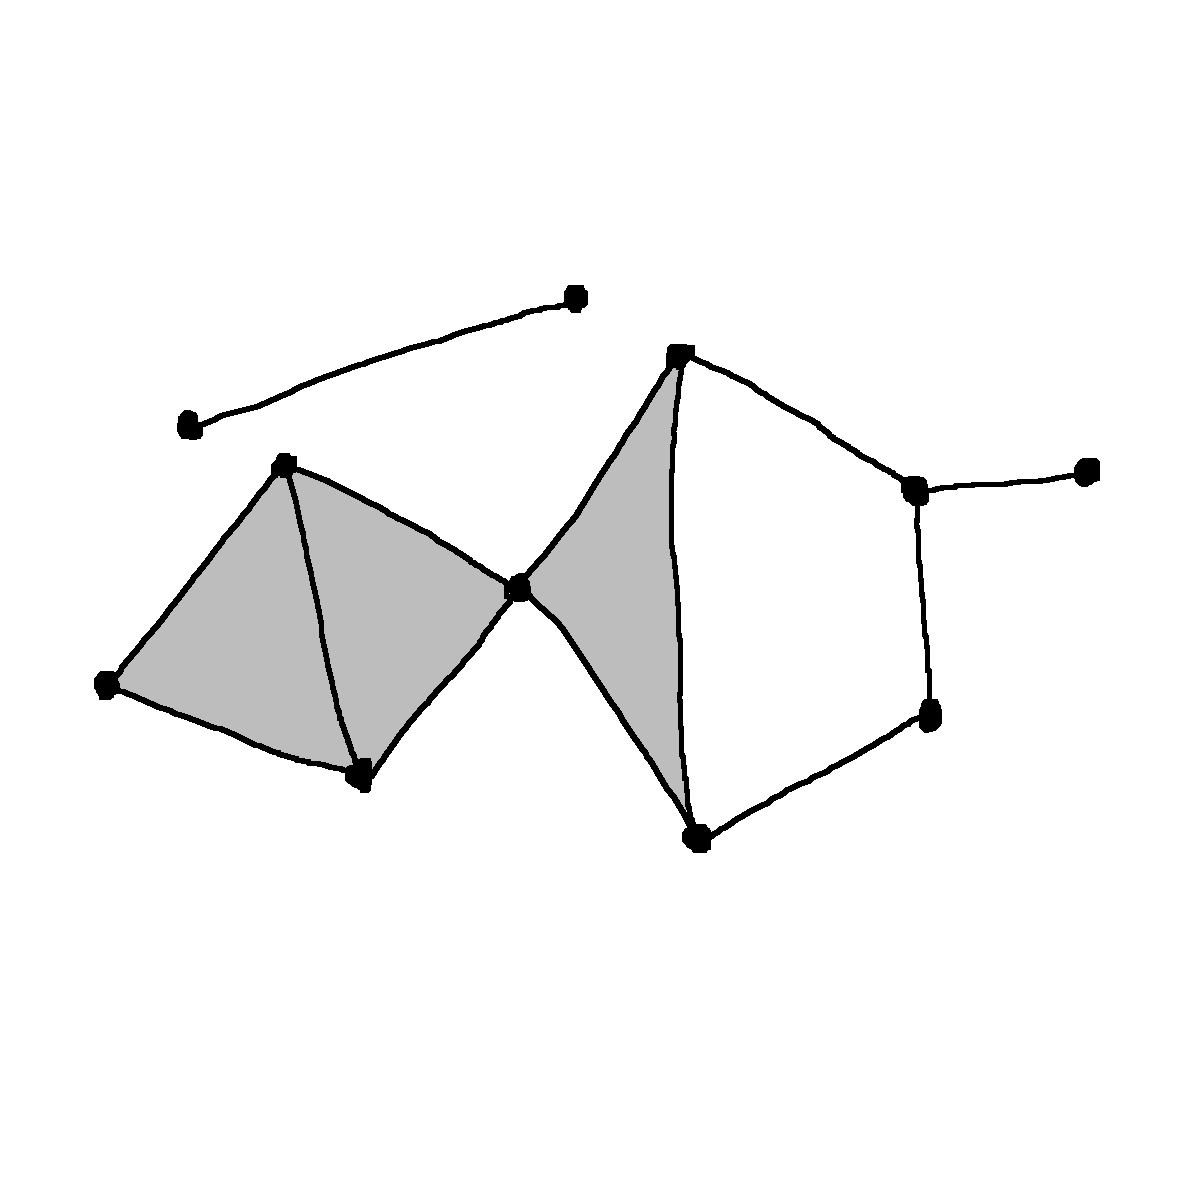
\includegraphics[width=\columnwidth]{\assetspath assets/simplicial-complex-1.png}
        \caption{$\R^2$の単体的複体}
        \label[figure]{fig:simplicial-complex-1}
    \end{minipage}
    \begin{minipage}{0.49\columnwidth}
        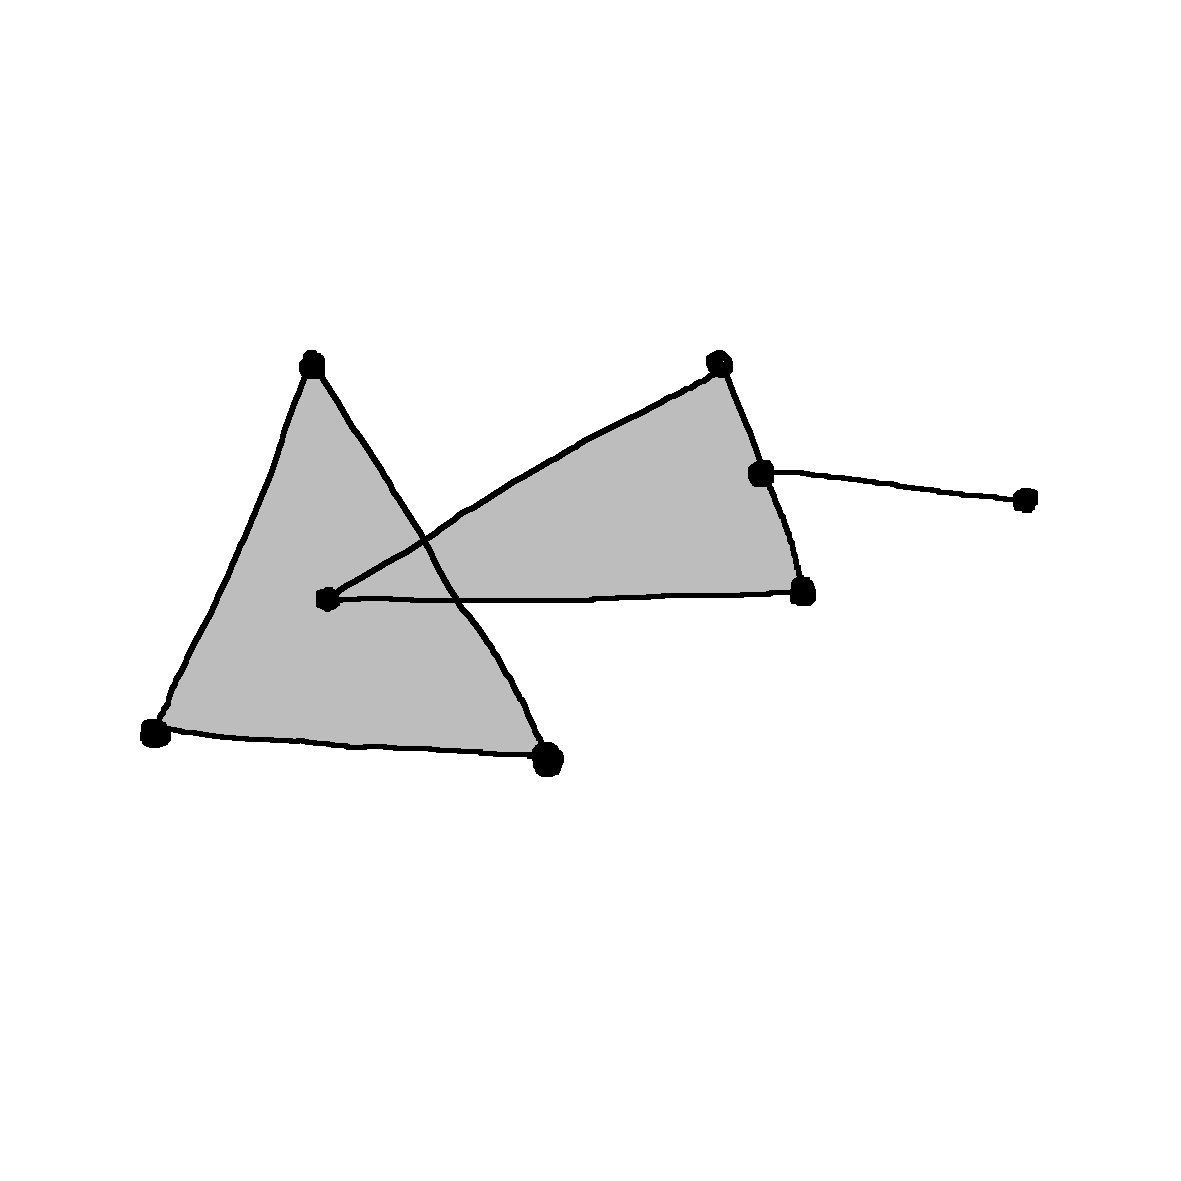
\includegraphics[width=\columnwidth]{\assetspath assets/simplicial-complex-2.png}
        \caption{単体的複体でない例}
        \label[figure]{fig:simplicial-complex-2}
    \end{minipage}
\end{figure}

\begin{definition}[単体分割]
    単体的複体$K$に対し$|K|$が位相空間$X$と同相であるとき、
    $K$を$X$の\term{単体分割}{単体分割}[たんたいぶんかつ]という。
\end{definition}

\begin{definition}[向き付けられた単体的複体]
    $K$を$\R^n$内の単体的複体とする。
    $\Vert(K)$上の半順序であって、各単体$\sigma \in K$上への制限が全順序であるものを
    $K$の\term{向き}[orientation]{向き}[むき]という
    (\cref{fig:oriented-simplicial-complex})。
    以後、単に単体的複体といったときは向きが入っているものとする。
    また、$k$-単体$\sigma$を$\sigma = [v_0 \dots v_k]$と書いたとき、
    $\sigma$には$v_0 < \dots < v_k$なる向きが入っているものとする。
\end{definition}

\begin{figure}
    \centering
    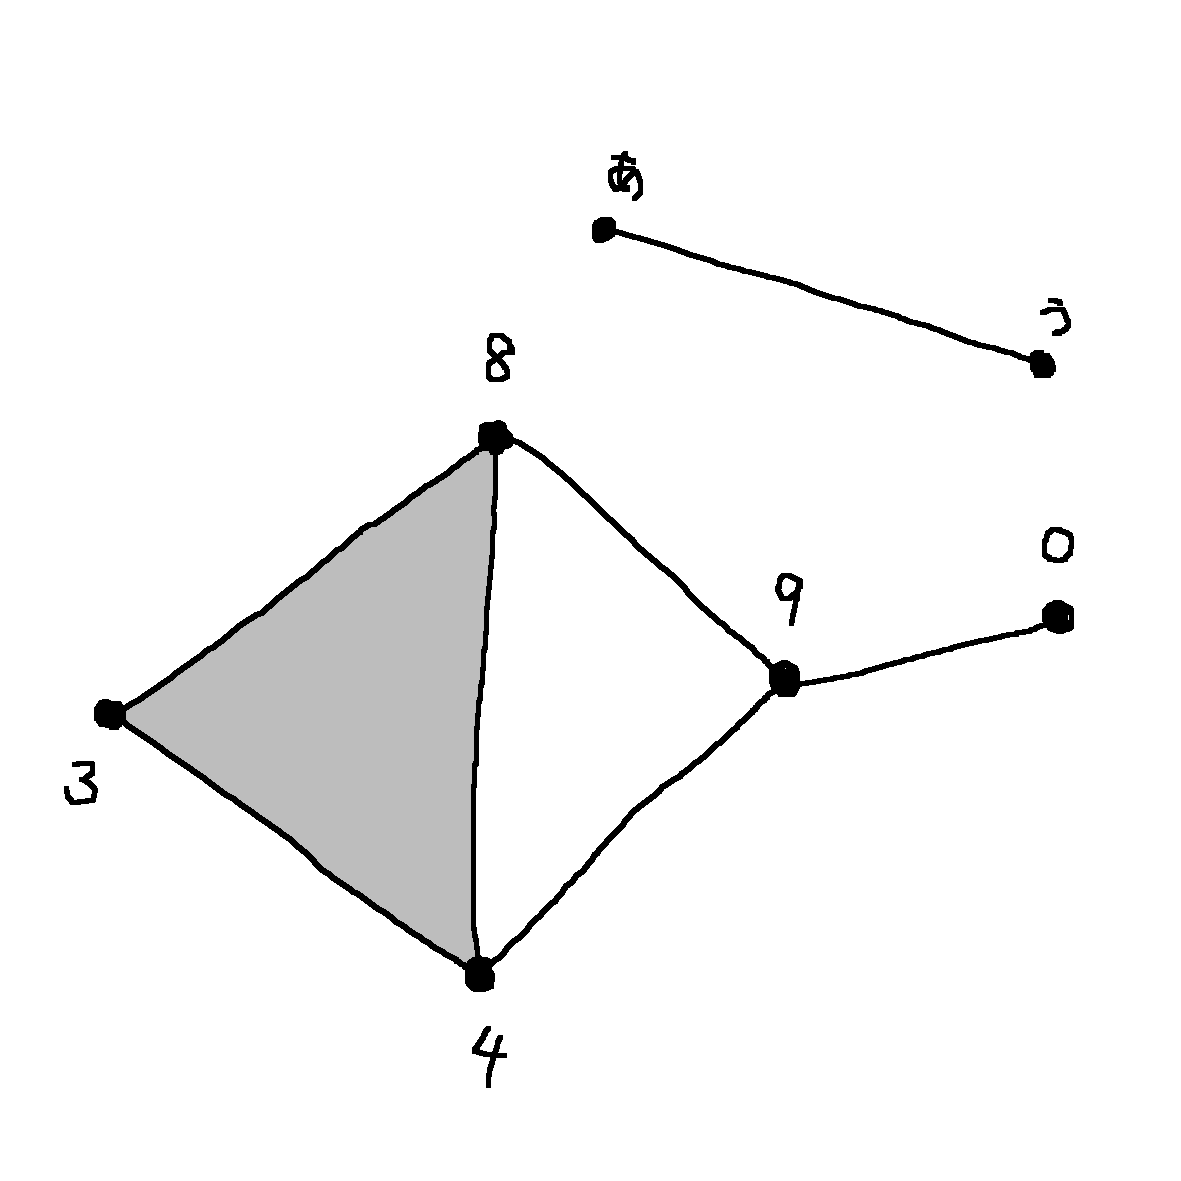
\includegraphics[width=8cm]{\assetspath assets/oriented-simplicial-complex.png}
    \caption{向き付けられた単体的複体}
    \label[figure]{fig:oriented-simplicial-complex}
\end{figure}

\subsection{単体的ホモロジー}

\TODO{単体的ホモロジーはアファインホモロジーと違う?}

\begin{definition}[単体的チェイン群]
    $K$を単体的複体とする。
    各$p \in \Z$に対し、
    \term{第$p$単体的チェイン群}[$p$-th simplicial chain group]{単体的チェイン群}[たんたいてきちぇいんぐん]と呼ばれる
    アーベル群$C_p(K)$を以下のように定める。
    \begin{itemize}
        \item $p < 0$のときは$C_p(K) \coloneqq 0$と定める。
        \item $p \ge 0$のときは、
            $C_p(K)$は$K$に属する$p$-単体のすべてにより生成される自由アーベル群であって、
            関係式
            \begin{enumerate}
                \item $p+1$次の置換$\pi$に対し$[v_0 \dots v_p] = \mathrm{sgn}(\pi) [v_{\pi(0)} \dots v_{\pi(p)}]$
            \end{enumerate}
            をみたすものとして定める(ことができる)\footnotemark。
    \end{itemize}
\end{definition}

\footnotetext{
    $C_p(K)$は
    \begin{itemize}
        \item 生成元: $\Vert(K)$の$p + 1$個の元のタプル$(v_0, \dots, v_p)$であって、
            $\{ v_0, \dots, v_p \}$の凸包が$K$に属する($p$次元とは限らない)単体となるもの全体
        \item 関係式:
            \begin{enumerate}
                \item $v_0, \dots, v_p$に重複があれば$(v_0, \dots, v_p) = 0$
                \item $p+1$次の置換$\pi$に対し$(v_0 \dots v_p) = \mathrm{sgn}(\pi) (v_{\pi(0)} \dots v_{\pi(p)})$
            \end{enumerate}
    \end{itemize}
    により表示される群のアーベル化である。
}

\begin{example}[単体的チェイン群の関係式]
    単体的複体
    \begin{equation}
        K \coloneqq \{ [abc], [cbd], [ab], [bc], [ca], [bd], [dc], [a], [b], [c], [d] \}
    \end{equation}
    を考える($K$には向きが入っていることに注意)。
    このとき第2チェイン群の形は
    \begin{equation}
        C_2(K) = \{ \alpha [abc] + \beta [cbd] \colon \alpha, \beta \in \Z \}
    \end{equation}
    である。
    ただし、たとえば$[abc], [bac] \in C_2(K)$に対し$[abc] = -[bac]$が成り立つ。
    これは単体に逆の向きを入れたものが
    チェイン群上での逆元に対応することを表している。
\end{example}

\begin{definition}[単体的チェイン複体]
    \label[definition]{def:simplicial-chain-complex}
    $K$を単体的複体とする。
    群準同型$\partial_p \colon C_p(K) \to C_{p-1}(K)$を
    次のように定める:
    \begin{itemize}
        \item $p \ge 1$なら、$\partial_p$は
            \begin{equation}
                \label[equation]{eq:simplicial-boundary-homomorphism}
                [v_0 \dots v_p] \mapsto \sum_{i=0}^{p} (-1)^{i} [v_0 \dots \hat{v}_i \dots v_p]
            \end{equation}
            により定まる準同型とし、
        \item $p \le 0$なら、$\partial_p \coloneqq 0$とする。
    \end{itemize}
    このとき、列
    \begin{equation}
        \begin{tikzcd}
            \cdots \ar{r}
            & C_{p+1}(K) \ar{r}{\partial_{p+1}}
            & C_p(K) \ar{r}{\partial_{p}}
            & C_{p-1}(K) \ar{r}
            & \cdots
        \end{tikzcd}
    \end{equation}
    はチェイン複体となる。
    これを$K$の\term{単体的チェイン複体}[simplicial chain complex]{単体的チェイン複体}[たんたいてきちぇいんふくたい]という。
\end{definition}

\begin{proof}[チェイン複体となることの証明]
    $\partial_{p-1} \circ \partial_p = 0$を示せばよい。
    $p \le 1$のときは明らか。
    $p > 1$のときは\cref{eq:simplicial-boundary-homomorphism}に基づいて確かめればよい。
    たとえば$p = 2$の場合を確かめると
    \begin{alignat}{1}
        \partial_1 \circ \partial_2 ([v_0 v_1 v_2])
            &= \partial_1 ([v_1 v_2] - [v_0 v_2] + [v_0 v_1]) \\
            &= \partial_1 ([v_1 v_2]) - \partial_1([v_0 v_2]) + \partial_1([v_0 v_1]) \\
            &= ([v_2] - [v_1]) - ([v_2] - [v_0]) + ([v_1] - [v_0]) \\
            &= 0
    \end{alignat}
    となり、たしかに成り立つ。
    $p > 2$の場合は省略。
\end{proof}

\begin{definition}[単体的ホモロジー群]
    \cref{def:simplicial-chain-complex}の状況で、
    \begin{itemize}
        \item $\Ker(\partial_p)$を$Z_p(K)$と書く。
        \item $\Im(\partial_{p+1})$を$B_p(K)$と書く。
        \item 単体的チェイン複体のホモロジー群$Z_p(K) / B_p(K)$を
            $K$の\term{単体的ホモロジー群}[simplicial homology group]{単体的ホモロジー群}[たんたいてきほもろじーぐん]といい、
            $H_p(K)$と書く。
    \end{itemize}
\end{definition}

\begin{example}[$0$-単体の単体的ホモロジー群]
    \label[example]{ex:0-simplex-homology}
    $0$-単体の定める単体的複体$K = \{ [v_0] \}$を考える。
    \begin{alignat}{1}
        C_0(K) &= \{ n [v_0] \colon n \in \Z \} \cong \Z \\
        Z_0(K) &= C_0(K) \\
        C_0(K) &= 0
    \end{alignat}
    だから
    \begin{equation}
        H_0(K) = Z_0(K) / B_0(K) = C_0(K) / 0 \cong C_0(K) \cong \Z
    \end{equation}
    である。一方、$k \neq 0$ならば$C_k(K) = 0$だから$H_k(K) = 0$である。
    まとめると
    \begin{equation}
        H_k(K) \cong \begin{cases}
            \Z \quad &\text{if $k = 0$} \\
            0 \quad &\text{if $k \neq 0$}
        \end{cases}
    \end{equation}
    である。
\end{example}

\begin{example}[内部を含まない三角形の単体的ホモロジー群]
    \label[example]{ex:triangle-homology}
    三角形$v_0 v_1 v_2$の周の定める単体的複体
    $K = \{ [v_0 v_1], [v_1 v_2], [v_2 v_0], [v_0], [v_1] \}$を考える。
    表記の簡略化のため
    \begin{alignat}{1}
        &P_j \coloneqq [v_j] \quad (j = 1, 2, 3) \\
        &e_0 \coloneqq [v_1 v_2],\; e_1 \coloneqq [v_2 v_0],\; e_2 \coloneqq [v_0 v_1]
    \end{alignat}
    とおく。
    単体的チェイン群は
    \begin{alignat}{1}
        C_0(K) &\coloneqq \{ aP_0 + bP_1 + cP_2 \colon a, b, c \in \Z \} \\
        C_1(K) &\coloneqq \{ se_0 + te_1 + ue_2 \colon s, t, u \in \Z \}
    \end{alignat}
    である。
    境界作用素$\partial_1 \colon C_1(K) \to C_0(K)$は
    \begin{alignat}{1}
        \partial_1(e_0) &= P_2 - P_1 \\
        \partial_1(e_1) &= P_0 - P_2 \\
        \partial_1(e_2) &= P_1 - P_0
    \end{alignat}
    をみたすから、
    $\partial_1$の基底$P_0, P_1, P_2; e_0, e_1, e_2$に関する行列表示は
    \begin{equation}
        \begin{bmatrix}
            0 & 1 & -1 \\
            -1 & 0 & 1 \\
            1 & -1 & 0
        \end{bmatrix}
        \eqqcolon A
    \end{equation}
    となる。$A$は基本変形により
    \begin{equation}
        \begin{bmatrix}
            1 & 0 & 0 \\
            0 & 1 & 0 \\
            0 & 0 & 0
        \end{bmatrix}
    \end{equation}
    となるから、
    \begin{alignat}{1}
        \rk B_0(K) &= \rk\Im(\partial_1) = \rk\Im(A) = 2 \\
        \rk Z_1(K) &= \rk\Ker(\partial_1) = \rk C_1(K) - \rk\Im(\partial_1) = 3 - 2 = 1
    \end{alignat}
    である。
    一方、$\partial_0 = 0, C_2(K) = 0$より
    \begin{alignat}{1}
        \rk Z_0(K) &= \rk C_0(K) = 3 \\
        \rk B_1(K) &= \rk \Im(\partial_2) = \rk \partial_2(C_2(K)) = 0
    \end{alignat}
    である。
    よって
    \begin{alignat}{1}
        \rk H_0(K) &= \rk Z_0(K) - \rk B_0(K) = 3 - 2 = 1 \\
        \rk H_1(K) &= \rk Z_1(K) - \rk B_1(K) = 1 - 0 = 1
    \end{alignat}
    である。
    したがって
    \begin{equation}
        H_k(K) \cong \begin{cases}
            \Z \quad &\text{if $k = 0, 1$} \\
            0 \quad &\text{otherwise}
        \end{cases}
    \end{equation}
    を得る。
    とくに$Z_1(K)$の基底として$e_0 + e_1 + e_2$がとれるが、これは三角形の周である。
    いま$B_1(K) = 0$だから、自然な準同型$Z_1(K) \to H_1(K)$による$e_0 + e_1 + e_2$の像が$H_1(K)$の基底となる。
    よって、大まかには三角形の周が$H_1(K)$の基底となるようなイメージである。
\end{example}

\begin{theorem}[単体的ホモロジー群と特異ホモロジー群]
    $X$を位相空間とする。
    $X$が単体分割$K$をもつとき、
    $H_p(X) \cong H_p(K) \; (p \in \Z)$である。
\end{theorem}

\begin{proof}
    省略
\end{proof}



% ----------------------------------------------------------------------------
%
% ----------------------------------------------------------------------------
\section{Polygonal Presentations}

ここでは球面やトーラスなど
平面のホモロジーを計算するための特別な手法を導入する。

\begin{definition}[2次元単体的複体]
    $X$を2次元のCW複体とする。
    $X$の構成に用いられた$p$-セル全体の集合 ($p = 0, 1, 2$) をそれぞれ$V, E, F$と書き、
    各集合の元をそれぞれ
    \term{頂点}[vertex]{頂点}[ちょうてん]、
    \term{辺}[edge]{辺}[へん]、
    \term{面}[face]{面}[めん]という。
    $X$を$(V, E, F)$と書き、
    \term{2次元単体的複体}{2次元単体的複体}[2じげんたんたいてきふくたい]という。
\end{definition}

用語がややこしいが、2次元単体的複体は\highlight{単体的複体ではない}。

\begin{definition}[頂点・辺・面の記法]
    \TODO{}
\end{definition}

\begin{definition}[2次元単体的複体から定まるチェイン複体]
    $X = (V, E, F)$を2次元単体的複体とする。
    各$p \in \Z$に対し、
    アーベル群$C_p(X)$を以下のように定める。
    \begin{itemize}
        \item $p = 0, 1, 2$のときは、
            $C_p(X)$はそれぞれ$V, E, F$により生成される自由アーベル群と定める。
        \item それ以外のときは$C_p(X) \coloneqq 0$と定める。
    \end{itemize}
    また、群準同型$\partial_p \colon C_p(X) \to C_{p-1}(X)$を
    次のように定める:
    \begin{itemize}
        \item $p = 0, 1, 2$のときは
            \begin{alignat}{1}
                \partial_0([v]) &\coloneqq 0, \\
                \partial_1([uv]) &\coloneqq [v] - [u], \\
                \partial_2((e_0 \dots e_k)) &\coloneqq e_0 + \dots + e_k
            \end{alignat}
        \item それ以外のときは$\partial_p \coloneqq 0$とする。
    \end{itemize}
\end{definition}

\begin{theorem}[2次元単体的ホモロジーの細分による不変性]
    \TODO{}
\end{theorem}

\begin{proof}
    省略
\end{proof}

\begin{example}[2次元トーラス]
    \TODO{}
\end{example}

% ----------------------------------------------------------------------------
%
% ----------------------------------------------------------------------------
\section{Eilenberg-Steenrod 公理系}

\TODO{}

% ----------------------------------------------------------------------------
%
% ----------------------------------------------------------------------------
\newpage
\section{演習問題}

\subsection{問題セット 7}

\begin{problem}[幾何学II 演習問題7.1]
    空間$S^1 \times D^2$において、
    集合$S^1 \times \{ 0 \}$を一点に縮めて得られる空間の
    整係数ホモロジー群を求めよ。
\end{problem}

\begin{proof}[解答.]
    特異ホモロジーの Mayer-Vietoris 完全列を用いる。
    $X \coloneqq (S^1 \times D^2) / (S^1 \times \{ 0 \})$とおき、
    標準射$S^1 \times D^2 \to X$を$\pi$とおく。
    \begin{alignat}{1}
        X_0 &\coloneqq \pi(S^1 \times [0, 1/2)) \\
        X_1 &\coloneqq \pi(S^1 \times (0, 1])
    \end{alignat}
    とおくと$X_0, X_1$は$X$の開集合であって
    $X = X_0 \cup X_1$をみたす。
    包含写像に名前をつけて
    \begin{equation}
        \begin{tikzcd}
            & X_0
                \ar[end anchor=north west]{rd}{j_0} \\
            X_0 \cap X_1
                \ar[start anchor=north east]{ru}{i_0}
                \ar[start anchor=south east]{rd}[swap]{i_1}
                && X_0 \cup X_1 = X \\
            & X_1
                \ar[end anchor=south west]{ru}[swap]{j_1}
        \end{tikzcd}
    \end{equation}
    とおく。
    $X_0 \cap X_1 = \pi(S^1 \times (0, 1/2)) \neq \emptyset$だから
    被約ホモロジーの Mayer-Vietoris 完全列
    \begin{equation}
        \begin{tikzcd}
            \cdots
                \ar{r}
                & \widetilde{H}_{p + 1}(X)
                    \ar{r}
                & \widetilde{H}_p(X_0 \cap X_1)
                    \ar{r}{(i_{0*}, -i_{1*})}
                & \widetilde{H}_p(X_0) \oplus \widetilde{H}_p(X_1)
                    \ar{r}{j_{0*} + j_{1*}}
                & \widetilde{H}_p(X)
                    \ar{r}
                & \cdots
        \end{tikzcd}
    \end{equation}
    を得る。
    ここで$i_1 \colon X_0 \cap X_1 \to X_1$は変形レトラクションだから、
    $X_0 \simeqhe *$であることとあわせて
    $(i_{0*}, -i_{1*})$は同型
    $\widetilde{H}_p(X_0 \cap X_1)
        \cong \widetilde{H}_p(X_0) \oplus \widetilde{H}_p(X_1)$
    を与える。
    よって Mayer-Vietoris 完全列から
    $\widetilde{H}_p(X) = 0$が従う。
    $X$が弧状連結 (\because $X$は弧状連結空間$S^1 \times D^2$の連続写像による像) ゆえに 
    $H_0(X) \cong \Z$であることとあわせて
    \begin{equation}
        H_p(X) \cong \begin{cases}
            \widetilde{H}_p(X) = 0 & (p \geq 1) \\
            \Z & (p = 0)
        \end{cases}
    \end{equation}
    を得る。
\end{proof}

\begin{problem}[幾何学II 演習問題7.2]
    空間$S^1 \times D^2$において、
    集合$S^1 \times S^1$を一点に縮めて得られる空間の
    整係数ホモロジー群を求めよ。
\end{problem}

\begin{proof}[解答 1.]
    Mayer-Vietoris を用いる。
    \TODO{}
\end{proof}

\begin{proof}[解答 2.]
    胞体分割を用いる。
    $X \coloneqq (S^1 \times D^2) / (S^1 \times S^1)$とおき、
    標準射$S^1 \times D^2 \to X$を$\pi$とおく。
    $X$の胞体分割を
    \begin{alignat}{1}
        X &= e^0 \sqcup e^2 \sqcup e^3 \\
        e^0 &\coloneqq \pi(S^1 \times S^1) \\
        e^2 &\coloneqq \pi(\{ 1 \} \times \mathring{D}^2) \\
        e^3 &\coloneqq \pi((S^1 \setminus \{ 1 \}) \times \mathring{D}^2)
    \end{alignat}
    で与えることができる。
    したがってチェイン複体
    \begin{equation}
        \begin{tikzcd}
            0
                \ar{r}
                & \underbrace{C_3(X)}_{
                    \cong \Z
                }
                    \ar{r}{\del_3}
                & \underbrace{C_2(X)}_{
                    \cong \Z
                }
                    \ar{r}{\del_2}
                & \underbrace{C_1(X)}_{
                    = 0
                }
                    \ar{r}{\del_1}
                & \underbrace{C_0(X)}_{
                    \cong \Z
                }
                    \ar{r}
                & 0
        \end{tikzcd}
    \end{equation}
    を得る。
    $C_1(X) = 0$より$\del_1 = 0, \del_2 = 0$である。

    $\del_3$を求める。
    空間対の射
    $(X^2, X^1) \twoheadrightarrow (X^2 / X^1, *) \to (S^2, *)$
    を$\pi^2$とおき
    $[e^3 : e^2] = \deg (\pi^2 \circ \varphi^3|_{S^2})$
    を求める。
    ここで特性写像$\varphi^3$は、
    $S^2 \subset D^3$を次のように写すものとしてよい。
    すなわち
    $\{ (x, y, z) \in S^2 \mid z \ge 1 / 2 \}, \;
        \{ (x, y, z) \in S^2 \mid z \le - 1 / 2 \}$は
    これらを平面$z = 0$に射影した像を$D^2$とみて
    $\wb{e^2}$に写し、
    $\{ (x, y, z) \in S^2 \mid - 1 / 2 \le z \le 1 / 2 \}$は
    $e^0$に写す。
    すると$S^2$の平面$x = 0$に関する鏡映$r$により
    \begin{equation}
        \pi^2 \circ \varphi^3|_{S^2} \circ r
            = \pi^2 \circ \varphi^3|_{S^2}
    \end{equation}
    が成り立つ。したがって
    $[e^3 : e^2] = \deg (\pi^2 \circ \varphi^3|_{S^2}) = 0$である。
    よって$\del_3 = 0$である。

    以上より$H_p(X) = C_p(X)$を得る。
    したがって
    \begin{equation}
        H_p(X) \cong \begin{cases}
            \Z & (p = 0, 2, 3) \\
            0 & (p = 1) \\
            0 & (\text{otherwise})
        \end{cases}
    \end{equation}
    である。
\end{proof}

\begin{problem}[幾何学II 演習問題7.3]
    Klein の壺$K$の胞体分割を与え、
    それを用いて整係数ホモロジー群を求めよ。
\end{problem}

\begin{answer}
    $K$は
    $(0, y) \sim (1, 1 - y), \; (x, 0) \sim (x, 1)$
    により生成される$I \times I$上の同値関係$\sim$
    による商空間と考え、
    商写像$I \times I \to K$を$\pi$とおく。
    以下$X \coloneqq K$と書く。
    $X$の胞体分割を
    \begin{alignat}{1}
        X &= e^0 \cup e^1_1 \cup e^1_2 \cup e^2 \\
        e^0 &\coloneqq \{ \pi(0, 0) \} \\
        e^1_1 &\coloneqq \pi(\mathring{I} \times \{ 0 \}) \\
        e^1_2 &\coloneqq \pi(\{ 0 \} \times \mathring{I}) \\
        e^2 &\coloneqq \pi(\mathring{I} \times \mathring{I})
    \end{alignat}
    で与えることができる。
    セル$e^k_i$の特性写像を$\varphi^k_i \colon D^k \to X^k \subset X$とおく。
    上の胞体分割より、チェイン複体
    \begin{equation}
        \begin{tikzcd}
            0
                \ar{r}
                & \underbrace{C_2(X)}_{
                    \cong \Z
                }
                    \ar{r}{\del_2}
                & \underbrace{C_1(X)}_{
                    \cong \Z \oplus \Z
                }
                    \ar{r}{\del_1}
                & \underbrace{C_0(X)}_{
                    \cong \Z
                }
                    \ar{r}
                & 0
        \end{tikzcd}
    \end{equation}
    を得る。

    ホモロジーを求めるために境界写像を計算する。
    $\del_1$を考える。
    \begin{alignat}{1}
        \del_1 e^1_1 &= e^0 - e^0 = 0 \\
        \del_1 e^1_2 &= e^0 - e^0 = 0
    \end{alignat}
    だから$\del_1 = 0$である。

    $\del_2$を考える。
    空間対の射
    $(X^1, X^0) \twoheadrightarrow (X^1 / (X^0 \cup e^1_2), *) \to (S^1, *)$
    を$\pi^1_1$とおき
    $[e^2 : e^1_1] = \deg (\pi^1_1 \circ \varphi^2|_{S^1})$を求める。
    ここで特性写像$\varphi^2$は
    $S^1 \subset D^2$上の点を次のように写すものとしてよい。
    すなわち、
    $\varphi^2$は$S^1$上の点を
    $\del (I \times I)$上の点に反時計回りに
    等間隔に写し、さらに$\pi$で写すものとする。
    すると$S^1$の適当な鏡映$r$に対し
    \begin{equation}
        \pi^1_1 \circ \varphi^2|_{S^1} \circ r
            = \pi^1_1 \circ \varphi^2|_{S^1}
    \end{equation}
    が成り立つ。
    よって$[e^2 : e^1_1] = \deg (\pi^1_1 \circ \varphi^2|_{S^1}) = 0$である。

    つぎに空間対の射
    $(X^1, X^0) \twoheadrightarrow (X^1 / (X^0 \cup e^1_1), *) \to (S^1, *)$
    を$\pi^1_2$とおき
    $[e^2 : e^1_2] = \deg (\pi^1_2 \circ \varphi^2|_{S^1})$を求める。
    \TODO{写像度の局所化が必要}
\end{answer}

\begin{problem}[幾何学II 演習問題7.4]
    3次元トーラス$T^3 = S^1 \times S^1 \times S^1$の胞体分割を与え、
    それを用いて整係数ホモロジー群を求めよ。
\end{problem}

\begin{answer}
    \TODO{}
\end{answer}

\begin{problem}[幾何学II 演習問題7.5]
    次の集合$X_1, X_2$の和集合$X = X_1 \cup X_2$の
    整係数ホモロジー群を求めよ。
    \begin{alignat}{1}
        X_1 &\coloneqq \{
            (x, y, z) \in \R^3 \mid
            (x + 1)^2 + y^2 + z^2 = 4 \sqrt{(x + 1)^2 + y^2} - 3
        \} \\
        X_2 &\coloneqq \{
            (x, y, z) \in \R^3 \mid
            (x - 1)^2 + y^2 + z^2 = 4 \sqrt{(x - 1)^2 + y^2} - 3
        \}
    \end{alignat}
\end{problem}

\begin{answer}
    \TODO{}
\end{answer}

\begin{problem}[幾何学II 演習問題7.6]
    階数1の$2 \times n$行列全体のなす集合$X$の
    整係数ホモロジー群を求めよ
\end{problem}

\begin{answer}
    \TODO{}
\end{answer}



\end{document}